% A LaTeX template for ARTICLE version of the MSc Thesis submissions to 
% Politecnico di Milano (PoliMi) - School of Industrial and Information Engineering
%
% S. Bonetti, A. Gruttadauria, G. Mescolini, A. Zingaro
% e-mail: template-tesi-ingind@polimi.it
%
% Last Revision: October 2021
%
% Copyright 2021 Politecnico di Milano, Italy. Inc. NC-BY

\documentclass[11pt,a4paper]{article} 

%------------------------------------------------------------------------------
%	REQUIRED PACKAGES AND  CONFIGURATIONS
%------------------------------------------------------------------------------
% PACKAGES FOR TITLES
\usepackage{titlesec}
\usepackage{color}

% PACKAGES FOR LANGUAGE AND FONT
\usepackage[utf8]{inputenc}
\usepackage[english]{babel}
\usepackage[T1]{fontenc} % Font encoding
\usepackage{dsfont} % For \mathds (e.g., \R)

% PACKAGES FOR IMAGES
\usepackage{graphicx}
\graphicspath{{Images/}}
\usepackage{eso-pic} % For the background picture on the title page
\usepackage{subfig} % Numbered and caption subfigures using \subfloat
\usepackage{caption} % Coloured captions
\usepackage{transparent}

% STANDARD MATH PACKAGES
\usepackage{amsmath}
\usepackage{amsthm}
\usepackage{bm}
\usepackage{amssymb}
\usepackage[overload]{empheq}  % For braced-style systems of equations

% PACKAGES FOR TABLES
\usepackage{tabularx}
\usepackage{longtable} % tables that can span several pages
\usepackage{colortbl}

% PACKAGES FOR ALGORITHMS (PSEUDO-CODE)
\usepackage{algorithm}
\usepackage{algorithmic}

% PACKAGES FOR REFERENCES & BIBLIOGRAPHY
\usepackage[colorlinks=true,linkcolor=black,anchorcolor=black,citecolor=black,filecolor=black,menucolor=black,runcolor=black,urlcolor=black]{hyperref} % Adds clickable links at references
\usepackage{cleveref}
\usepackage[square, numbers, sort&compress]{natbib} % Square brackets, citing references with numbers, citations sorted by appearance in the text and compressed
\bibliographystyle{plain} % You may use a different style adapted to your field

% PACKAGES FOR THE APPENDIX
\usepackage{appendix}

% PACKAGES FOR ITEMIZE & ENUMERATES 
\usepackage{enumitem}

% OTHER PACKAGES
\usepackage{amsthm,thmtools,xcolor} % Coloured "Theorem"
\usepackage{comment} % Comment part of code
\usepackage{fancyhdr} % Fancy headers and footers
\usepackage{lipsum} % Insert dummy text
\usepackage{tcolorbox} % Create coloured boxes (e.g. the one for the key-words)

%	ADD YOUR PACKAGES (be careful of package interaction)
\usepackage{nicefrac}
\usepackage{cancel}
\usepackage{color}
\usepackage{chngcntr} %USATO PER RESETTARE CONTATORE EQUAZIONI AD OGNI TEOREMA
\usepackage{cancel} %USATO PER SEMPLIFICARE LE EQUAZIONI
\usepackage{hyperref} %USATO PER COLLEGAMENTI IPERTESTUALI NEL DOCUMENTO
\usepackage{nicematrix} %USATO PER TABELLE NUMERABILITA' Q
\usepackage{mathrsfs} %USATO PER NUOVI FONT
\usepackage{nccmath} %USATO PER \cfrac
\usepackage{tcolorbox} % PER I BOX COLORATI
\usepackage{multicol} % Per mettere multipli grafici in riga, come alternativa all'utilizzo dei minipage. 
\usepackage{changepage} % usato per allineare un intero paragrafo a 0.25cm dal margine sinistro
\usepackage{tikz}
\usepackage{tikz-3dplot}
\usetikzlibrary{arrows.meta} % For better arrows
\usepackage{physics} % FOR RESTRICTION OPERATOR
\usepackage{listings}
\usepackage{booktabs}
\usepackage{ upgreek }
\usepackage{pgffor}
\usepackage{placeins}

%-------------------------------------------------------------------------
%	NEW COMMANDS DEFINED
%-------------------------------------------------------------------------
% EXAMPLES OF NEW COMMANDS -> here you see how to define new commands
\newcommand{\bea}{\begin{eqnarray}} % Shortcut for equation arrays
\newcommand{\eea}{\end{eqnarray}}
\newcommand{\e}[1]{\times 10^{#1}}  % Powers of 10 notation
\newcommand{\mathbbm}[1]{\text{\usefont{U}{bbm}{m}{n}#1}} % From mathbbm.sty
\newcommand{\pdev}[2]{\frac{\partial#1}{\partial#2}}

\newcommand{\C}{\mathds{C}}
\newcommand{\R}{\mathds{R}}
\newcommand{\Q}{\mathds{Q}}
\newcommand{\Z}{\mathds{Z}}
\newcommand{\N}{\mathds{N}}
\newcommand{\Interv}{\text{I}}
\newcommand{\inducP}{\text{P}} % Simbolo per la P di proposizione induttiva ('induc' <-> 'inductive')
\renewcommand{\abs}[1]{\left| #1 \right| } % Definizione comoda ed operativa per il valore assoluto
\renewcommand{\vec}[1]{\underline{#1}} %underlined vector instead of arrow over vector

\let\oldforall\forall
\renewcommand{\forall}{\oldforall \; }
\let\oldexists\exists
\renewcommand{\exists}{\oldexists \; }
\let\oldnexists\nexists
\renewcommand{\nexists}{\oldnexists \; }
\let\oldsetminus\setminus
\renewcommand{\setminus}{\raisebox{1pt}{$\;\oldsetminus\, $}}
\let\oldcancel\cancel
\renewcommand\cancel[2][red]{\renewcommand\CancelColor{\color{#1}}\oldcancel{#2}}
\newcommand{\existsoneonly}{\oldexists ! \;}
\newcommand{\commadotscomma}{, \; ... \enspace ,\,}
\newcommand{\sumdotssum}{+ \enspace ... \enspace +}
\newcommand{\proddotsprod}{\cdot \enspace ... \enspace \cdot}
\newcommand{\leqdotsleq}{\leq \; ... \; \leq}
\newcommand{\geqdotsgeq}{\geq \; ... \; \geq}
\newcommand{\eqdotseq}{= \; ... \; =}
\newcommand{\ldotsl}{< \; ... \; <}
\newcommand{\mdotsm}{> \; ... \; >}
\newcommand{\neqdotsneq}{\neq \; ... \; \neq}
\newcommand{\Reynolds}{\mathbbm{R}e} % Reynold's number declaration
\DeclareMathOperator{\sign}{sgn}
\DeclareMathOperator{\Real}{Re}
\DeclareMathOperator{\Img}{Im}
\DeclareMathOperator{\Div}{div}
\DeclareMathOperator{\Riv}{rot}

\newcommand\tab[1][0.25cm]{\hspace*{#1}}
\newcommand{\arraystretchvalue}{1.3}
\newcommand{\sepHpThConEq}{17}
\newcommand{\mystrut}{\rule{0pt}{\ht\strutbox}} % Serve per la grafica di alcuni esponenti frazionari, in modo che il punto da cui partano sia più in alto del classico testo. 
\tdplotsetmaincoords{80}{40} %POV of camera for 3D plots
\graphicspath{{Images/Test_cases/3D/Test_1/}{Images/Test_cases/3D/Test_1/Screenshots/}{Images}{Images/Test_cases/3D/Test_2/}{Images/Test_cases/3D/Test_2/Screenshots/}{Images/Test_cases/3D/Test_3/}{Images/Test_cases/3D/Test_3/test3cyl/}{Images/Test_cases/3D/Test_3/test3rect/}}
\AfterPreamble{\hypersetup{ %metadata for pdf generation
  pdfauthor={Luca Salmoiraghi, Tobia Grimaldi, Dong Hua Zhu},
  pdftitle={Solving Navier-Stokes equations for the "flow past a cylinder" problem},
  pdfsubject={PDE, CFD}
}}


% Do not change Configuration_files/config.tex file unless you really know what you are doing. 
% This file ends the configuration procedures (e.g. customizing commands, definition of new commands)
\input{Configuration_files/config}

% Insert here the info that will be displayed into your Title page 
% -> title of your work
\renewcommand{\title}{Solving Navier-Stokes equations for the "flow past a cylinder" problem}
% -> author name and surname
\renewcommand{\author}{Tobia Grimaldi}
% -> author ID
\newcommand{\ID}{11127377}
% -> author name and surname
\newcommand{\secondauthor}{Luca Salmoiraghi}
% -> author ID
\newcommand{\secondID}{10849129}
% -> author name and surname
\newcommand{\thirdauthor}{Dong Hua Zhu}
% -> author ID
\newcommand{\thirdID}{10827613}
% -> advisor name and surname
\newcommand{\advisor}{Prof.Alfio Maria Quarteroni}
% IF AND ONLY IF you need to modify the co-supervisors you also have to modify the file Configuration_files/title_page.tex (ONLY where it is marked)
\newcommand{\firstcoadvisor}{Michele Bucelli} % insert if any otherwise comment
% -> academic year
\newcommand{\YEAR}{2025-2026}
% -> abstract (only in English)
\renewcommand{\abstract}{ This research introduces a finite element solver for the incompressible Navier-Stokes equations. Developed using C++ deal.II library, the solver employs stable $\mathbb{P}^{2}/\mathbb{P}^{1}$ elements for space discretisation and the $\theta$-method for time discretisation. The investigation focuses on capturing steady and unsteady laminar flow patterns in the classical CFD benchmark "flow past a cylinder", evaluating performance of the solver through drag and lift coefficients analysis.}

% -> key-words (only in English)
\newcommand{\keywords}{Navier-Stokes equations, Finite Element Method (FEM), Flow past a cylinder, deal.II library, CFD benchmark}

%-------------------------------------------------------------------------
%	BEGIN OF YOUR DOCUMENT
%-------------------------------------------------------------------------
\begin{document}

%-----------------------------------------------------------------------------
% TITLE PAGE
%-----------------------------------------------------------------------------
% Do not change Configuration_files/TitlePage.tex (Modify it IF AND ONLY IF you need to add or delete the Co-advisors)
% This file creates the Title Page of the document
% DO NOT REMOVE SPACES BETWEEN LINES!

\AddToShipoutPicture*{\BackgroundPic}

\hspace{-0.6cm}
\includegraphics[width=0.6\textwidth]{logo_polimi_ing_indinf.eps}

\vspace{-1mm}
\Large{\textbf{\color{bluePoli}{\title}}}\\

\vspace{-0.2cm}

\vspace{-0.2cm}
\large{\textbf{\author, \ID}} \\
\large{\textbf{\secondauthor, \secondID}} \\
\large{\textbf{\thirdauthor, \thirdID}}
\small \normalfont

\vspace{11pt}

\centerline{\rule{1.0\textwidth}{0.4pt}}

\begin{center}
\begin{minipage}[t]{.24\textwidth}
\begin{minipage}{.90\textwidth}
\noindent
\scriptsize{\textbf{Advisor:}} \\
\advisor \\
\\
\textbf{Co-advisors:} \\ % leave it if any co-advisor otherwise comment
\firstcoadvisor \\ % leave it if any co-advisor otherwise comment
% \secondcoadvisor \\ % leave it if you have more that one co-advisor otherwise comment (if you have more than two co-advisors just copy&paste this line writing \thirdcoadvisor, \fourthcoadvisor, ecc. (REMEMBER to modify also the main.txt)
\\ % leave it if any co-advisor otherwise comment
\textbf{Academic year:} \\
\YEAR \\
\\
\end{minipage}
\end{minipage}% This must go next to `\end{minipage}`
\begin{minipage}{.74\textwidth}
\noindent \textbf{\color{bluePoli} Abstract:} {\abstract}
\end{minipage}
\end{center}

\vspace{15pt}

\begin{tcolorbox}[arc=0pt, boxrule=0pt, colback=bluePoli!60, width=\textwidth, colupper=white]
    \textbf{Key-words:} \keywords
\end{tcolorbox}

\vspace{12pt}

%%%%%%%%%%%%%%%%%%%%%%%%%%%%%%
%%     THESIS MAIN TEXT     %%
%%%%%%%%%%%%%%%%%%%%%%%%%%%%%%

%-----------------------------------------------------------------------------
% INTRODUCTION
%-----------------------------------------------------------------------------
\section{Introduction}
\label{sec:introduction}
This document presents an overview of the most prominent finite element methods for solving the incompressible Navier-Stokes equations to simulate the 2D/3D benchmark problem "flow past a cylinder" for different values of the Reynolds number $\Reynolds \leq 200$. \\
This first section is intended to be a brief introduction to the physical and mathematical problem of interest, in particular with respect to the equations that model the physical situation and weak formulation of such equations. \\
%TODO: Specify in some way that this first part is inspired to Quarteroni's own book?
\subsection{Introduction to Navier-Stokes equations}
\label{subsec:introduction_navier_stokes}
The celebrated Navier-Stokes equations describe the motion of a fluid, whose density $\rho$ is constant, in a domain $\Omega \subset \R^{d}$ (with $d = 2, \, 3$). In the most general version, they read as follows \cite{Quarteroni2017}: 
\begin{equation}
    \label{eq:navier_stockes_general}
    \left\{
    \begin{aligned}
    &\frac{\partial \vec{u}}{\partial t} - \Div\left[ \nu \left( \nabla \vec{u} + \nabla \vec{u}^{T}\right) \right] + (\vec{u} \cdot \nabla)\vec{u} + \nabla p = \vec{f} \quad & \vec{x} \in \Omega, \, t > 0 \\
    &\Div(\vec{u}) = 0 & \vec{x} \in \Omega, \, t > 0
    \end{aligned}
    \right.
\end{equation}
with $\vec{u} = \vec{u}(\vec{x}, \, t)$ being the velocity of the fluid, $\nu$ the kinematic viscosity, $p$ the pressure divided by the density (which will be addressed simply as "pressure" from now on) and $\vec{f}$ a forcing term per unit of mass, which is supposed to be an element of $L^{2}\left(\R^{+}; \, \left[L^{2}(\Omega) \right]^{d}\right)$ (to say, for each time $t \in \R^{+}$, each component of $\vec{f}$ is in $L^{2}(\Omega)$).
Each of the two equations has a precise meaning: the second represents conservation of mass (the so called "continuity equation"), whilst the first is the conservation of linear momentum, where the term $- \Div\left[ \nu \left( \nabla \vec{u} + \nabla \vec{u}^{T}\right) \right]$ describes molecular diffusion, while $(\vec{u} \cdot \nabla)\vec{u}$ convective transport. \\
When $\nu$ is constant, from the continuity equation it is possible to obtain the following:
\begin{equation*}
    \Div\left[ \nu \left( \nabla \vec{u} + \nabla \vec{u}^{T}\right) \right] = \nu \left(\Delta \vec{u} + \nabla \Div(\vec{u}) \right) = \nu \Delta \vec{u}
\end{equation*}
%TODO: Find suitable reference for the continuity equation
Therefore, the set of equations \eqref{eq:navier_stockes_general} can be rewritten in the equivalent form: 
\begin{equation}
    \label{eq:navier_stockes_incompressible}
    \left\{
    \begin{aligned}
    &\frac{\partial \vec{u}}{\partial t} - \nu \Delta \vec{u} + (\vec{u} \cdot \nabla)\vec{u} + \nabla p = \vec{f} \quad & \vec{x} \in \Omega, \, t > 0 \\
    &\Div(\vec{u}) = 0 & \vec{x} \in \Omega, \, t > 0
    \end{aligned}
    \right.
\end{equation}
Such equations \eqref{eq:navier_stockes_incompressible} are known as \textbf{incompressible Navier-Stokes equations}, which are the ones that will be considered from now on. \\
Of course, in order for the equations \eqref{eq:navier_stockes_incompressible} to be well posed, both initial and boundary conditions must be provided. Consider therefore $\Gamma_{D}; \, \Gamma_{N} \subseteq \partial\Omega$ such that $\Gamma_{D} \cap \Gamma_{N} = \varnothing$ and $\Gamma_{D} \cup \Gamma_{N} = \partial \Omega$. The required conditions can be expressed as follows: 
\begin{equation}
    \label{eq:boundary_conditions}
    \left\{
    \begin{aligned}
    &\vec{u}(\vec{x}, \, t = 0) = \vec{u}_{0}(\vec{x}) &&\vec{x} \in \Omega \\
    &\vec{u}(\vec{x}, +\, t) = \vec{g}(\vec{x}, t) &&\vec{x} \in \Gamma_{D} \\
    &\left( \nu \frac{\partial \vec{u}}{\partial \hat{\eta}} -p\hat{\eta} \right)(\vec{x}, \, t) = \vec{h}(\vec{x}, \, t) \quad &&\vec{x} \in \Gamma_{N}
    \end{aligned}
    \right.
\end{equation}
where $\hat{\eta}$ is the normal outward unitary vector to $\partial \Omega$.\\
Therefore, this paper will discuss how to numerically solve the equations \eqref{eq:navier_stockes_incompressible} with initial and boundary conditions \eqref{eq:boundary_conditions}. \\
Moreover, if the term
\begin{equation*}
    (\vec{u} \cdot \nabla) \vec{u} = 0
\end{equation*}
the Navier-Stokes equations yield to a linear formulation which is called unsteady Stokes equations (see \ref{subsubsec:stokes_equations}). In general, to study whether such a term is negligible or not, the so called \textbf{Reynolds number} $\Reynolds$ is introduced: 
\begin{equation}
    \label{eq:reynolds_number}
    \Reynolds := \frac{\abs{\vec{U}}L}{\nu}
\end{equation}
where $L$ is the length of the computational domain, $\nu$ is once again the viscosity of the fluid and $\abs{\vec{U}}$ is the modulus of the so-called characteristic speed of the fluid. If $\Reynolds$ is sufficiently small (in general, if $\Reynolds = O(1)$, but this is very application-dependent), Stokes equations approximate well the behaviour of such a fluid.


\subsection{Weak formulation of the Navier-Stokes equations}
The weak formulation for \eqref{eq:navier_stockes_incompressible} with initial and boundary conditions \eqref{eq:boundary_conditions} (where, for simplicity, $\vec{g} = \vec{0} \quad \forall \vec{x} \in \Gamma_{D}$ will be considered) can be obtained as follows: 
\begin{itemize}
    \item Consider a generic test function $\vec{\varphi}$ belonging to a functional space $\mathcal{V}$ (specified further on). Multiply the first of the two equations of \eqref{eq:navier_stockes_incompressible} by $\vec{\varphi}$ and integrate over $\Omega$: 
    \begin{equation}
        \label{eq:weak_form_1.1}
        \int_{\Omega} \frac{\partial \vec{u}}{\partial t} \cdot \vec{\varphi} \, d\Omega \;-\;\int_{\Omega} \nu \Delta \vec{u} \cdot \vec{\varphi} \, d\Omega \;+\; \int_{\Omega} \bigl[ (\vec{u}\cdot\nabla)\vec{u} \bigr] \cdot \vec{\varphi} \, d\Omega \;+\; \int_{\Omega} \nabla p \cdot \vec{\varphi} \, d\Omega \;=\; \int_{\Omega} \vec{f}\cdot \vec{\varphi} \, d\Omega
    \end{equation}
    As a result of the Green's formulae, the followings relations hold:
    \begin{itemize}
        \item $\displaystyle - \int_{\Omega} \nu \Delta \vec{u} \cdot \vec{\varphi} \, d\Omega \; = \; \int_{\Omega} \nu \nabla \vec{u} \cdot \nabla \vec{\varphi} \, d\Omega \; - \; \int_{\partial \Omega} \nu \frac{\partial \vec{u}}{\partial \hat{\eta}} \cdot \vec{\varphi} \, d\gamma,$
        \item $\displaystyle \int_{\Omega} \nabla p \cdot \vec{\varphi} \, d\Omega \; = \; - \int_{\Omega} p \Div(\vec{\varphi}) \, d\Omega \; + \; \int_{\partial \Omega} p \, \vec{\varphi} \cdot \hat{\eta} \, d\gamma.$
    \end{itemize}
    %TODO: Reference to some book where to find Green Formulae
    and by applying such relations in \eqref{eq:weak_form_1.1}, it is possible to obtain:
    \begin{equation}
    \begin{aligned}
        \int_{\Omega} \frac{\partial \vec{u}}{\partial t} \cdot \vec{\varphi} \,  d\Omega \; + \; \nu \int_{\Omega} \nabla \vec{u} \cdot \nabla \vec{\varphi}  \, d\Omega \; + \; \int_{\Omega} [ (\vec{u} \cdot \nabla) \vec{u}] \cdot \vec{\varphi} \, d\Omega \; - \; \int_{\Omega} p \, \Div \left( \vec{\varphi} \right) \, d\Omega \; = \\
        = \; \int_{\Omega} \vec{f} \cdot \vec{\varphi} \, d\Omega \; + \; \int_{\partial \Omega} \left( \nu \frac{\partial \vec{u}}{\partial \hat{\eta}} - p \hat{\eta} \right) \cdot \vec{\varphi}  \, d\gamma \qquad \forall \vec{\varphi} \in \mathcal{V}
        \end{aligned}
    \end{equation}

    \item In a similar way, consider a test function $\psi$ belonging to a functional space $\mathcal{Q}$ (yet to be defined), multiply the second equation of \eqref{eq:navier_stockes_incompressible} and integrate over $\Omega$, in order to obtain: 
    \begin{equation}
        \int_{\Omega} \psi \, \Div(\vec{u}) \, d \Omega \; = \; 0 \qquad \forall \psi \in \mathcal{Q}
    \end{equation}
\end{itemize}
There remains to discuss the choice of the two functional spaces $\mathcal{V}$ and $\mathcal{Q}$: 
\begin{itemize}
    \item $\mathcal{V}$ is chosen in such a way that the test function vanishes on $\Gamma_{D}$, to say: 
    \begin{equation*}
        \mathcal{V} = \left[ H^{1}_{\Gamma_{D}(\Omega)}\right]^{d} = \left\{ \vec{\varphi} \in \left[ H^{1}(\Omega)\right]^{d} \enspace | \enspace \eval{\vec{\varphi}}_{\Gamma_{D}} = 0 \right\}
    \end{equation*}
    where $H^{1}(\Omega) \equiv W^{1; \, 2}(\Omega)$, where $W^{1; \, 2}(\Omega)$ represents the Sobolev 1, 2 space.

    \item The choice of $\mathcal{Q}$ is more delicate. Since $p$ is never derived in \eqref{eq:navier_stockes_incompressible} and as a consequence neither is $\psi$, there is no need to consider Sobolev spaces for defining $\mathcal{Q}$. If $\Gamma_{N} \neq \varnothing$ then it is sufficient to consider $\mathcal{Q} = L^{2}(\Omega)$. On the other hand, if $\Gamma_{N} = \varnothing$, then the pressure appears in $\eqref{eq:navier_stockes_incompressible}$ exclusively in terms of its gradient, hence if $\tilde{p}$ is a solution of the equations, then $(\tilde{p} + c)$ with $c \in \R$ would be a solution as well, since clearly $\nabla \tilde{p} = \nabla (\tilde{p} + c)$. To avoid such undetermined behaviour, it is customary to require the solution $\tilde{p}$ to have zero average, that is $\tilde{p} \in L^{2}_{0}(\Omega)$, where: 
    \begin{equation*}
        L^{2}_{0} := \left\{ p \in L^{2}(\Omega) \enspace | \enspace \int_{\Omega}p \, d\Omega = 0 \right\}
    \end{equation*}
    This choice reflects on $\mathcal{Q}$, hence if $\Gamma_{N} = \varnothing$, then $\mathcal{Q} = L^{2}_{0}(\Omega)$. \\
    Therefore, to summarise: 
    \begin{equation*}
    \mathcal{Q} = \left\{ \begin{aligned}
                     &L^{2}(\Omega) \enspace &&\text{if } \Gamma_{N} \neq \varnothing\\
                     &L^{2}_{0}(\Omega) && \text{if } \Gamma_{N} = \varnothing
                  \end{aligned} \right.
    \end{equation*}
\end{itemize}
To sum up, the weak formulation of \eqref{eq:navier_stockes_incompressible} and \eqref{eq:boundary_conditions} is the following: 
\begin{tcolorbox}[colback = bluePoli!10, colframe=bluePoli]
    Find $\vec{u} \in L^{2}\left(\R^{+}; \, \left[H^{1}(\Omega) \right]^{d} \right) \cap C^{0}\left(\R^{+}; \, \left[L^{2}(\Omega) \right]^{d} \right)$ and $p \in L^{2}\left( \R^{+}; \, \mathcal{Q} \right)$ such that: 
    \begin{equation}
    \label{eq:weak_formulation}
        \left\{ \begin{aligned}
                            &\int_{\Omega} \frac{\partial \vec{u}}{\partial t} \cdot \vec{\varphi} \,  d\Omega \; + \; \nu \int_{\Omega} \nabla \vec{u} \cdot \nabla \vec{\varphi}  \, d\Omega \; + \; \int_{\Omega} [ (\vec{u} \cdot \nabla) \vec{u}] \cdot \vec{\varphi} \, d\Omega \; - \; \int_{\Omega} p \, \Div \left( \vec{\varphi} \right) \, d\Omega \; = \\
                            &= \; \int_{\Omega} \vec{f} \cdot \vec{\varphi} \, d\Omega \; + \; \int_{\partial \Omega} \left( \nu \frac{\partial \vec{u}}{\partial \hat{\eta}} - p \hat{\eta} \right) \cdot \vec{\varphi}  \, d\gamma \qquad \forall \vec{\varphi} \in \mathcal{V} \\
                            &\int_{\Omega} \psi \, \Div(\vec{u}) \, d \Omega \; = \; 0 \qquad \forall \psi \in \mathcal{Q}
                \end{aligned} \right.
    \end{equation}
\end{tcolorbox}

\section{Finite Elements Method for the Navier-Stokes equations}
\subsection{Galerkin weak formulation}
\label{sec:galerkin_weak_formulation}
Before proceeding further, a discretised version of \eqref{eq:weak_formulation} must be obtained. This is accomplished using the standard Galerkin weak formulation. Introduce therefore: \\
\begin{itemize}
    \item $\displaystyle a\left(\vec{u}; \, \vec{\varphi} \right) := \nu \int_{\Omega} \nabla \vec{u} \cdot \nabla \vec{\varphi}  \, d\Omega$ \\
    \item $\displaystyle c \left( \vec{w}, \vec{z}, \vec{v} \right) := \int_{\Omega} [ (\vec{w} \cdot \nabla) \vec{z}] \cdot \vec{v} \, d\Omega$
    \item $\displaystyle b\left(\vec{\varphi}; \, p \right) := - \; \int_{\Omega} p \, \Div \left( \vec{\varphi} \right) \, d\Omega$ \\
    \item $\displaystyle F\left( \vec{\varphi} \right) := \; \int_{\Omega} \vec{f} \cdot \vec{\varphi} \, d\Omega \; + \; \int_{\partial \Omega} \left( \nu \frac{\partial \vec{u}}{\partial \hat{\eta}} - p \hat{\eta} \right) \cdot \vec{\varphi}  \, d\gamma$
\end{itemize}
which allow to write the variational weak formulation for \eqref{eq:navier_stockes_incompressible} and \eqref{eq:boundary_conditions} (in the case of  $\vec{g} = \vec{0} \quad \forall \vec{x} \in \Gamma_{D}$) in the following form: 
\begin{tcolorbox}[colback = black!3, colframe=black!40]
    Find $\vec{u} \in L^{2}\left(\R^{+}; \, \left[H^{1}(\Omega) \right]^{d} \right) \cap C^{0}\left(\R^{+}; \, \left[L^{2}(\Omega) \right]^{d} \right)$ and $p \in L^{2}\left( \R^{+}; \, \mathcal{Q} \right)$ such that: 
    \begin{equation}
        \label{eq:weak_variational_formulation}
        \left\{ \begin{aligned}
                            &\int_{\Omega} \frac{\partial \vec{u}}{\partial t} \cdot \vec{\varphi} \,  d\Omega \; + \; a\left(\vec{u}; \, \vec{\varphi} \right) +  b\left(\vec{\varphi}; \, p \right) + c \left(\vec{u}; \,  \vec{u}; \,  \vec{\varphi} \right) = F\left( \vec{\varphi} \right) \qquad &&\forall \vec{\varphi} \in \mathcal{V} \\
                            &b \left(\vec{u}; \, \psi \right) = 0  &&\forall \psi \in \mathcal{Q}_{h}
                \end{aligned} \right.
    \end{equation}
\end{tcolorbox}
To achieve the desired discretisation, let $\mathcal{V}_{h} \subset \mathcal{V}$ be a finite-dimensional subspace, with $\dim(\mathcal{V}_{h}) = N_{\varphi} \in \mathbb{N}^{+}$, and let $\mathcal{Q}_{h} \subset \mathcal{Q}$ be a finite-dimensional subspace, with $\dim(\mathcal{Q}_{h}) = N_{q} \in \mathbb{N}^{+}$. The Galerkin formulation for the variational weak formulation \eqref{eq:weak_variational_formulation} is: 
\begin{tcolorbox}[colback = bluePoli!10, colframe=bluePoli]
    Find $\vec{u} \in (\R^{+}; \, \mathcal{V}_{h})$ and $p \in (\R^{+}; \, \mathcal{Q}_{h})$ such that: 
    \begin{equation}
        \label{eq:galerkin_formulation}
        \left\{ \begin{aligned}
                            &\int_{\Omega} \frac{\partial \vec{u}_{h}}{\partial t} \cdot \vec{\varphi}_{h} \,  d\Omega \; + \; a\left(\vec{u}_{h}; \, \vec{\varphi}_{h} \right) +  b\left(\vec{\varphi}_{h}; \, p_{h} \right) + c \left(\vec{u}_{h}; \,  \vec{u}_{h}; \,  \vec{\varphi}_{h} \right) = F\left( \vec{\varphi}_{h} \right) \qquad &&\forall \vec{\varphi}_{h} \in \mathcal{V}_{h} \\
                            &b \left(\vec{u}_{h}; \, \psi_{h} \right) = 0  &&\forall \psi_{h} \in \mathcal{Q}_{h}
                \end{aligned} \right.
    \end{equation}
\end{tcolorbox}

\subsection{Inf-Sup condition and stability analysis}
Before proceeding any further, it is necessary to assess the existence and stability of the solution of the discretised problem \eqref{eq:galerkin_formulation}.
\subsubsection{Stokes equations}
\label{subsubsec:stokes_equations}
To better isolate and analyse the stability issue, the steady, linear Stokes equations will be considered in this and the next paragraph. Such equations can be obtained from \eqref{eq:navier_stockes_incompressible} by neglecting time dependence and the convective term, thus leading to: 
\begin{equation}
    \label{eq:stokes_equations}
    \left\{
    \begin{aligned}
        & - \nu \Delta \vec{u} + \nabla p = \vec{f} \quad && \vec{x} \in \Omega\\
        &\Div(\vec{u}) = 0 && \vec{x} \in \Omega, \, t > 0
    \end{aligned}
    \right.
\end{equation}
whose corresponding discrete Galerkin formulation is:
\begin{tcolorbox}[colback = black!3, colframe=black!40]
    Find $\vec{u} \in \mathcal{V}_{h}$ and $p \in \mathcal{Q}_{h}$ such that: 
    \begin{equation}
        \label{eq:stokes_galerkin_formulation}
        \left\{ \begin{aligned}
                            &a\left(\vec{u}_{h}; \, \vec{\varphi}_{h} \right) +  b\left(\vec{\varphi}_{h}; \, p_{h} \right) = F\left( \vec{\varphi}_{h} \right) \qquad &&\forall \vec{\varphi}_{h} \in \mathcal{V}_{h} \\
                            &b \left(\vec{u}_{h}; \, \psi_{h} \right) = 0  &&\forall \psi_{h} \in \mathcal{Q}_{h}
                \end{aligned} \right.
    \end{equation}
\end{tcolorbox}
where $a(\cdot \, ; \, \cdot)$ and $b(\cdot \, ; \, \cdot)$ are the bilinear forms defined in \ref{sec:galerkin_weak_formulation}.
\subsubsection{Babuška-Brezzi theorem and Inf-Sup condition}
The main theoretical result concerning the existence of a solution for the problem \eqref{eq:stokes_galerkin_formulation} is known as Babuška-Brezzi theorem \cite{BrezziFortin1991}. Its statement is the following: 
\begin{theorem}
    \label{theo:babuska_brezzi_theorem}
    Let $\left( \mathcal{V}; \, \norm{\cdot}_{\mathcal{V}}\right)$ and $\left( \mathcal{Q}; \, \norm{\cdot}_{\mathcal{Q}}\right)$ be two Hilbert spaces. Consider: 
    \begin{itemize}
        \item $a : \mathcal{V} \times \mathcal{V} \to \R$ bilinear form such that $a$ is continuous, to say $\exists \gamma > 0$ such that: 
        \begin{equation*}
            \abs{a\left(u; \, v \right)} \leq \gamma \norm{u}_{\mathcal{V}} \norm{v}_{\mathcal{V}} \qquad \forall u; \, v \in \mathcal{V}
        \end{equation*}
        and $a$ is coercive, to say $\exists \alpha > 0$ such that: 
        \begin{equation*}
            a\left(v; \, v \right) \geq \alpha \norm{v}^{2}_{\mathcal{V}} \qquad \forall v \in \mathcal{V}
        \end{equation*}
        \item $b : \mathcal{V} \times \mathcal{Q \to \R}$ bilinear such that $b$ is continuous, to say $\exists \delta > 0$ such that: 
        \begin{equation*}
            \abs{b\left(u; \, w \right)} \leq \delta \norm{u}_{\mathcal{V}} \norm{w}_{\mathcal{Q}} \qquad \forall u \in \mathcal{V} \enspace \forall w \in \mathcal{Q}
        \end{equation*}
        and satisfies the following condition, also known as the Ladyzhenskaya–Babuška–Brezzi (LBB) condition or inf-sup condition: $\exists \beta > 0$ independent of the mesh size $h$ such that $\forall q_{h} \in \mathcal{Q}_{h}$ $\exists \vec{v}_{h} \in \mathcal{V}_{h}$ where:
        \begin{equation}
            \label{eq:lbb_condition}
            \inf_{q_{h} \in \mathcal{Q}_{h} - \{0\}} \left\{ \sup_{\vec{v}_{h} \in \mathcal{V}_{h} - \{\vec{0}\}} \left\{ \frac{b \left(\vec{v}_{h}; \, q_{h} \right)}{\norm{\vec{v}_{h}}_{\mathcal{V}} \norm{q_{h}}_{\mathcal{Q}}}\right\} \right\} \geq \beta
        \end{equation}
    \end{itemize}
    Then $\oldexists! \, \, \vec{u}_{h} \in \mathcal{V}_{h}$ and $\oldexists! \, \, p_{h} \in \mathcal{Q}_{h}$ solution to the Galerkin formulation of the Stokes equations \eqref{eq:stokes_galerkin_formulation}. \\
    Moreover, the following stability conditions hold:
    \begin{equation*}
        \left\{ \begin{aligned}
            &\norm{\vec{u}_{h}}_{\mathcal{V}} \leq \frac{1}{\alpha} \norm{F}_{\mathcal{V}'} \\
            &\norm{p_{h}}_{\mathcal{Q}} \leq \frac{1}{\beta} \left( 1 + \frac{\gamma}{\alpha} \right) \norm{F}_{\mathcal{V}'}
        \end{aligned} \right.
    \end{equation*}
    where $\mathcal{V}'$ is the (topological) dual space of $\mathcal{V}$ and $\norm{\cdot}_{\mathcal{V}'}$ its norm.
\end{theorem}
Among all hypothesis of the Babuška-Brezzi theorem, the LBB condition \eqref{eq:lbb_condition} is particularly meaningful when choosing the finite elements spaces $\mathcal{V}_{h}$ and $\mathcal{Q}_{h}$. Indeed, the inf-sup condition can be interpreted as a compatibility condition between the space of velocity and that of pressure, to say that a correctly chose $\mathcal{V}_{h}$ should be rich enough relative to $\mathcal{Q}_{h}$. To better understand its importance, suppose there exists at least one node where \eqref{eq:lbb_condition} is violated, therefore on such node $\exists p_{h}^{*} \in \mathcal{Q}_{h}$
such that $b\left(\vec{\varphi}_{h}; \, p_{h}^{*} \right) = 0 \quad \forall \vec{\varphi}_{h} \in \mathcal{V}_{h}$. This is problematic, since, by the linearity of $b(\cdot; \, \cdot)$, $b\left(\vec{v}_{h}; \,p + c \cdot  p_{h}^{*} \right) = b\left(\vec{v}_{h}; \, \right)$ with $c \in \R$, hence on such a node there would exist infinitely many pressure solutions, leading to a loss of uniqueness and stability. In the literature, such points where the LBB condition fails are called parasitic nodes.
\subsection{Taylor-Hood elements}
A popular and robust choice for the finite elements $\mathcal{V}_{h}$ and $\mathcal{Q}_{h}$ is the family of Taylor-Hood elements \cite{elman_silvester_wathen_2014}. Given a mesh $\uptau_{h}$ and denoting a generic element by $K$, the corresponding spaces are defined as follows: 
\begin{itemize}
    \item $\displaystyle \mathcal{V}_{h} = \left\{ \vec{\varphi}_{h} \in \left[C^{0}(\Omega) \right]^{d} \enspace | \enspace \eval{\vec{\varphi}_{h}}_{K} \in \left[ \mathds{P}^{r+1}\right]^{d}; \; \eval{\vec{\varphi}_{h}}_{\Gamma_{d}} = 0 \enspace \forall K \in \uptau_{h}  \right\}$
    \item $\mathcal{Q}_{h} = \displaystyle \left\{\psi_{h} \in \mathcal{Q} \enspace | \enspace \eval{\psi_{h}}_{K} \in \mathds{P}^{r} \cap C^{0}(\Omega) \enspace \forall K \in \uptau_{h} \right\}$
\end{itemize}
where $r$ is the degree of the polynomial basis for $\mathcal{Q}_{h}$ and $r+1$ that of the polynomial basis of $\mathcal{V}_{h}$.
Taylor-Hood elements satisfy the LBB condition, therefore the discrete problem is well posed and free of parasitic pressure nodes. Moreover, the following convergence estimate for such elements holds: 
\begin{theorem}
    Assume $\vec{u} \in \left[ H^{r + 2} (\Omega) \right]^{d}$ and $p \in H^{r + 1}(\Omega)$. Then there exists $c > 0$, independent of $h$, such that: 
    \begin{equation*}
        \norm{\vec{u} - \vec{u}_{h}}_{\mathcal{V}} + \norm{p - p_{h}}_{\mathcal{Q}} \leq c \cdot h^{r + 1} \left[ \norm{\vec{u}}_{\left[ H^{r + 2} (\Omega) \right]^{d}} + \norm{p}_{H^{r + 1}(\Omega)} \right]
    \end{equation*}
\end{theorem}

\subsection{Time discretisation and fully discrete problem}
To obtain a fully discretised problem, a discretisation in time must be performed as well. To simplify the notation, from now one the following assumptions will be considered: 
\begin{itemize}
    \item $\Gamma_{D} = \partial \Omega$, that is $\Gamma_{N} = \varnothing$;
    \item $\vec{g} = \vec{0} \quad \forall \vec{x} \in \Gamma_{D} = \partial \Omega$
\end{itemize}
Let now $\displaystyle \left\{ \vec{\xi}_{i} \right\}_{i = 1}^{N_{\varphi}}$ and $\displaystyle \left\{ \chi_{i} \right\}_{i = 1}^{N_{q}}$ be finite elements basis for $\mathcal{V}_{h}$ and $\mathcal{Q}_{h}$ respectively. $\vec{u}_{h}$ and $p_{h}$ can therefore be rewritten as: 
\begin{equation*}
    \vec{u}_{h} (t; \, \vec{x}) = \sum_{j = 1}^{N_{\varphi}} u_{j}(t) \vec{\xi}_{j}(\vec{x}) \qquad \wedge \qquad p_{h}(t; \, \vec{x}) = \sum_{k = 1}^{N_{q}} p_{k}(t) \chi_{k}(\vec{x})
\end{equation*}
Introduce: 
\begin{equation*}
    \vec{u}(t) := \begin{bmatrix}
        u_{1}(t) & ... & u_{N_{\varphi}}(t)
    \end{bmatrix}^{T} \qquad \wedge \qquad \vec{p}(t) := \begin{bmatrix}
        p_{1}(t) & ... & p_{N_{q}}(t)
    \end{bmatrix}^{T}
\end{equation*}
and define the following matrices and vectors: 
\begin{itemize}
    \item the mass matrix $M$, where:
    \begin{equation*}
        M_{ij} = \int_{\Omega} \vec{\xi}_{j} \cdot \vec{\xi}_{i} \, d\Omega
    \end{equation*}
    \item the viscous and diffusion matrix $A$, where: 
    \begin{equation*}
        A_{ij} = a \left(\vec{\xi}_{j}; \, \vec{\xi}_{i} \right)
    \end{equation*}
    \item the convection matrix $C(\vec{u})$, where: 
    \begin{equation*}
        C(\vec{u})_{ij} = \sum_{k = 1}^{N_{\varphi}} u_{k} c \left(\vec{\xi}_{k}; \, \vec{\xi}_{j}; \, \vec{\xi}_{i} \right)
    \end{equation*}
    \item the divergence matrix $B$, where: 
    \begin{equation*}
        B_{ij} = - b(\vec{\xi}_{j}; \, \chi_{i})
    \end{equation*}
    \item the right-hand side vector $\vec{\mathcal{F}}(t)$, where: 
    \begin{equation*}
        \mathcal{F}_{i}(t) = \int_{\Omega} \vec{f} \cdot \xi_{i} \, d\Omega
    \end{equation*}
\end{itemize}
The system of equation \eqref{eq:galerkin_formulation} can therefore be rewritten as: 
\begin{equation}
    \label{eq:semi_discrete_matrix_form}
    \left\{ \begin{aligned}
        &M \frac{d \vec{u}(t)}{dt} + A \vec{u}(t) + C[\vec{u}(t)] - B^{T} \vec{p}(t) = \vec{\mathcal{F}}(t) \\
        &B \vec{u}(t) = \vec{0}
    \end{aligned} \right.
\end{equation}
which is the semi-discrete matrix form.
% TODO: What about u(0)? See Quarteroni's book, page 484
To proceed with the full discretisation, the theta method will be employed. Introduce therefore a grid of $n + 1$ points over the time domain $(0; \, T)$, each point identified by $t^{(n)}$. Consider for simplicity the following notations: $\vec{u}^{(n)} \equiv \vec{u}\left( t^{(n)}\right)$ and $\vec{p}^{(n)} \equiv \vec{p}\left( t^{(n)}\right)$. By applying the theta method to the semi discretised matrix form \eqref{eq:semi_discrete_matrix_form} with the previously mention time grid, the following set of equations can be obtained: 
\begin{tcolorbox}[colback = bluePoli!10, colframe=bluePoli]
    \begin{equation}
        \label{eq:fully_discrete_matrix_form}
        \left\{ \begin{aligned}
            &M \frac{\vec{u}^{(n+1)} - \vec{u}^{(n)}}{\Delta t} + A \left[ \theta \vec{u}^{(n+1)} + (1 - \theta)\vec{u}^{(n)}\right] + \theta C \left( \vec{u}^{(n + 1)} \right) \vec{u}^{(n + 1)} + (1 - \theta) C \left(\vec{u}^{(n)} \right) \vec{u}^{(n)} + \\
            &- B^{T} \left[ \theta \vec{p}^{(n+1)} + (1 - \theta)\vec{p}^{(n)} \right] = \theta \vec{\mathcal{F}}\left( t^{(n+1)} \right) + (1 - \theta)\vec{\mathcal{F}} \left(t^{(n)} \right) \\
            &B \vec{u}^{(n + 1)} = 0
        \end{aligned} \right.
    \end{equation}
\end{tcolorbox}
which are indeed a fully discretised form of the Navier Stokes equations. 


\section{Mesh Generation and Definitions}
\label{sec:MeshGen}
The spatial discretization of the computational domain is a critical step in ensuring the accuracy and stability of the Navier-Stokes numerical solution. For this study, the mesh generation was performed using the open-source finite-element mesh generator \texttt{Gmsh}.

To effectively resolve the flow physics, particularly the steep velocity gradients within the boundary layers, we implemented a variable mesh density strategy. 

\begin{figure}[htb]
    \centering
    \subfloat[Gmsh representation of a 2d domain. \label{fig:mesh2d}]{%
        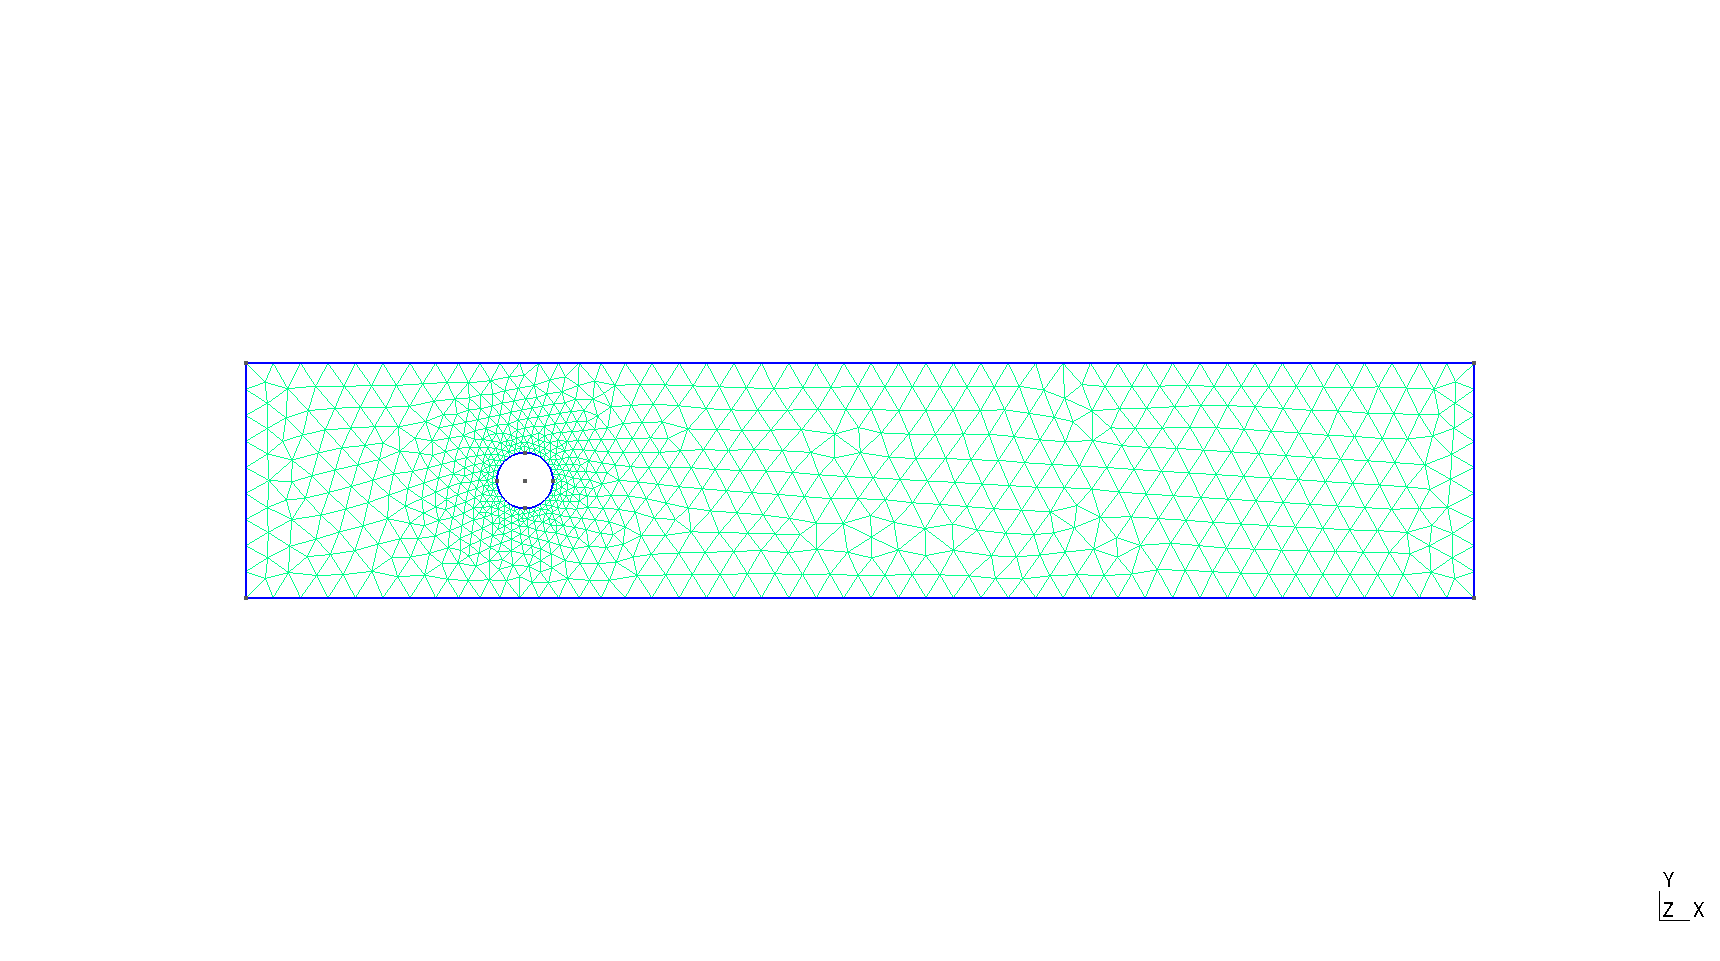
\includegraphics[width=0.45\textwidth]{mesh2d.png}%
    }
    \hfill
    \subfloat[Gmsh representation of a 3D domain. \label{fig:cyl_mesh}]{%
        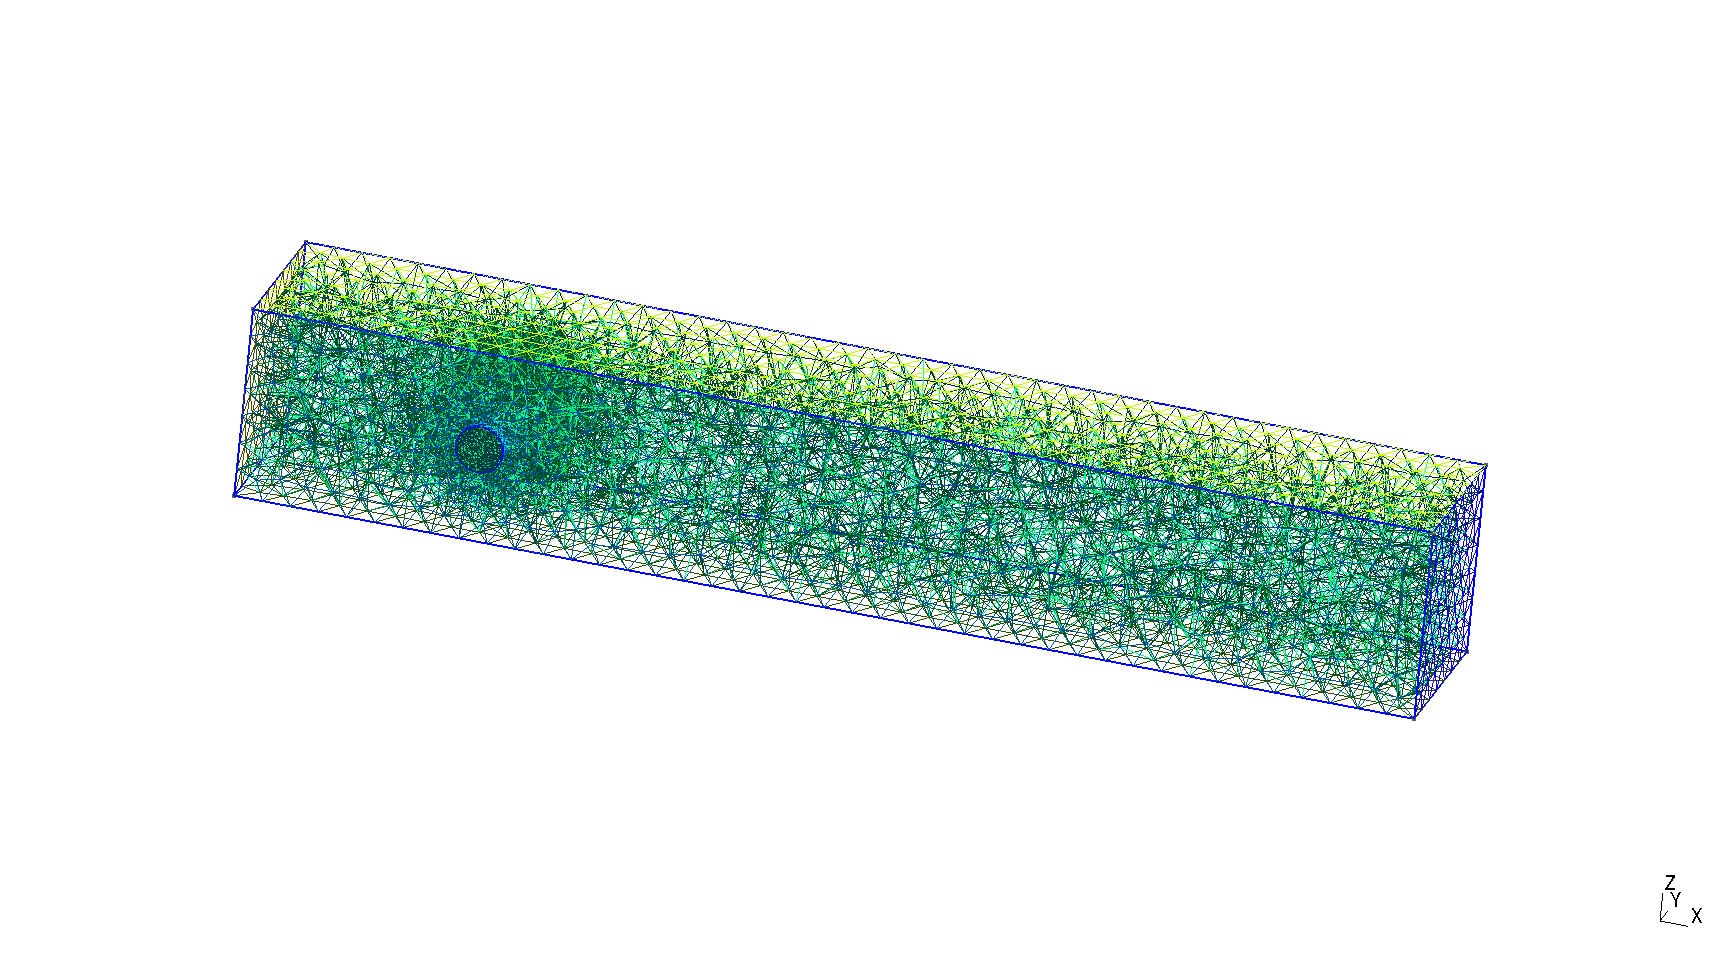
\includegraphics[width=0.45\textwidth]{mesh_cyl.png}%
    }
    \caption{Computational grids generated via \texttt{Gmsh}.}
    \label{fig:mesh_examples}
\end{figure}

The domains were discretised using the Python API of the \texttt{Gmsh} library. This approach allowed for a fully parametric definition of the geometry. To ensure an accurate representation of the physics, the meshing process was dynamically controlled using distance parameters which automatically refined the local grid resolution in critical regions—such as the obstacles layers. In the case of Figure \ref{fig:mesh2d}, the mesh refines in proximity of the circle and gradually gets coarser as soon as the distance increases. A similar approach is shown in Figure \ref{fig:cyl_mesh} as well, where a solid cylindrical structure represents the obstacle where the mesh triangulations are finer. This script-based workflow facilitated the automated generation of diverse mesh configurations.

\subsection{Test Cases}
The following test cases serve as benchmark problems for the solver. Originally defined in 1996 by M. Schäfer and S. Turek \cite{Schafer1996}, they have since become a de facto standard for assessing the performance of CFD solvers. 
\subsubsection{2D case}
\noindent To evaluate the flow solver under different kinematic regimes, the previously cited paper proposes different numerical simulations to perform on the following 2D domain (Figure~\ref{fig:2d_domain}).
\begin{center}
% \caption{Geometry of 2D test case, along with boundary conditions} TODO: How to properly add captions??
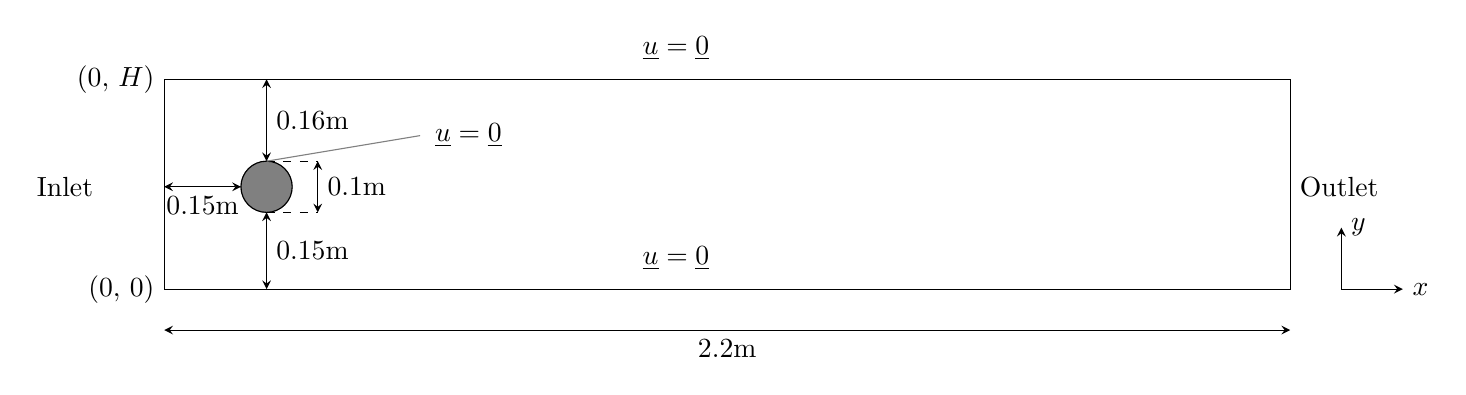
\begin{tikzpicture}[scale=6.5,>=stealth]

% Geometry constants
\def\H{0.41}          % total height (0.15 + 0.16 + 0.15)
\def\L{2.2}           % total length

% Draw outer rectangle
\draw (0,0) rectangle (\L,\H);

% Cylinder
\def\cx{0.20}         % x-position center
\def\cy{0.20}         % y-position center (half of total height)
\def\r{0.05}          % radius

\filldraw[gray] (\cx,\cy) circle (\r);
\draw (\cx,\cy) circle (\r);

% Distances around cylinder
\draw[<->] (\cx,\cy+\r) -- (\cx,\H) node[midway,right] {0.16m};


\draw[<->] (\cx,0) -- (\cx,\cy-\r) node[midway,right] {0.15m};
\draw[<->] (0,\cy) -- (\cx-\r,\cy) node[midway,below] {0.15m};

% Label cylinder diameter
\draw[dashed] (\cx, \cy - \r) -- (\cx + 2*\r, \cy - \r);
\draw[dashed] (\cx, \cy + \r) -- (\cx + 2*\r, \cy + \r);
\draw[<->] (\cx+ 2*\r,\cy-\r) -- (\cx + 2*\r,\cy+\r)
    node[midway,right] {0.1m};

% Labels top and bottom walls
\node at (1.0,\H+0.06) {$\vec{u} = \vec{0}$};
\node at (1.0,+0.06) {$\vec{u} = \vec{0}$};

% Arrow showing inlet direction
\node[left] at (-0.12,\cy) {Inlet};

% Outlet text
\node[right] at (\L,\cy) {Outlet};

% Point coordinate labels
\node[left] at (0,0) {$(0, \, 0)$};
\node[left] at (0,\H) {$(0, \, H)$};

% Total length label
\draw[<->] (0,-0.08) -- (\L,-0.08)
    node[midway,below] {2.2m};

% Coordinate axes
\draw[->] (\L+0.1,0) -- ++(0.12,0) node[right] {$x$};
\draw[->] (\L+0.1,0) -- ++(0,0.12) node[right] {$y$};

% Boundary condition on the cylinder
\draw[-, black!50](\cx, \cy + \r) -- (\cx + 0.3, \cy + 2*\r);
\node[right] at (\cx + 0.31, \cy + 2*\r) {$\vec{u} = \vec{0}$};

\end{tikzpicture}
\captionof{figure}{Geometry of 2D test cases with boundary conditions.}
\label{fig:2d_domain}
\end{center}

 The fluid enters the channel through the inlet boundary with a prescribed velocity profile, while no-slip conditions ($u=v=0$) are imposed on the top and bottom walls, as well as on the cylinder surface. Three distinct test cases were investigated, characterized by the mean inlet velocity $\bar{U}$:

\begin{itemize}
    \item \textbf{Test Case 1 (Low-Re Steady):} A constant low mean velocity of $\bar{U} = 0.3\,\text{m/s}$. This configuration corresponds to a laminar flow regime, expected to produce steady wake patterns.
    
    \item \textbf{Test Case 2 (High-Re Steady):} A constant increased mean velocity of $\bar{U} = 1.5\,\text{m/s}$. In this regime, the Reynolds number is significantly higher, resulting in a more turbulent behaviour.
    
    \item \textbf{Test Case 3 (High-Re Pulsatile):} A time-dependent inflow where the mean velocity $\bar{U} = 1.5\,\text{m/s}$ is modulated by a sinusoidal factor. This introduces a transient forcing frequency to the system, defined as:
    \begin{equation}
    \label{eq:inlet_velocity_2D}
        U_{in}(t) = 4 \cdot \bar{U} \cdot (H - y) \cdot y \cdot\left[\sin(\pi t/8  )  \right] / H^2
    \end{equation}
    where $H$ represents the height of the domain and $y$ the coordinate along the y-axis.
\end{itemize}

\subsubsection{3D cases}
\noindent The investigation was subsequently extended to a three-dimensional domain to capture span-wise flow features and three-dimensional instabilities. The geometry was generated taking inspiration from the M. Schäfer and S. Turek benchmark \cite{Schafer1996}, both an obstacle with square section (Figure~\ref{fig:3d_domain_parallelepiped}) and circular square section (Figure~\ref{fig:3d_domain_cylinder}) have been employed. \\

Consistent with the 2D setup, no-slip conditions were applied to the cylinder and channel walls, while appropriate boundary conditions were imposed on the lateral surfaces to mimic an infinite span or confined channel. The simulation campaign consisted of three test cases:

\begin{itemize}
    \item \textbf{Test Case 1 (Low-Re Steady):} A constant mean inflow velocity of $\bar{U} = 0.45\,\text{m/s}$. This regime serves as a validation baseline, where the flow is expected to remain predominantly laminar and two-dimensional.

    \item \textbf{Test Case 2 (High-Re Steady):} A constant mean inflow velocity of $\bar{U} = 2.25\,\text{m/s}$. At this higher Reynolds number, the flow transitions to a three-dimensional state.

    \item \textbf{Test Case 3 (High-Re Unsteady):} A time-varying inflow with a mean velocity of $\bar{U} = 2.25\,\text{m/s}$, modulated by a sinusoidal profile. In this case a transient forcing frequency to the system was added, defined as:
    \begin{equation}
    \label{eq:inlet_velocity_3D}
        U_{in}(t) = 16 \cdot \bar{U} \cdot (H - y) \cdot (W - z) \cdot y \cdot z \cdot\left[\sin(\pi t/8  )  \right] / H^4
    \end{equation}
    where $H$ represents the height of the domain, $W$ the width of the domain and ($y$, $z$) the coordinate along the y and z axis.
\end{itemize}

\begin{center}
%TODO: What wrong choices in my life led me to use tikz for such complex images???
% This is something actually impressive I must admit (TG)
    \begin{tikzpicture}[tdplot_main_coords, font=\small, scale=7.5, >=stealth]
    
        % --- 1. Dimensions (Mapped to TikZ: x=width, y=length, z=height) ---
        \def\W{0.41}    % Width 
        \def\L{2.5}     % Length 
        \def\H{0.41}    % Height 
        
        \def\obsW{0.41}  
        \def\obsL{0.1} 
        \def\obsH{0.1}  
        
        % Positioning
        \def\obsXstart{0} % Centered in x
        \def\obsYstart{0.45}   % Gap from inflow 
        \def\obsZstart{0.15}  % Height from bottom 
    
        % --- 2. Hidden Lines (Back of Domain) ---
        \draw[dashed] (0,\L,0) -- (\W,\L,0);
        \draw[dashed] (0,0,0) -- (0,\L,0);
        \draw[dashed] (0,\L,0) -- (0,\L,\H);
    
        % --- 3. The Obstacle  ---
        % The order in which the faces are drawn matters, should be changed in case of change of perspecitive
        % 1. Back face 
        \filldraw[fill=gray!80] (\obsXstart,\obsYstart,\obsZstart) -- ++(\obsW,0,0) -- ++(0,0,\obsH) -- ++(-\obsW,0,0) -- cycle;
        
        % 2. Left side face 
        \filldraw[fill=gray!70] (\obsXstart,\obsYstart,\obsZstart) -- ++(0,\obsL,0) -- ++(0,0,\obsH) -- ++(0,-\obsL,0) -- cycle;
        
        % 3. Bottom face 
        \filldraw[fill=gray!90] (\obsXstart,\obsYstart,\obsZstart) -- ++(\obsW,0,0) -- ++(0,\obsL,0) -- ++(-\obsW,0,0) -- cycle;
        
        % 4. Right side face 
        \filldraw[fill=gray!50] (\obsXstart+\obsW,\obsYstart,\obsZstart) -- ++(0,\obsL,0) -- ++(0,0,\obsH) -- ++(0,-\obsL,0) -- cycle;
    
        % 5. Top face 
        \filldraw[fill=gray!20] (\obsXstart,\obsYstart,\obsZstart+\obsH) -- ++(\obsW,0,0) -- ++(0,\obsL,0) -- ++(-\obsW,0,0) -- cycle;
    
        % 6. Front face 
        \filldraw[fill=gray!40] (\obsXstart,\obsYstart,\obsZstart) -- ++(\obsW,0,0) -- ++(0,0,\obsH) -- ++(-\obsW,0,0) -- cycle;
    
        % --- 4. Main Domain Wireframe ---
        % Inflow Plane (y=0 in TikZ)
        \draw (0,0,0) -- (\W,0,0) -- (\W,0,\H) -- (0,0,\H) -- cycle;
        % Outflow Plane (y=L in TikZ, only nondashed lines)
        \draw (\W,\L,0) -- (\W,\L,\H) -- (0,\L,\H);
        % Connecting Edges
        \draw (\W,0,0) -- (\W,\L,0);
        \draw (\W,0,\H) -- (\W,\L,\H);
        \draw (0,0,\H) -- (0,\L,\H);
    
        % --- 5. Dimension Labels ---
        % Total Length
        \draw[<->, gray] (\W-0.1, 0, \H) -- node[above] {2.5m} (\W-0.1, \L, \H);
        
        % Inflow dimensions
        \draw[dashed, gray] (0, 0, 0) -- (0, -0.08, 0);
        \draw[dashed, gray] (\W, 0, 0) -- (\W, -0.08, 0);
        \draw[dashed, gray] (0, 0, \H) -- (0, -0.08, \H);
        \draw[<->, gray] (0, -0.08, 0) -- node[below] {0.41m} (\W, -0.08, 0);
        \draw[<->, gray] (0, -0.08, 0) -- node[left] {0.41m} (0, -0.08, \H);
    
        % Obstacle Height Stack
        \draw[<->, gray] (\obsXstart, \obsYstart, 0) -- node[left] {0.15m} (\obsXstart, \obsYstart, \obsZstart);
        \draw[dashed, gray] (\obsXstart, \obsYstart, \obsZstart) -- (\obsXstart, \obsYstart-0.08, \obsZstart);
        \draw[dashed, gray] (\obsXstart, \obsYstart, \obsZstart+\obsH) -- (\obsXstart, \obsYstart-0.08, \obsZstart+\obsH);
        \draw[<->, gray] (\obsXstart, \obsYstart-0.08, \obsZstart) -- node[left] {0.1m} (\obsXstart, \obsYstart-0.08, \obsZstart+\obsH);
        \draw[<->, gray] (\obsXstart, \obsYstart, \obsZstart+\obsH) -- (\obsXstart, \obsYstart, \H);
        \node[anchor = north west, gray] at (\obsXstart, \obsYstart, \H){0.16m};
    
        % Obstacle Length and downstream gap
        \draw[<->, gray] (\obsXstart+\obsW, \obsYstart, \obsZstart) -- (\obsXstart+\obsW, 0, \obsZstart);
        \node[anchor=south west, gray] at (\obsXstart+\obsW, 0, \obsZstart+0.018) {0.45m};
        \draw[<->, gray] (\obsXstart+\obsW, \obsYstart+\obsL, \obsZstart) -- node[above] {1.95m} (\obsXstart+\obsW, \L, \obsZstart);
        \draw[dashed, gray] (\obsXstart+\obsW, \obsYstart, \obsZstart + \obsH) -- (\obsXstart+\obsW, \obsYstart, \obsZstart + \obsH+0.07);
        \draw[dashed, gray] (\obsXstart+\obsW, \obsYstart + \obsL, \obsZstart + \obsH) -- (\obsXstart+\obsW, \obsYstart + \obsL, \obsZstart + \obsH+0.07);
        \draw[<->, gray] (\obsXstart+\obsW, \obsYstart, \obsZstart + \obsH+0.07) -- node[above] {0.1m} (\obsXstart+\obsW, \obsYstart + \obsL, \obsZstart + \obsH+0.07);
    
        % --- 6. Boundary Condition Text ---
        \node[anchor=north east] at (0,-0.03,0) {(0,0,0)};
        \node[anchor=south east] at (0,0,\H) {(0,H,0)};
        \node[anchor=north west] at (\W,0,0) {(0,0,H)};
        
        \node at (\W/2-0.1, 0, -0.1) {Inlet};
        \node[anchor=south east] at (\W+0.1, \L, \H+0.1) {Outlet};
    
        \draw[->] (\W/2-0.015, \L/2-0.015, \H+0.09) -- (\W/2, \L/2, \H);
        \draw[->, dashed] (\W/2-0.015, \L/2-0.015, \H+0.09) -- (\W/2, \L-0.4, \H/2);
        \node[anchor=south] at (\W/2-0.015, \L/2-0.015, \H+0.09) {$\vec{u} = \vec{0}$};
        \draw[->, dashed] (\W/2, \L/2, -0.09) -- (\W/2, \L/2, 0);
        \draw[->] (\W/2, \L/2, -0.09) -- (\W/2, \L-0.4, 0);
        \node[anchor=north] at (\W/2, \L/2, -0.09) {$\vec{u} = \vec{0}$};
        \draw[->] (\obsXstart+\obsW/2, \obsYstart+\obsL+0.4, \obsZstart+\obsH/2) -- (\obsXstart+\obsW/2, \obsYstart + \obsL, \obsZstart+\obsH/2 -0.05);
        \node[anchor=south] at (\obsXstart+\obsW/2, \obsYstart+\obsL+0.4, \obsZstart+\obsH/2) {$\vec{u} = \vec{0}$};
    
        % --- 7. Axis Legend (Matches image coordinate system) ---
        \begin{scope}[shift={(\W+0.1, \L-0.25, -0.4)}]
            \draw[->, thick] (0,0,0) -- (0.3,0,0) node[anchor=north east] {z};
            \draw[->, thick] (0,0,0) -- (0,0.3,0) node[anchor=north west] {x};
            \draw[->, thick] (0,0,0) -- (0,0,0.3) node[anchor=south] {y};
        \end{scope}
    
    \end{tikzpicture}
\captionof{figure}{Geometry of 3D test cases with boundary conditions for flow around an obstacle with square section ("parallelepiped").}
\label{fig:3d_domain_parallelepiped}
\end{center}

\begin{center}
    \begin{tikzpicture}[tdplot_main_coords, font=\small, scale=7.5, >=stealth]
    
        % --- 1. Dimensions ---
        \def\W{0.41}    % Width 
        \def\L{2.5}     % Length 
        \def\H{0.41}    % Height 
        
        % Obstacle Parameters (Cylinder)
        \def\obsD{0.1}          
        \def\obsR{0.05}         % Radius (Diameter 0.1)
        \def\obsYstart{0.45}    % Gap from inflow 
        \def\obsZstart{0.15}    % Height from bottom 
        
        % Derived Centers
        \def\yc{\obsYstart + \obsR}
        \def\zc{\obsZstart + \obsR}
        \def\obsXstart{0} 
    
        % --- 2. Hidden Lines (Back of Domain) ---
        \draw[dashed] (0,\L,0) -- (\W,\L,0);
        \draw[dashed] (0,0,0) -- (0,\L,0);
        \draw[dashed] (0,\L,0) -- (0,\L,\H);
    
        % --- 3. The Obstacle (Cylinder) ---
        
        % A. The curved surface (Hull) - Facing the viewer/Inlet
        % We draw from top-left, to top-right, arc around the front to bottom-right, then back to bottom-left.
        \filldraw[fill=gray!25, draw=black] 
            (0, \yc, \zc+\obsR)               % 1. Top-Left point
            -- (\W, \yc, \zc+\obsR)           % 2. Top-Right point
            -- plot[domain=90:270, variable=\t] ({\W}, {\yc + \obsR*cos(\t)}, {\zc + \obsR*sin(\t)}) % 3. Right Arc (Front side)
            -- (0, \yc, \zc-\obsR)            % 4. Bottom-Left point
            -- plot[domain=270:90, variable=\t] ({0}, {\yc + \obsR*cos(\t)}, {\zc + \obsR*sin(\t)})  % 5. Left Arc (Front side)
            -- cycle;
    
        % B. The Right End Cap (Circular Face) - DARK GRAY
        \filldraw[fill=gray!70, draw=black] plot[domain=0:360, variable=\t] ({\W}, {\yc + \obsR*cos(\t)}, {\zc + \obsR*sin(\t)});
        
        % C. Definition Lines (Edges for clarity)
        \draw[black] (0, \yc, \zc+\obsR) -- (\W, \yc, \zc+\obsR); % Top tangent
        \draw[black] (0, \yc, \zc-\obsR) -- (\W, \yc, \zc-\obsR); % Bottom tangent
    
        % --- 4. Main Domain Wireframe ---
        \draw (0,0,0) -- (\W,0,0) -- (\W,0,\H) -- (0,0,\H) -- cycle;
        \draw (\W,\L,0) -- (\W,\L,\H) -- (0,\L,\H);
        \draw (\W,0,0) -- (\W,\L,0);
        \draw (\W,0,\H) -- (\W,\L,\H);
        \draw (0,0,\H) -- (0,\L,\H);
    
        % --- 5. Dimension Labels ---
        % Total Length
        \draw[<->, gray] (\W-0.1, 0, \H) -- node[above] {2.5m} (\W-0.1, \L, \H);
        
        % Inflow dimensions
        \draw[dashed, gray] (0, 0, 0) -- (0, -0.08, 0);
        \draw[dashed, gray] (\W, 0, 0) -- (\W, -0.08, 0);
        \draw[dashed, gray] (0, 0, \H) -- (0, -0.08, \H);
        \draw[<->, gray] (0, -0.08, 0) -- node[below] {0.41m} (\W, -0.08, 0);
        \draw[<->, gray] (0, -0.08, 0) -- node[left] {0.41m} (0, -0.08, \H);
    
        % Obstacle Height Stack
        \draw[<->, gray] (\obsXstart, \yc, 0) -- node[left] {0.15m} (\obsXstart, \yc, \zc-\obsR);
        \draw[dashed, gray] (\obsXstart, \yc-\obsR, \zc-\obsR) -- (\obsXstart, \yc-0.13, \zc-\obsR);
        \draw[dashed, gray] (\obsXstart, \yc-\obsR, \zc+\obsR) -- (\obsXstart, \yc-0.13, \zc+\obsR);
        \draw[<->, gray] (\obsXstart, \yc-0.13, \zc-\obsR) -- node[left] {0.1m} (\obsXstart, \yc-0.13, \zc+\obsR);
        \draw[<->, gray] (\obsXstart, \yc, \zc+\obsR) -- (\obsXstart, \yc, \H);
        \node[anchor = north west, gray] at (\obsXstart, \yc, \H){0.16m};
    
        % Obstacle Location (Streamwise)
        \draw[<->, gray] (\obsXstart+\W, \yc-\obsR, \zc) -- (\obsXstart+\W, 0, \zc);
        \node[anchor=north west, gray] at (\obsXstart+\W, 0, \zc+0.018) {0.45m};
        
        \draw[<->, gray] (\obsXstart+\W, \yc+\obsR, \zc) -- node[above] {1.95m} (\obsXstart+\W, \L, \zc);
        
        % Diameter Label (Top)
        \draw[dashed, gray] (\obsXstart+\W, \yc-\obsR, \zc + \obsR) -- (\obsXstart+\W, \yc-\obsR, \zc + \obsR+0.07);
        \draw[dashed, gray] (\obsXstart+\W, \yc+\obsR, \zc + \obsR) -- (\obsXstart+\W, \yc+\obsR, \zc + \obsR+0.07);
        \draw[<->, gray] (\obsXstart+\W, \yc-\obsR, \zc + \obsR+0.07) -- node[above] {0.1m} (\obsXstart+\W, \yc+\obsR, \zc + \obsR+0.07);
    
        % --- 6. Boundary Conditions ---
        \node[anchor=north east] at (0,-0.03,0) {(0,0,0)};
        \node[anchor=south east] at (0,0,\H) {(0,H,0)};
        \node[anchor=north west] at (\W,0,0) {(0,0,H)};
        
        \node at (\W/2-0.1, 0, -0.1) {Inlet};
        \node[anchor=south east] at (\W+0.1, \L, \H+0.1) {Outlet};
    
        % Velocity Vectors
        \draw[->] (\W/2-0.015, \L/2-0.015, \H+0.09) -- (\W/2, \L/2, \H);
        \draw[->, dashed] (\W/2-0.015, \L/2-0.015, \H+0.09) -- (\W/2, \L-0.4, \H/2);
        \node[anchor=south] at (\W/2-0.015, \L/2-0.015, \H+0.09) {$\vec{u} = \vec{0}$};
        
        \draw[->, dashed] (\W/2, \L/2, -0.09) -- (\W/2, \L/2, 0);
        \draw[->] (\W/2, \L/2, -0.09) -- (\W/2, \L-0.4, 0);
        \node[anchor=north] at (\W/2, \L/2, -0.09) {$\vec{u} = \vec{0}$};
        
        % Cylinder BC
        \draw[->] (\obsXstart+\W/2, \yc+\obsR+0.4, \zc) -- (\obsXstart+\W/2, \yc+\obsR, \zc);
        \node[anchor=south] at (\obsXstart+\W/2, \yc+\obsR+0.4, \zc) {$\vec{u} = \vec{0}$};
    
        % --- 7. Axis Legend ---
        \begin{scope}[shift={(\W+0.1, \L-0.25, -0.4)}]
            \draw[->, thick] (0,0,0) -- (0.3,0,0) node[anchor=north east] {z};
            \draw[->, thick] (0,0,0) -- (0,0.3,0) node[anchor=north west] {x};
            \draw[->, thick] (0,0,0) -- (0,0,0.3) node[anchor=south] {y};
        \end{scope}
    
    \end{tikzpicture}
    \captionof{figure}{Geometry of 3D test cases with boundary conditions for flow around an obstacle with circular section ("cylinder").}
    \label{fig:3d_domain_cylinder}
\end{center}

\subsection{Drag-Lift coefficients}

The computation of drag-lift coefficients is required during the simulation of all test cases and defined as followed:
\begin{equation}
\label{eq:drag_lift_coeff}
    C_D = \frac{F_D}{\bar{U}^2 A} \qquad \wedge \qquad C_L = \frac{F_L}{\bar{U}^2 A},
\end{equation}
where $F_D$ (parallel to the flow direction) and $F_L$ (perpendicular to the the flow direction) are the corresponding forces applied on the object, $\bar{U}$ is the mean velocity and $A$ is the characteristic area ($D$ for \textbf{2D}, $D \cdot H$ for \textbf{3D}) 

In particular, those are non-dimensional quantities used to measure the aerodynamic force acting on the cylinder placed inside the channel.

Before diving into the definition of the forces, we need to introduce the definition of \textbf{Stress Tensor} $\sigma$ whose formula is the following:

\begin{equation*}
    \sigma = -p\text{I} + \mu (\nabla \vec{u} + (\nabla \vec{u})^T)
\end{equation*}
where $p$ is the pressure, $\text{I}$ is the identity matrix, $\mu$ (or $p\nu$) is the dynamic viscosity, $\nabla \vec{u} + (\nabla \vec{u})^T$ is the rate of strain tensor.

\vspace{5mm}

The total force vector $\vec{F}$ acting on the obstacle is the surface integral of the stress tensor dotted with the normal vector $\hat{\eta}$ (pointing out of the fluid and into the obstacle):

\begin{equation*}
    \vec{F} = \int_{S} \boldsymbol{\sigma} \cdot \hat{\eta} \, dS 
\end{equation*}

The Drag force ($F_D$) and Lift force ($F_L$) are defined as the components of the total force vector $\vec{F}$ parallel and perpendicular to the flow direction, respectively. Assuming the flow is aligned with the x-axis:

\begin{equation}
\label{eq:drag_lift_forces}
    F_D = F_x \quad \quad F_L = F_y
\end{equation}


\section{Description of the Solver}
The computational framework is built upon the \texttt{deal.II} finite element library, which handles mesh management and Degrees of Freedom (\textit{DoFs}) distribution. For the linear algebra, which in particular refers to the parallel distribution of the solver and the use of preconditioners, we utilized the \texttt{Trilinos} library. The solution procedure follows a nonlinear Newton iteration loop to linearize the convective term. The Jacobian systems obtained at each Newton step are solved using the GMRES algorithm. To verify the correctness of the implementation, we conducted convergence studies and flow analysis on three specific benchmarks, performing simulations for both 2D and 3D geometries. In addition to that, several preconditioners where used, in order to obtain a better conditioning in the linear systems' matrices.
\subsection{Parameters Setting}
In \texttt{main} function parameters are parsed to configure the problem setup. While the temporal parameters are fixed, the physical properties and geometry can be controlled via the command-line flags listed in Table~\ref{tab:cli_args}.

\begin{table}[h!]
    \centering
    \begin{tabular}{l l l}
        \toprule
        \textbf{Flag} & \textbf{Variable} & \textbf{Description} \\
        \midrule
        \texttt{-f} & \texttt{mesh\_file\_name} & Path to the Gmsh grid file (.msh) \\
        \texttt{-v} & $\nu$ (viscosity) & Kinematic viscosity of the fluid \\
        \texttt{-u} & $U_{max}$ & Max inflow velocity \\
        \texttt{-theta} & $\theta$ & Time-stepping parameter (suggested 0.5 or 1.0) \\
        \texttt{-d} & $d$ (dim) & Spatial dimension (2 or 3) \\
        \texttt{-T} & $T_{end}$ & Total simulation time \\
        \texttt{-dt} & $\Delta t$ & Time step size \\
        \texttt{-td} & $time\_dependency$ & Allows to choose between inlet conditions \eqref{eq:inlet_velocity_3D}/\eqref{eq:inlet_velocity_2D} \\
        & & or ramped parabolic inlet velocity \\
        \bottomrule
    \end{tabular}
    \caption{Command-line arguments available for simulation configuration.}
    \label{tab:cli_args}
\end{table}

If not specified, parameters follow their default initialization:
\begin{lstlisting}[language=C++]
    // default settings
    std::string mesh_file_name = "../mesh/mesh3D_example.msh";
    double viscosity = 1.0;
    double theta = 1.0; // Backward Euler
    double U_max = 0.45;
    int dim = 3;
    double T = 2.;              
    double delta_t = 0.02;
\end{lstlisting}
\captionof{lstlisting}{Configuration of simulation parameters.}

Depending on the provided dimension flag, the code instantiates the solver for either 2D or 3D domains and initiates the \texttt{run\_time\_simulation} routine.

\subsection{System Initialization}
The initialization phase is handled by the \texttt{initialize\_system} function, which first constructs the parallel grid by reading a Gmsh format file and partitioning the \texttt{Triangulation} across the available MPI processes. 

The finite element space is built using \texttt{FE\_SimplexP} basis functions, combining the velocity and pressure fields into a single coupled \texttt{FESystem}. To ensure the numerical stability of the system arising from the incompressibility constraint, the finite element spaces were chosen to satisfy the Ladyzhenskaya-Babuška-Brezzi (LBB) inf-sup condition \ref{eq:lbb_condition}. We adopted the stable Taylor-Hood element pair ($\mathbb{P}^{2}/\mathbb{P}^{1}$). This choice suppresses spurious pressure modes and guarantees optimal convergence rates for both variables. 

The block sparsity patterns are generated by defining the specific coupling between velocity and pressure degrees of freedom. Finally, all distributed vectors including the solution, Newton update, and right hand side are reinitialized using \texttt{TrilinosWrappers} based on the locally owned degrees of freedom.

\subsection{System Assemble}
The assembly of the linear system is performed within the \texttt{assemble} function, which iterates over all locally owned cells to construct both the Jacobian matrix and the residual vector. For each cell, we initialize \texttt{FEValues} objects to evaluate the shape functions, gradients, and quadrature weights. The implementation distinguishes between the system matrix assembly (controlled by the \texttt{assemble\_matrix} flag) and the right-hand side.

During the matrix assembly, we construct the Jacobian of the non-linear residual. This includes the mass matrix contribution from the time derivative ($\frac{1}{\Delta t}$), the viscous diffusion term ($\theta \nu (\nabla \vec{u}, \nabla \vec{v})$), and the linearized convective term. An auxiliary \texttt{cell\_pressure\_mass\_matrix} is assembled for the following initialization of a block preconditioner.

The RHS vector (\texttt{local\_rhs}) accumulates the residual of the weak formulation. The time integration follows a $\theta$ scheme. Boundary conditions are handled by identifying faces on the outlet boundary (ID 2); here, a traction term $-p_{out} \hat{\eta} \cdot \vec{v}$ is integrated using \texttt{FEFaceValues}.

Finally, the local contributions are distributed to the global system using \texttt{AffineConstraints}. A critical distinction is made here: if \texttt{initial\_step} is true, we apply inhomogeneous boundary constraints (\texttt{nonzero\_constraints}); otherwise, for Newton updates, we apply homogeneous constraints (\texttt{zero\_constraints}) to solving for the increment $\delta \vec{u}$.

\subsection{Newton Iteration}
As already stated in the introduction of the section, the non-linear problem is solved using a Newton-Raphson iterative scheme. At each step $k$, we calculate the Newton update $\delta \vec{u}$ by solving the linearized system:
\begin{equation*}
    J(\vec{u}_k) \delta \vec{u} = -\vec{R}(\vec{u}_k)
\end{equation*}
where $J$ is the Jacobian matrix and $\vec{R}$ is the residual vector. To ensure global convergence, specifically when the initial guess is far from the solution, we employ a backtracking line search strategy. If a Newton step fails to reduce the residual enough below the tolerance, the damping factor $\alpha$ is halved at each iteration and the update is computed again:
\begin{equation*}
    \alpha \leftarrow 0.5\alpha
\end{equation*}
This process repeats until the monotonicity condition is satisfied:
\begin{equation*}
    \|\vec{R}(\vec{u}_k + \alpha \delta \vec{u})\| < \|\vec{R}(\vec{u}_k)\|
\end{equation*}
Within each Newton step, the linear system is inverted using the Flexible Generalized Minimal Residual method (FGMRES), provided by the \texttt{Trilinos} framework.

\subsection{Drag and Lift Coefficients}

The computation of the aerodynamic coefficients is performed within the \texttt{compute\_lift\_drag} function. This procedure is executed as a post-processing step at the end of each time step, once the Newton solver has successfully converged.

The solver computes the total force vector $\vec{F}$ acting on the cylinder by integrating the stress tensor $\sigma$ over the cylinder's surface $S$.
Since the code can't computationally solve the integral in a continuous domain, we used the \textbf{Gaussian Quadrature}, which transforms the integral into a finite summation over discrete quadrature points, to approximate it.

The implementation utilizes the \texttt{FEFaceValues} class from the \texttt{deal.II} library to evaluate shape functions and gradients on the boundary. 

The algorithm proceeds through the following steps: 
\begin{enumerate} 
    \item \textbf{Boundary Iteration:} The solver iterates through all locally owned active cells \texttt{dof\_handler.active\_cell\_iterators()} to identify faces located on the cylinder boundary. 
    \item \textbf{Stress Reconstruction:} At each quadrature point, the local pressure \texttt{p\_val} and velocity gradients \texttt{grad\_u} are extracted. These are used to reconstruct the viscous stress tensor \texttt{stress}. 
    \item \textbf{Force Accumulation:} The stress tensor is contracted with the outward normal vector n to obtain the local force density. This density is multiplied by the \texttt{JxW} term and accumulated into the \texttt{total\_force} vector. 
\end{enumerate}

Once the accumulation of forces is complete, the code sums the forces across all MPI processes and stores the final result in the local vector \texttt{global\_force}.

Finally, the total force is normalized by the square of the reference velocity and the reference length to derive the drag ($C_D$) and lift ($C_L$) coefficients, which are computed from the accumulated \texttt{global\_force[0]} and \texttt{global\_force[1]}, respectively.

\subsection{Preconditioners}

To enhance performance, the solver employs preconditioning techniques to speed up convergence, which leads significant improvements in terms of iterations, and it avoids convergence failures during the simulation. Since the linear system arising from the Navier-Stokes equations is of the saddle-point type, standard black-box preconditioners often fail; therefore, we implement physics-based block preconditioners that exploit the $2 \times 2$ block structure of the system matrix:

\begin{equation}
    \mathcal{A} = 
    \begin{pmatrix} 
    A & B^T \\ 
    B & 0 
    \end{pmatrix}
\end{equation}
where $A$ represents the velocity stiffness matrix (including time, convective, and viscous terms), and $B$ and $B^T$ represent the divergence and gradient operators, respectively.

In the following 

\subsubsection{Block Diagonal Preconditioner}

The simplest approach implemented is the Block Diagonal Preconditioner (class \texttt{BlockPreconditioner}), which doesn't consider the coupling between velocity and pressure fields. The preconditioning matrix $\mathcal{P}_{diag}$ is defined as:
\begin{equation}
    \mathcal{P}_{diag}^{-1} = 
    \begin{pmatrix} 
    \tilde{A}^{-1} & 0 \\ 
    0 & \tilde{M_p}^{-1} 
    \end{pmatrix}
\end{equation}
In our implementation, the inverses $\tilde{A}^{-1}$ and $\tilde{M_p}^{-1}$ are approximated by solving the respective blocks using the \textbf{Conjugate Gradient} (CG) method preconditioned with an \textbf{Incomplete LU} (ILU) factorization. Despite of its simple implementation, this preconditioner is generally less robust for non-stationary flows with significant time-dependency.

\subsubsection{Block Triangular Preconditioner}

The Block Triangular Preconditioner (class \texttt{PreconditionBlockTriangular}) improves upon the diagonal approach by accounting for the one-way coupling from velocity to pressure. It approximates the system using a lower triangular form:
\begin{equation}
    \mathcal{P}_{tri} = 
    \begin{pmatrix} 
    A & 0 \\ 
    B & M_p 
    \end{pmatrix}
\end{equation}
The application of this preconditioner involves a two-step process:
\begin{enumerate}
    \item \textbf{Velocity Solve:} Solve $A \vec{u} = \vec{f}$ using \textbf{GMRES} with \textbf{ILU preconditioning}.
    \item \textbf{Pressure Solve:} Update the pressure residual $\vec{r}_p = \vec{g} - B\vec{u}$ and solve $M_p \vec{p} = \vec{r}_p$ using \textbf{CG} with \textbf{ILU preconditioning}.
\end{enumerate}

\subsubsection{Schur Complement Preconditinoner}

The most strategical preconditioner employed is the Block Schur Preconditioner (class \texttt{BlockSchurPreconditioner}), which is the currently active method in the solver. This approach utilizes the \textbf{Upper Triangular factorization}of the block system:
\begin{equation}
    \mathcal{P}_{Schur}^{-1} = 
    \begin{pmatrix} 
    A & B^T \\ 
    0 & S 
    \end{pmatrix}^{-1}
\end{equation}
where $S = -B A^{-1} B^T$ is the Schur complement. Since calculating $S$ explicitly is computationally expensive, we approximate it using the pressure mass matrix scaled by the viscosity $\nu$ and the time-stepping coefficient $\gamma$ (where $\gamma \propto 1/\Delta t$). The approximation used is:
\begin{equation}
    \tilde{S}^{-1} \approx -(\nu + \gamma) M_p^{-1}
\end{equation}
The application of this preconditioner proceeds as follows:
\begin{enumerate}
    \item \textbf{Pressure Predictor:} Solve the approximated Schur system for pressure: $M_p \vec{p} = -(\nu + \gamma)^{-1} \vec{g}$. This is performed using \textbf{FGMRES} on the pressure mass matrix.
    \item \textbf{Velocity Update:} Compute the velocity residual $\vec{r}_u = \vec{f} - B^T \vec{p}$ and solve $A \vec{u} = \vec{r}_u$ using \textbf{ILU factorization}.
\end{enumerate}
This method effectively handles the saddle-point nature of the problem, providing the most stability for the Reynolds numbers considered in this study. 

\subsection{Output}
The visualization of results is managed by a function which uses the \texttt{DataOut} class to export the finite element solution of each time istant. The solution vector is decomposed into its physical components, with velocity interpreted as a vector field of dimension $dim$ and pressure as a scalar. Before saving, the Reynolds number is computed based on the domain dimensionality and the inlet mean velocity $U_{mean}$. This value is used to generate dynamic filenames (e.g., \texttt{100Re-NS\_Solution\_...}).

The simulation results were visualized and analyzed using the open-source software \texttt{ParaView}. Since the output data was stored in the parallel VTK format (\texttt{.pvtu}), \texttt{ParaView} automatically reconstructed the global computational domain by aggregating the data fragments from individual MPI processes. The time-dependent evolution of the flow was visualized by loading the sequence of solution files which represented each a single time step.

\section{The Splitting Method of Chorin and Temam}
\label{sec:ChorinTemam}
The Chorin-Temam method is a fractional-step scheme used to decouple the velocity and pressure fields in the incompressible Navier-Stokes equations.
\subsection{Algorithm}
Given the velocity $\vec{u}^{(n)}$ at time $t^{(n)}$, we find $\vec{u}^{(n+1)}$ and $p^{(n+1)}$ through the following steps:
\begin{enumerate}
    \item \textbf{Prediction Step:} Solve for the intermediate velocity field $\tilde{\vec{u}}^{(n+1)}$ by considering convection and diffusion.
    \begin{equation}
        \label{eq:chorin_step_1}
        \left\{ \begin{aligned}
            &\frac{\tilde{\vec{u}}^{(n+1)} - \vec{u}^{(n)}}{\Delta t} - \nu \Delta \tilde{\vec{u}}^{(n+1)} + (\vec{u}^* \cdot \nabla)\vec{u}^{**} = \vec{f}^{(n+1)} && \text{in } \Omega, \\
            &\tilde{\vec{u}}^{(n+1)} = \vec{0} && \text{on } \partial\Omega;
        \end{aligned} \right.
    \end{equation}
    
    \item \textbf{Pressure Poisson Equation:} Solve for the pressure $p^{n+1}$ that will enforce the incompressibility constraint.
    \begin{equation}
        \label{eq:chorin_step_2}
        \left\{ \begin{aligned}
            &\frac{\vec{u}^{(n+1)} - \tilde{\vec{u}}^{(n+1)}}{\Delta t} + \nabla p^{(n+1)} = \vec{0} && \text{in } \Omega, \\
            &\Div \left( \vec{u}^{n+1} \right) = 0 && \text{in } \Omega, \\
            &\vec{u}^{(n+1)} \cdot \hat{\eta} = 0 && \text{on } \partial\Omega,
        \end{aligned} \right.
    \end{equation}
    
    \item \textbf{Projection Step:} Update the velocity field to the next time level using the pressure gradient.

    \begin{tcolorbox}[colback = bluePoli!10, colframe=bluePoli]
    \begin{equation}
        \vec{u}^{(n+1)} = \vec{u}^* - \Delta t \nabla p^{(n+1)}
    \end{equation}
\end{tcolorbox}
\end{enumerate}
\subsection{Convergence}
The Chorin-Temam projection method is widely adopted in computational fluid dynamics (CFD) due to its efficiency in decoupling the velocity and pressure fields. Its behaviour and benefits are briefly described below.

For the classical scheme described above \eqref{eq:chorin_step_1}, the following convergence rates are typically observed:
\begin{itemize}
    \item \textbf{Velocity:} The method achieves first-order accuracy in time, $\mathcal{O}(\Delta t)$, in the $[L^2(\Omega)]^d$ norm.
    \item \textbf{Pressure:} The pressure field generally converges at a rate of $\mathcal{O}(\Delta t^{1/2})$ in the $L^2(\Omega)$ norm, although this can be improved to $\mathcal{O}(\Delta t)$ with incremental variants.
    \item \textbf{Convergence:} Depends by the choice of finite element spaces ($\mathbb{P}^k/\mathbb{P}^{k-1}$), typically $\mathcal{O}(h^{k+1})$ for velocity.
\end{itemize}

\subsection*{Key Points of the Algorithm}
\begin{itemize}
    \item \textbf{Operator Decoupling:} By splitting the momentum and continuity equations, the algorithm avoids solving a large system. Instead, it solves a sequence of simpler elliptic and parabolic problems.
    \item \textbf{Computational Efficiency:} The most expensive part is solving the Pressure Poisson Equation. Since the Laplace operator is symmetric and positive definite, highly efficient solvers like Conjugate Gradient (CG) can be used.
    \item \textbf{Linearization:} The semi-implicit approach $(\vec{u}^{(n)} \cdot \nabla)\vec{u}^*$ eliminates the need for the expensive Newton methods for the non-linear convective term within each time step, which was utilized in the classical solver.
\end{itemize}

\section{Results and discussion}
\subsection{2D test cases}
\subsubsection{2D Test Case 1}

2D Test Case 1 represents a low $\Reynolds$ ($\Reynolds = 20$) simulation in the steady regime. The simulation has been carried out from  $t_{0} = 0 s$ to $T = 5 s$ with a discretization step $\Delta t = 0.02 s$.

Figure~\ref{fig:2d_1_dl} shows the temporal evolution of the drag and lift coefficients. We can identify two main phases in the flow development:
\begin{enumerate}
    \item \textbf{Transient Phase}: At the beginning ($t < 1.5s$), the flow exhibits a startup transient. The drag coefficient shows a sharp initial overshoot (peak of approximately 7.3) on the fine mesh. The lift coefficient exhibits a distinct oscillation before convergence
    \item \textbf{Steady Phase}: After the previous phase ($t \ge 1.5s$), the flow converges into a stable state. Both drag and lift coefficients converge to their corresponding constant values ($C_D = 2.77$, $C_L = 2.77$). While the drag coefficient converges monotonically, the lift has small oscillations that decrease over time. 
\end{enumerate}

Since both coefficients converge, the numerical solution has reached a steady state. Finally, the high drag implies that the object is not aerodynamic and the lift, which is very close to zero, indicates that the flow pushes equally on the top and bottom; thus, the object (obstacle) isn't generating any force to fly up or down. 
Figure~\ref{fig:2d_1_velocity_pressure_snapshots} shows a series of snapshots of the simulation once the steady regime has been reached ($t = 5$).

\subsubsection{2D Test Case 2}

2D Test Case 2 represents a higher $\Reynolds$ ($\Reynolds = 100$) simulation in the unsteady regime. The simulation was performed over a time interval of $T = 5s$. The aerodynamic coefficient results are presented in Figure~\ref{fig:2d_2_dl}. (for both coarse and fine meshes).

The numerical solution in this specific setup maintains the symmetry of the flow, converging to a steady state rather than a periodic one. 

Observation:

\begin{itemize}
    \item \textbf{Drag Coefficient} ($C_D$): At the beginning ($t < 0.5s$), a sharp initial overshoot occurs, reaching a peak value of approximately $1.55$ on the fine mesh. Following this transient spike, the drag converges very quickly. 
    Note: we can observe a small difference among the results of the fine and course meshes ($C_{D, fine} \approx 1.33$ and $C_{D, coarse} \approx 1.45$) implying the necessity of better spatial resolution to correctly capture the boundary layer gradients and the resulting drag forces at $\Reynolds = 100$
    \item \textbf{Lift Coefficient ($C_L$)}: The behaviour is a damped oscillation where for each period the amplitude decreases over time. On the fine mesh, the lift amplitude decays rapidly, settling to a constant value very close to zero ($C_L \approx -0.005$), refering a symmetric flow field. The coarse mesh shows a slightly large deviation from zero ($C_L \approx -0.019$) and slower damping, urther suggesting that the coarser discretization introduces slight numerical asymmetries or has higher numerical dissipation. 
\end{itemize}
Figure~\ref{fig:2d_2_velocity_pressure_snapshots} shows a series of snapshots of the simulation once the steady regime has been reached ($t = 5$).

\subsubsection{2D Test Case 3}
2D Test Case 3 represents a high $\Reynolds$ ($\Reynolds = 100$) simulation in the unsteady regime. The simulation has been carried from time $t_{0} = 0 s$ to $T = 8 s$ with discretisation step $\Delta t = 0.02 s$. The drag and lift coefficients plots in Figure~\ref{fig:2d_3_dl} show that drag follows the temporal evolution of the imposed inlet velocity, reaching a maximum at mid-time ($t = 4s$) before decreasing symmetrically, while the lack of oscillation indicates that the flow remains in a laminar regime. Lift on the other hand remains small compared to drag, indicating almost symmetric flow, with minor unsteady deviations. Comparison between fine and coarse meshes shows good convergence for drag, while lift exhibits higher mesh sensitivity. \\
Figures~\ref{fig:2d_3_velocity_snapshots} and~\ref{fig:2d_3_pressure_snapshots} shows a selection of snapshots from the solution at different time steps, both on the fine and the coarse mesh. 




\subsection{3D test cases}
\subsubsection{3D Test Case 1}
3D Test Case 1 represents a low $\Reynolds$ ($\Reynolds = 20$) simulation in the steady regime. The simulation has been carried out from $t_{0} = 0s$ to $T = 4s$ with discretisation step $\Delta t = 0.02s$, with an initial ramping parabolic inlet velocity with ramp duration $\tilde{t} = 0.25s$ and average velocity $\abs{\vec{u}_{mean}} = 0.2 \frac{m}{s}$. \\
Figure~\ref{fig:3d_1_dl} shows the evolution of the drag and lift coefficients in time. With respect to the drag coefficient $C_{D}$, a characteristic feature of the initial phase of all simulations is a sharp transient spike occurring within the first 0.25s, which is coherent with the ramped inlet velocity, where the fluid accelerates from rest to maximum velocity. In the square section obstacle this peak is much more pronounced, reaching a value of approximately 10.3, compared to 7.2 of the circular section. The same trend can be seen in the steady regime, where $C_{D}$ settles around the value of 3.0 for the cylinder obstacle (in accordance to \cite{Schafer1996}, adjusted for the coefficient definition \eqref{eq:drag_lift_coeff}), while approximately 3.9 for the parallelepiped obstacle, due to the sharper edges of the square section, which cause a greater separation of the flow.
The lift coefficient displays higher mesh sensitivity, where the fine mesh over the cylinder obstacle correctly predicts a small negative lift due to the asymmetry of the domain, while the coarser mesh fails to capture this feature, thus exhibiting a slightly positive lift. Interestingly, the fine mesh over the parallelepiped domain reaches a closer to zero result, probably as a result of the sharp corner separation which mitigates the effects of the asymmetric domain.  \\

Figure~\ref{fig:3d_1_velocity__pressure_snapshots} shows a series of snapshots of the simulation once the steady regime has been reached ($t = 4$). Comparison between \ref{fig:3d_1_cylinder_fine_velocity} ad \ref{fig:3d_1_parallelepiped_fine_velocity} shows that the parallelepiped wake is wider and slower compared to the cylinder wake, thus explaining the higher drag coefficient. Plots \ref{fig:3d_1_cylinder_fine_pressure} and \ref{fig:3d_1_parallelepiped_fine_pressure} display the typical high-pressure stagnation on the front face of the obstacle.

\subsubsection{3D Test Case 2}
3D Test Case 2 represents an high $\Reynolds$ ($\Reynolds = 100$) simulation in the steady regime. The simulation has been carried out from $t_{0} = 0s$ to $T = 4s$ with discretisation step $\Delta t = 0.02s$, with an initial ramping parabolic inlet velocity with ramp duration $\tilde{t} = 0.25s$ and maximum velocity $\abs{\vec{u}_{max}} = 2.25 \frac{m}{s}$. Looking at the graphs in Figure \ref{fig:3d_2_dl} we can clearly recognize two different phases:
\begin{enumerate}
    \item \textbf{Transient Phase:} The initial large oscillations in both drag and lift represent the start-up phase of the simulation. Here the inlet velocity varies until it reaches the $\vec{u}_{max}$.
    \item \textbf{Steady Phase:} After the initial transient, both coefficients settle into constant values.
\end{enumerate}
Drag coefficient being positive means there is a constant resistive force, in particular when the flow becomes steady. On the other hand a lift that is close to zero indicates the flow is being carried out symmetrically.
The difference in final values between the two plots (coarse vs. fine grid) shows clearly how the different mesh refinement creates variable results.

Comparing the results between the cylinder and parallelepiped mesh it is clearly visible how the drag coefficient for the rectangular parallelepiped stabilizes at a much higher value (between 2.1 and 2.3) compared to the rounded cylinder one. This is exactly the expected behaviour since a rectangular shape has more sharp corners that force flow separation.
Just like the cylinder cases, the lift coefficient for the parallelepiped quickly decays after the startup phase ($t<1.0s$) and flattens out to a tiny constant value (around 0.004).

\subsubsection{3D Test Case 3}
3D Test Case 3 represents an high $\Reynolds$ ($\Reynolds = 100$) simulation in the unsteady regime. The simulation has been carried out from $t_{0} = 0s$ to $T = 4s$ with discretisation step $\Delta t = 0.02s$, with the inlet velocity defined at \eqref{eq:inlet_velocity_3D} with maximum velocity $\abs{\vec{u}_{max}} = 2.25$. 
As it is clearly visible in Figure \ref{fig:3d_3_dl}, the unsteady test behaviour is completely different from the previous results obtained.
In these tests, the Drag Coefficient (${C}_{D}$) for all geometries starts near zero and smoothly, continuously rises over the entire 4 seconds duration.
As regards the drag graphs, both the cylinder and parallelepiped version show a similar pattern, with the cylinder test having, as expected, a smaller value given the roundness of the geometry. On the other hand the parallelepiped drag reaches value between 2.1 and 2.3.
The lift graphs shows surprisingly a different result for both the cylinder and parallelepiped version.
For the cylinder, ${C}_{L}$ forms a long, positive arch, peaking around t=3.2s to 3.7s before beginning to fall. An important remark comes from the comparison between fine and coarse meshes, as generally coarse meshes tend to react sooner than fine meshes, probably given an higher uncertainty on data.
For the parallelepiped, ${C}_{L}$ continuously drops into negative values over the 4 seconds.
While the lift coefficient curves exhibit different shapes across the tested geometries and mesh resolutions, these variations are fundamentally negligible.
The slight positive or negative drift observed in the graphs is a standard numerical artifact. It typically arises from minor asymmetries in the mesh discretization (which indeed is visible in both the 2D \ref{fig:2d_domain} and 3D \ref{fig:3d_domain_parallelepiped} meshes ).

\subsection{Chorin - Temam test case}
To prove the superiority of the Chorin - Temam solver with respect to the fully coupled monolithic solver, a single simulation at $\Reynolds = 1000$ has been carried out. The simulation has been carried out from $t_{0} = 0s$ to $T = 5s$ with discretisation step $\Delta t = 0.001s$, with an initial ramping parabolic inlet velocity with ramp duration $\tilde{t} = 0.25s$ and maximum velocity $\abs{\vec{u}_{max}} = 15.0 \frac{m}{s}$. Figure \ref{fig:ct_dl} shows the evolution of the drag and lift coefficients in time. Drag coefficients shows an initial spike due to the ramped inlet, after which it settle around a mean value of circa 1.43, with periodic oscillations due to vortex shedding typical of such high Reynolds number. The same oscillatory regime can be observe in the lift coefficient as well, averaging around 0 (due to the almost symmetric nature of the 2D domain (\ref{fig:2d_domain})) and with oscillation amplitude of around 0.38. 
The snapshots of the simulation at time $t = 5s$ in Figure \ref{fig:ct_velocity_pressure_snapshots} indeed show the most prominent characteristics of a fluid in such regime: fully developed von Kármán vortex street and roll-up of vortices in \ref{fig:ct_velocity} and an high pressure stagnation at the front of the cylinder in \ref{fig:ct_pressure}, with a strong low pressure zone (blue and purple) around the developing zone of the wake.

%-----------------------------------------------------------------------------
% BIBLIOGRAPHY
%-----------------------------------------------------------------------------
\nocite{deal.ii_navier_stokes_example}
\bibliography{bibliography.bib}

\newpage
\appendix
\section{Drag and Lift Coefficients Plots}
%-----------------------------------------------
% 2D TEST CASE 1
%-----------------------------------------------
\begin{figure}[h]
    \centering
    \subfloat[Coarse mesh. \label{fig:2d_1_coarse_dl}]{%
        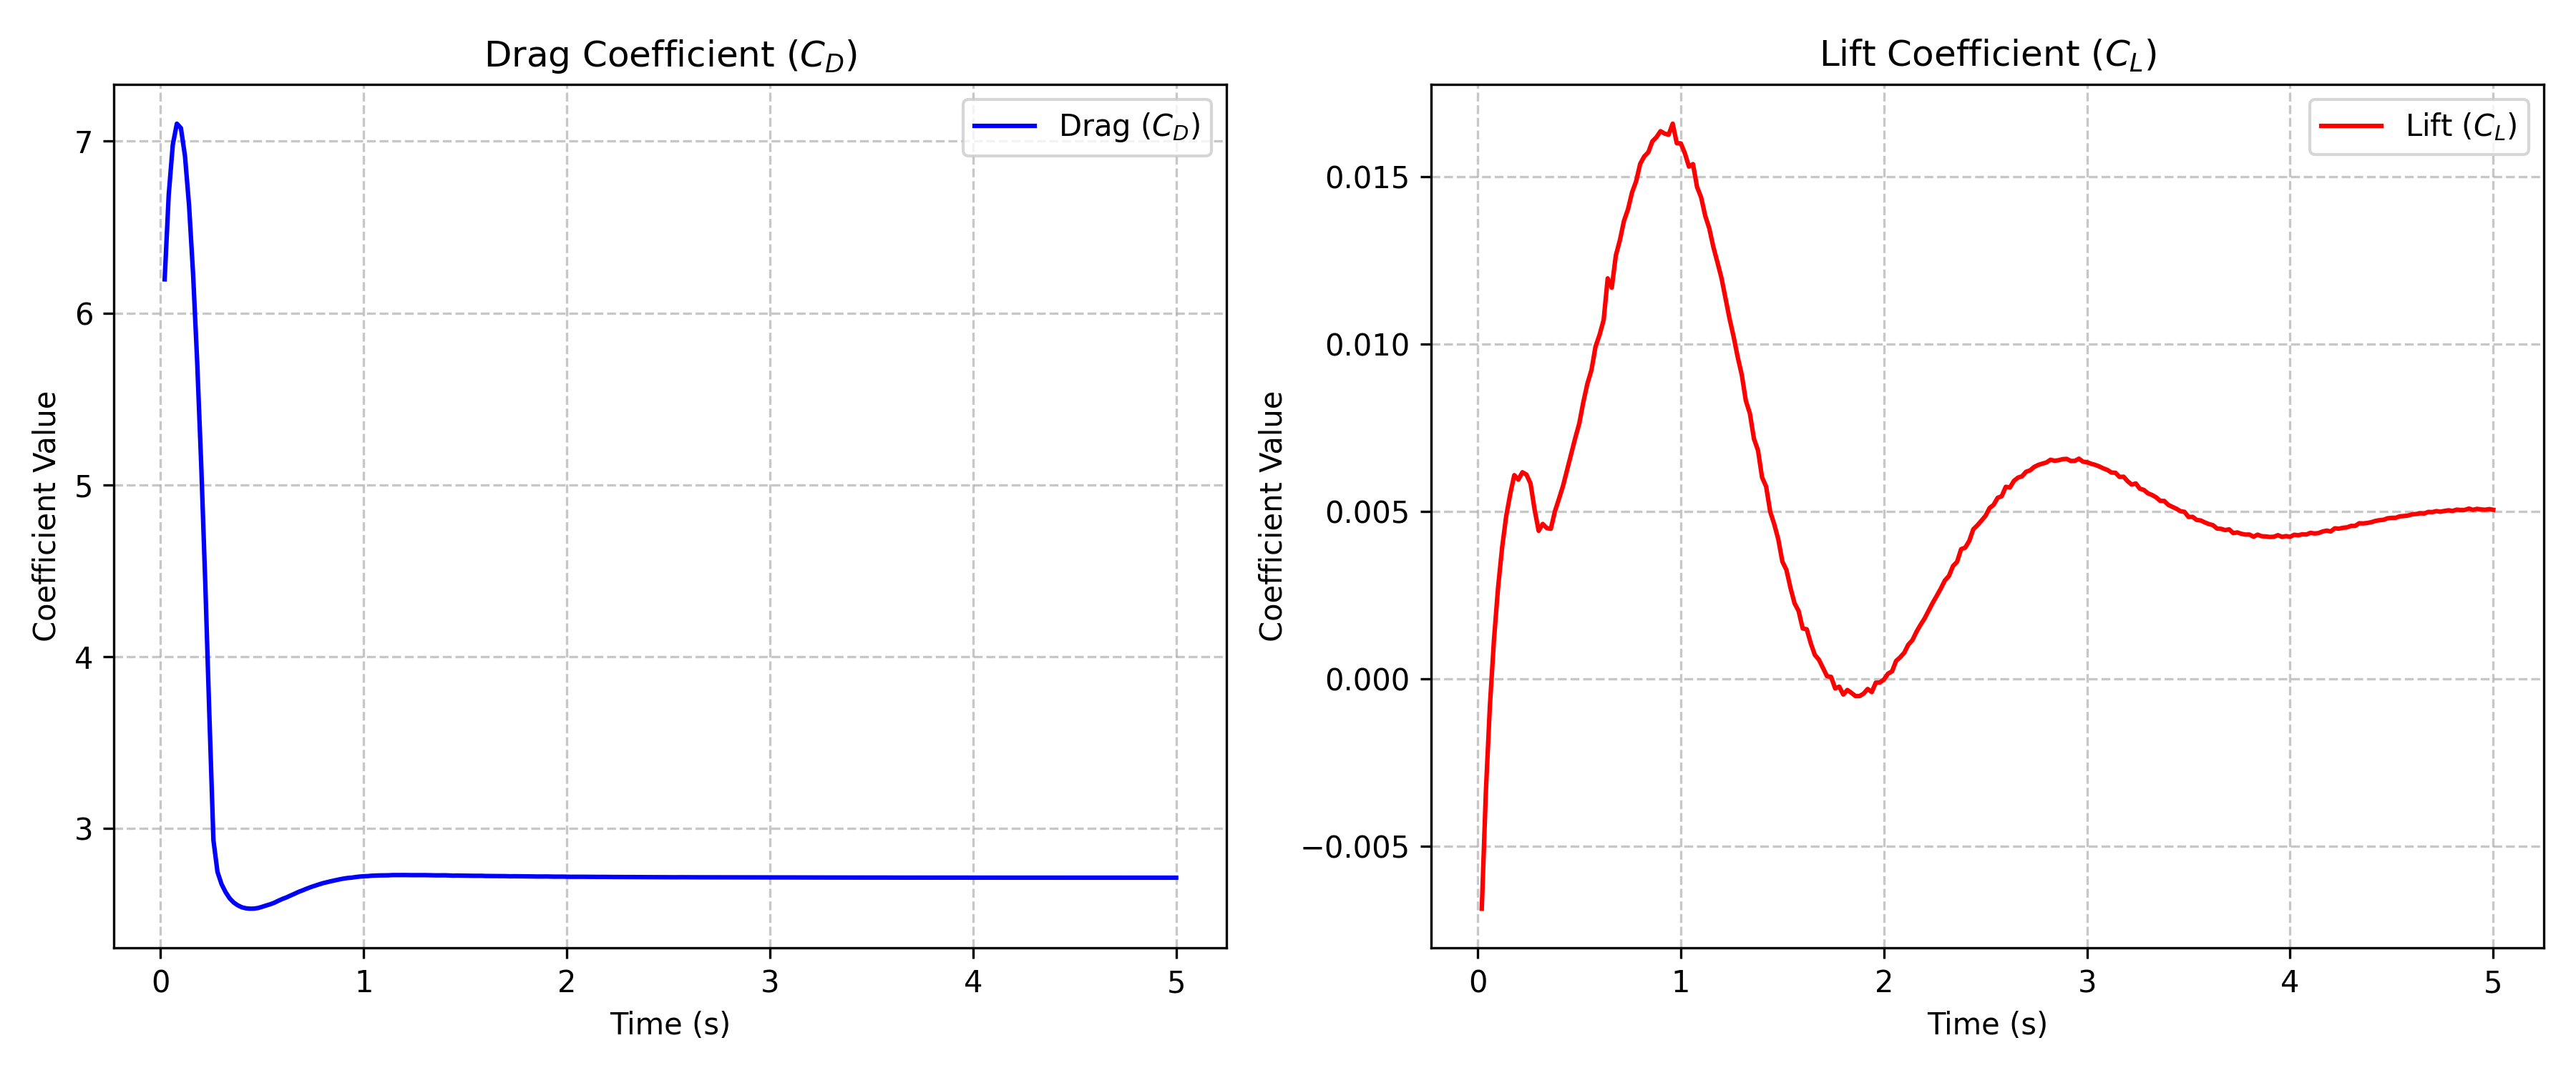
\includegraphics[width=1\textwidth]{Images/Test_cases/2D/Test_1/coefficients_plot_coarse_2D_CASE1.png}%
    }
    \hfill 
    \subfloat[Fine mesh. \label{fig:2d_1_fine_dl}]{%
        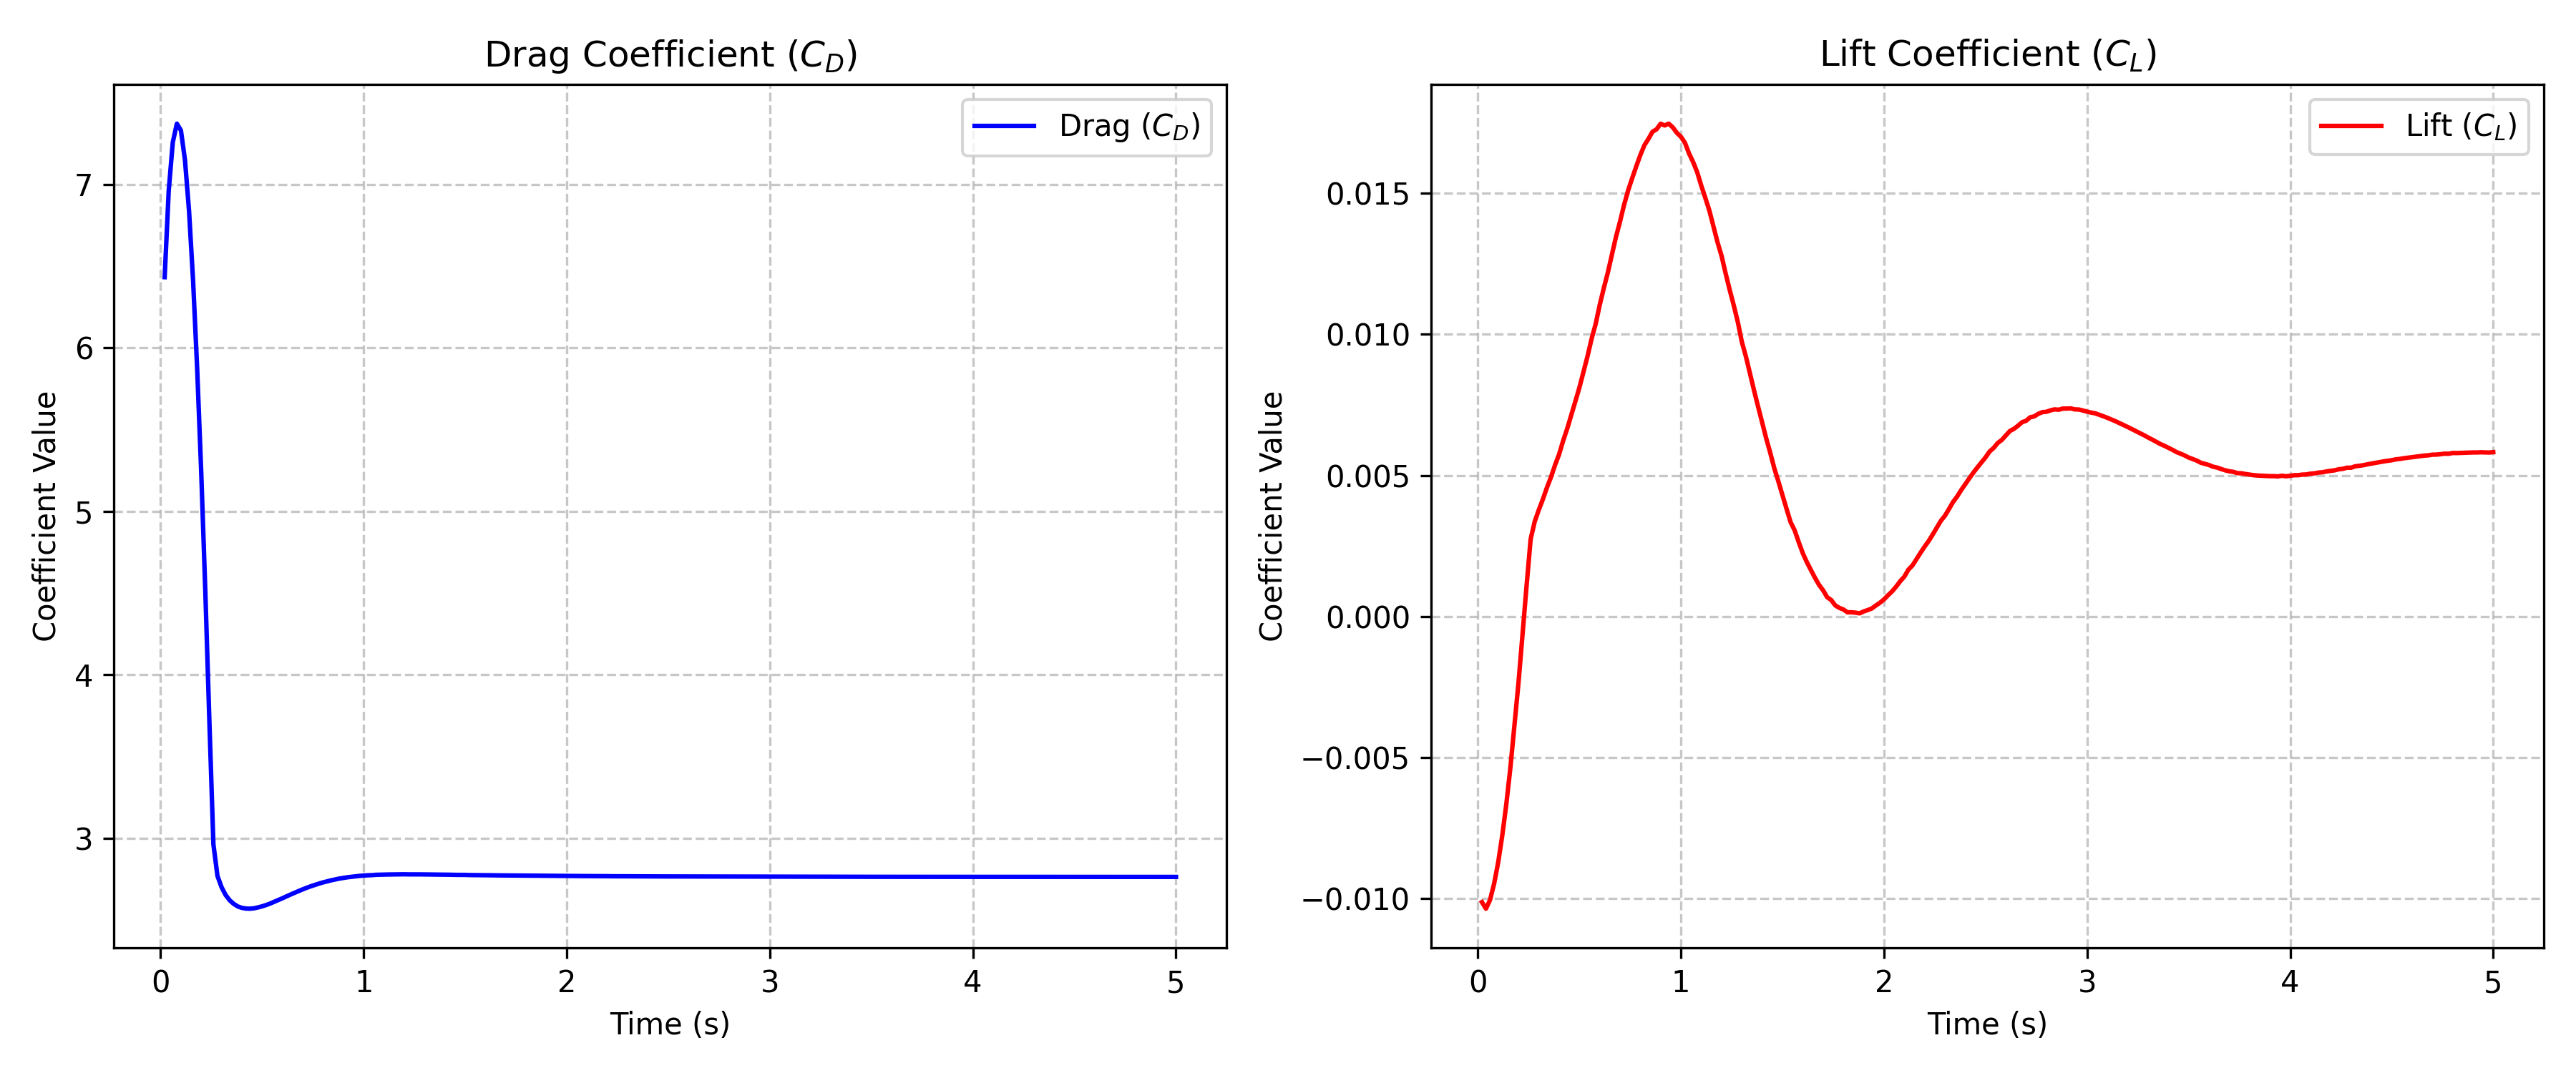
\includegraphics[width=1\textwidth]{Images/Test_cases/2D/Test_1/coefficients_plot_fine_2D_CASE1.png}%
    }
    \caption{Drag and lift coefficients for the 2D-1 steady test case.}
    \label{fig:2d_1_dl}
\end{figure}

%-----------------------------------------------
% 2D TEST CASE 2
%-----------------------------------------------
\begin{figure}[p]
    \centering
    \subfloat[Coarse mesh. \label{fig:2d_2_coarse_dl}]{%
        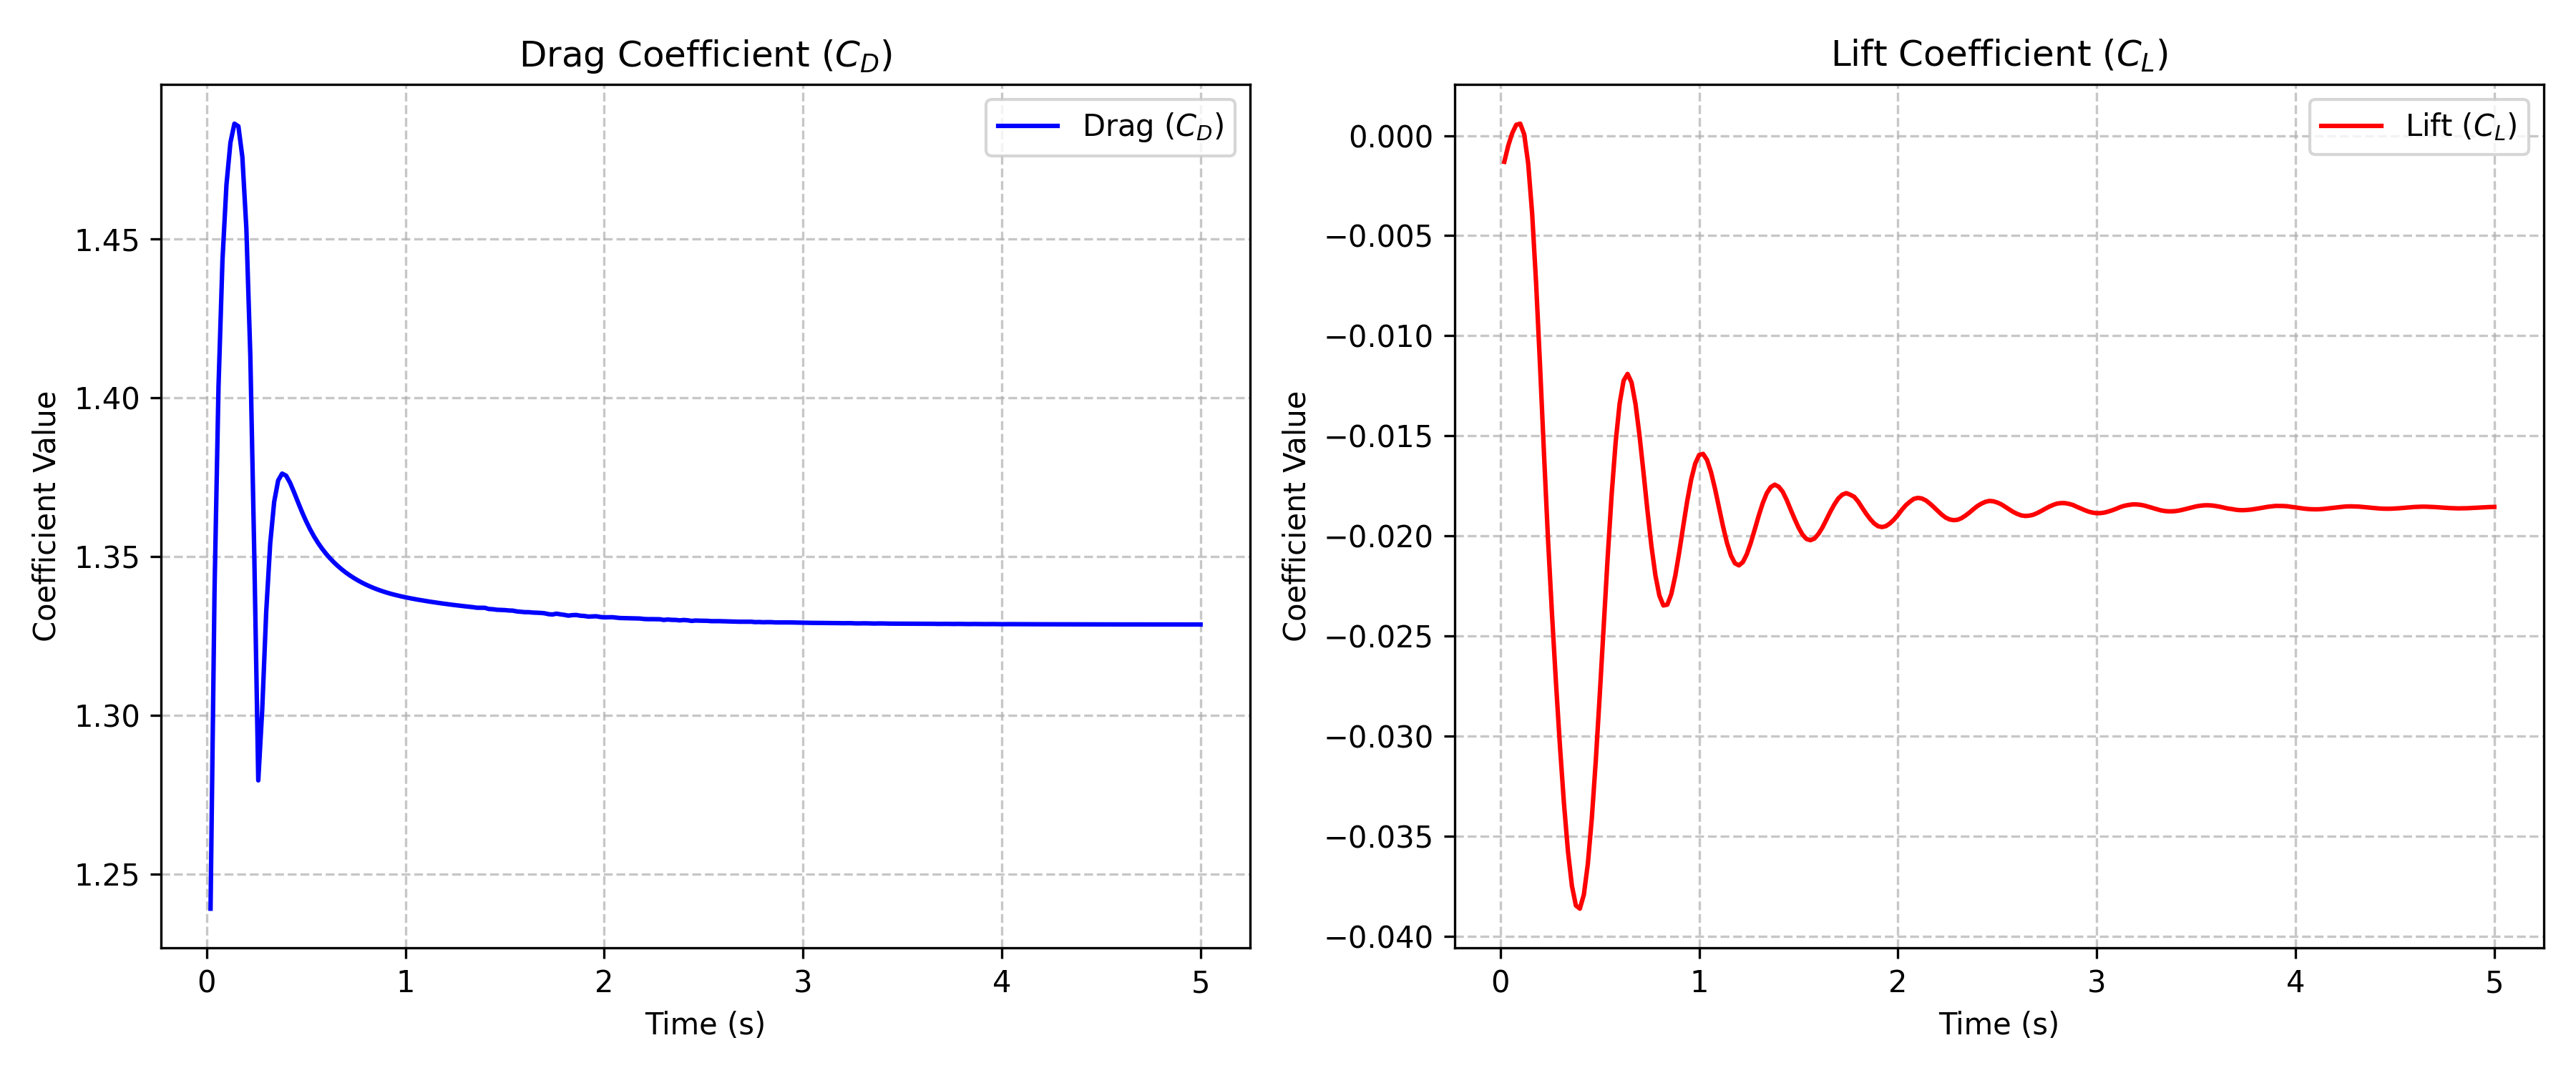
\includegraphics[width=1\textwidth]{Images/Test_cases/2D/Test_2/coefficients_plot_coarse_2D_CASE2.png}%
    }
    \hfill 
    \subfloat[Fine mesh. \label{fig:2d_2_fine_dl}]{%
        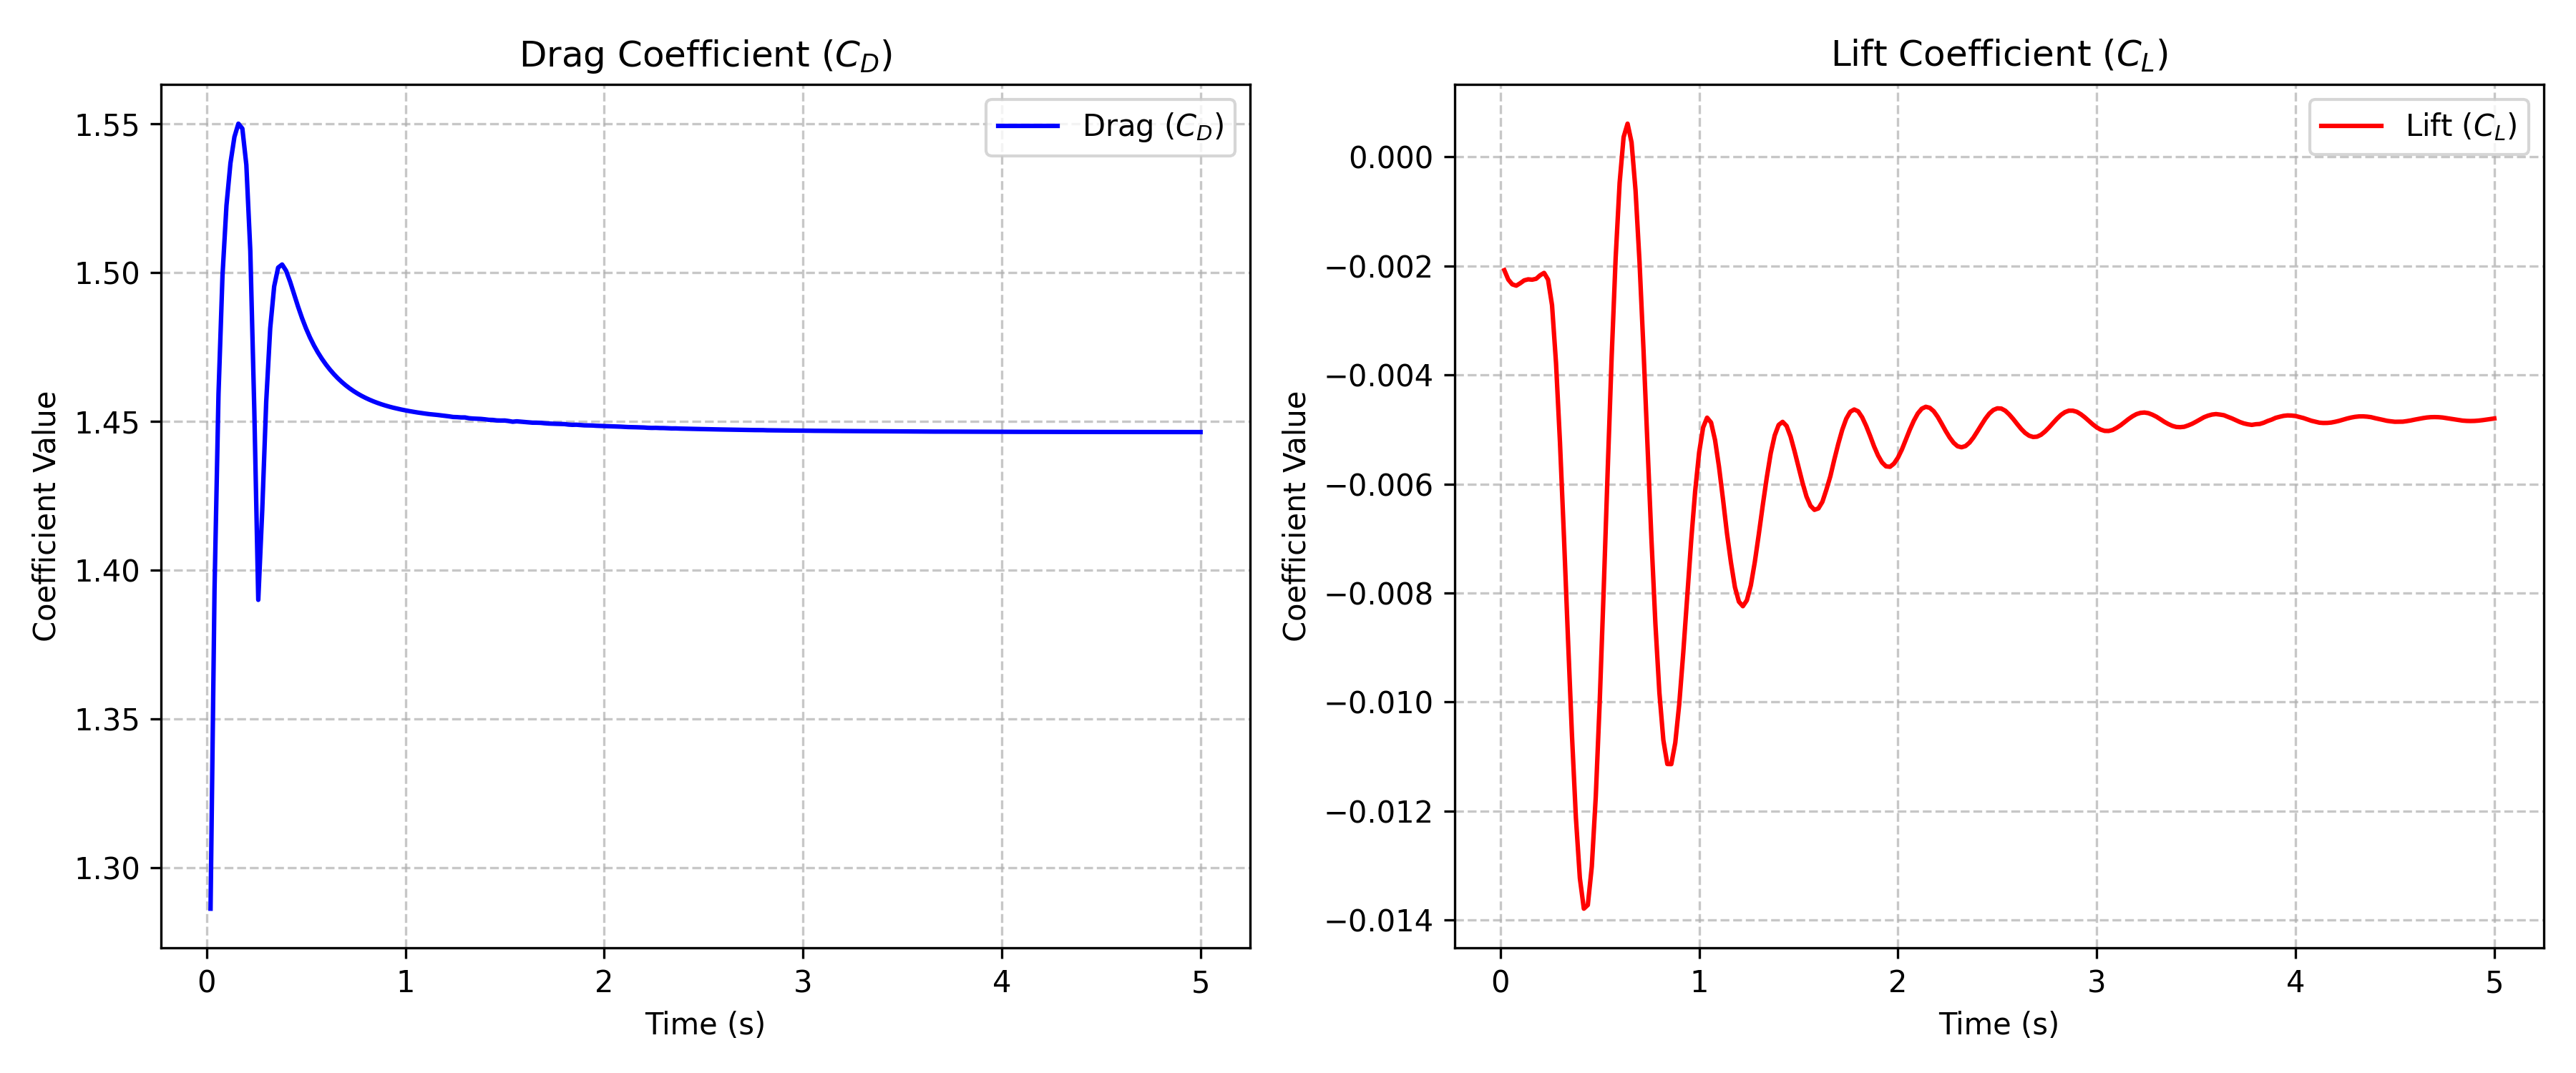
\includegraphics[width=1\textwidth]{Images/Test_cases/2D/Test_2/coefficients_plot_fine_2D_CASE2.png}%
    }
    \caption{Drag and lift coefficients for the 2D-2 steady test case.}
    \label{fig:2d_2_dl}
\end{figure}

%-----------------------------------------------
% 2D TEST CASE 3
%-----------------------------------------------
\begin{figure}[p]
    \centering
    \subfloat[Coarse mesh. \label{fig:2d_3_coarse_dl}]{%
        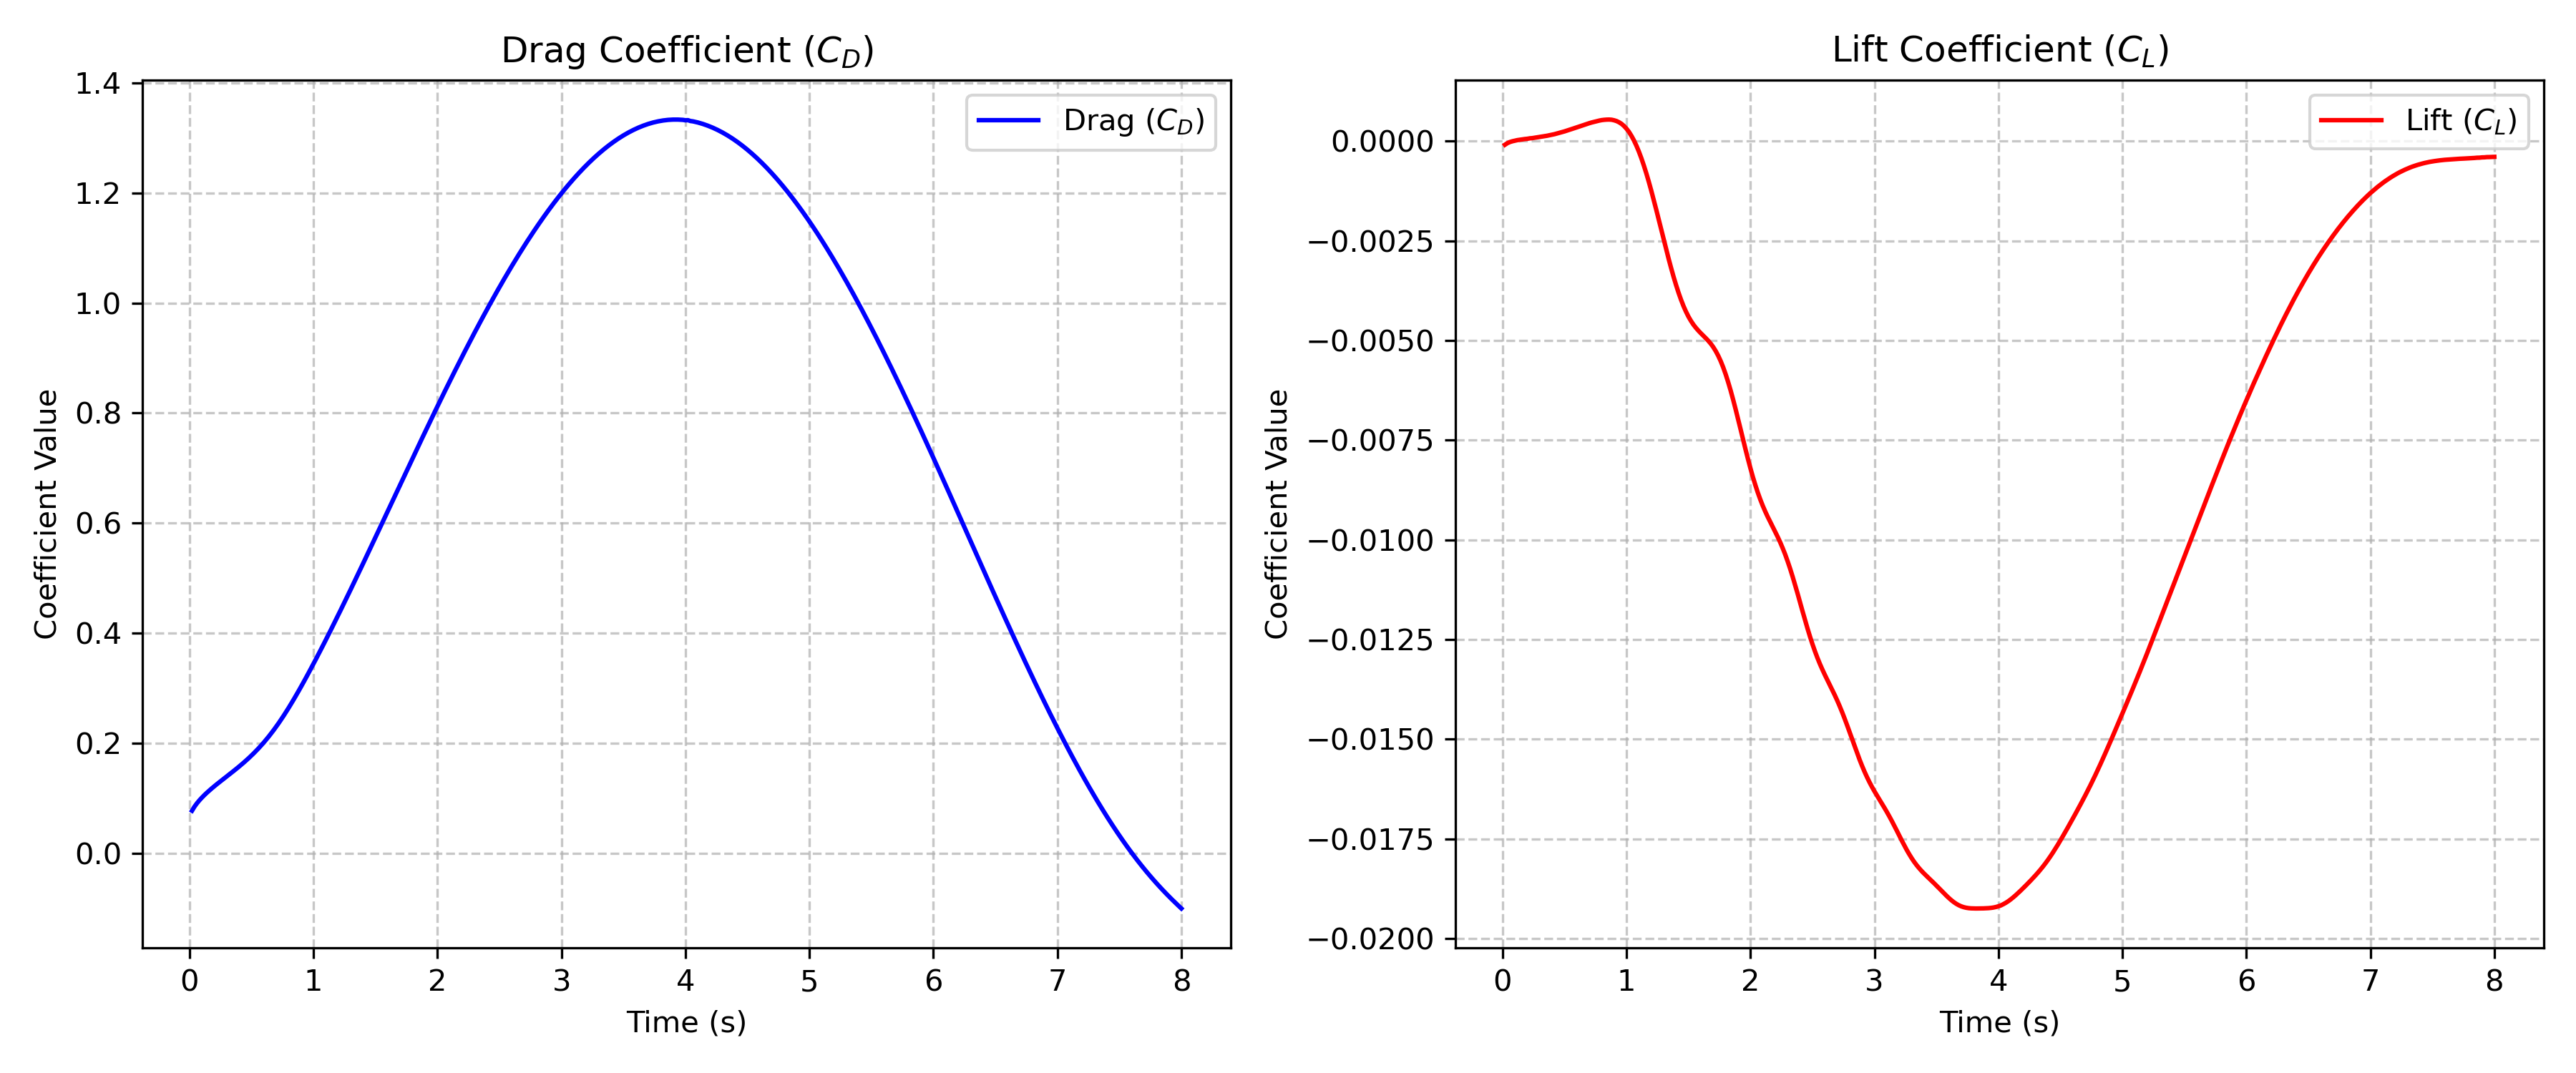
\includegraphics[width=1\textwidth]{Images/Test_cases/2D/Test_3/coefficients_plot_coarse.png}%
    }
    \hfill
    \subfloat[Fine mesh. \label{fig:2d_3_fine_dl}]{%
        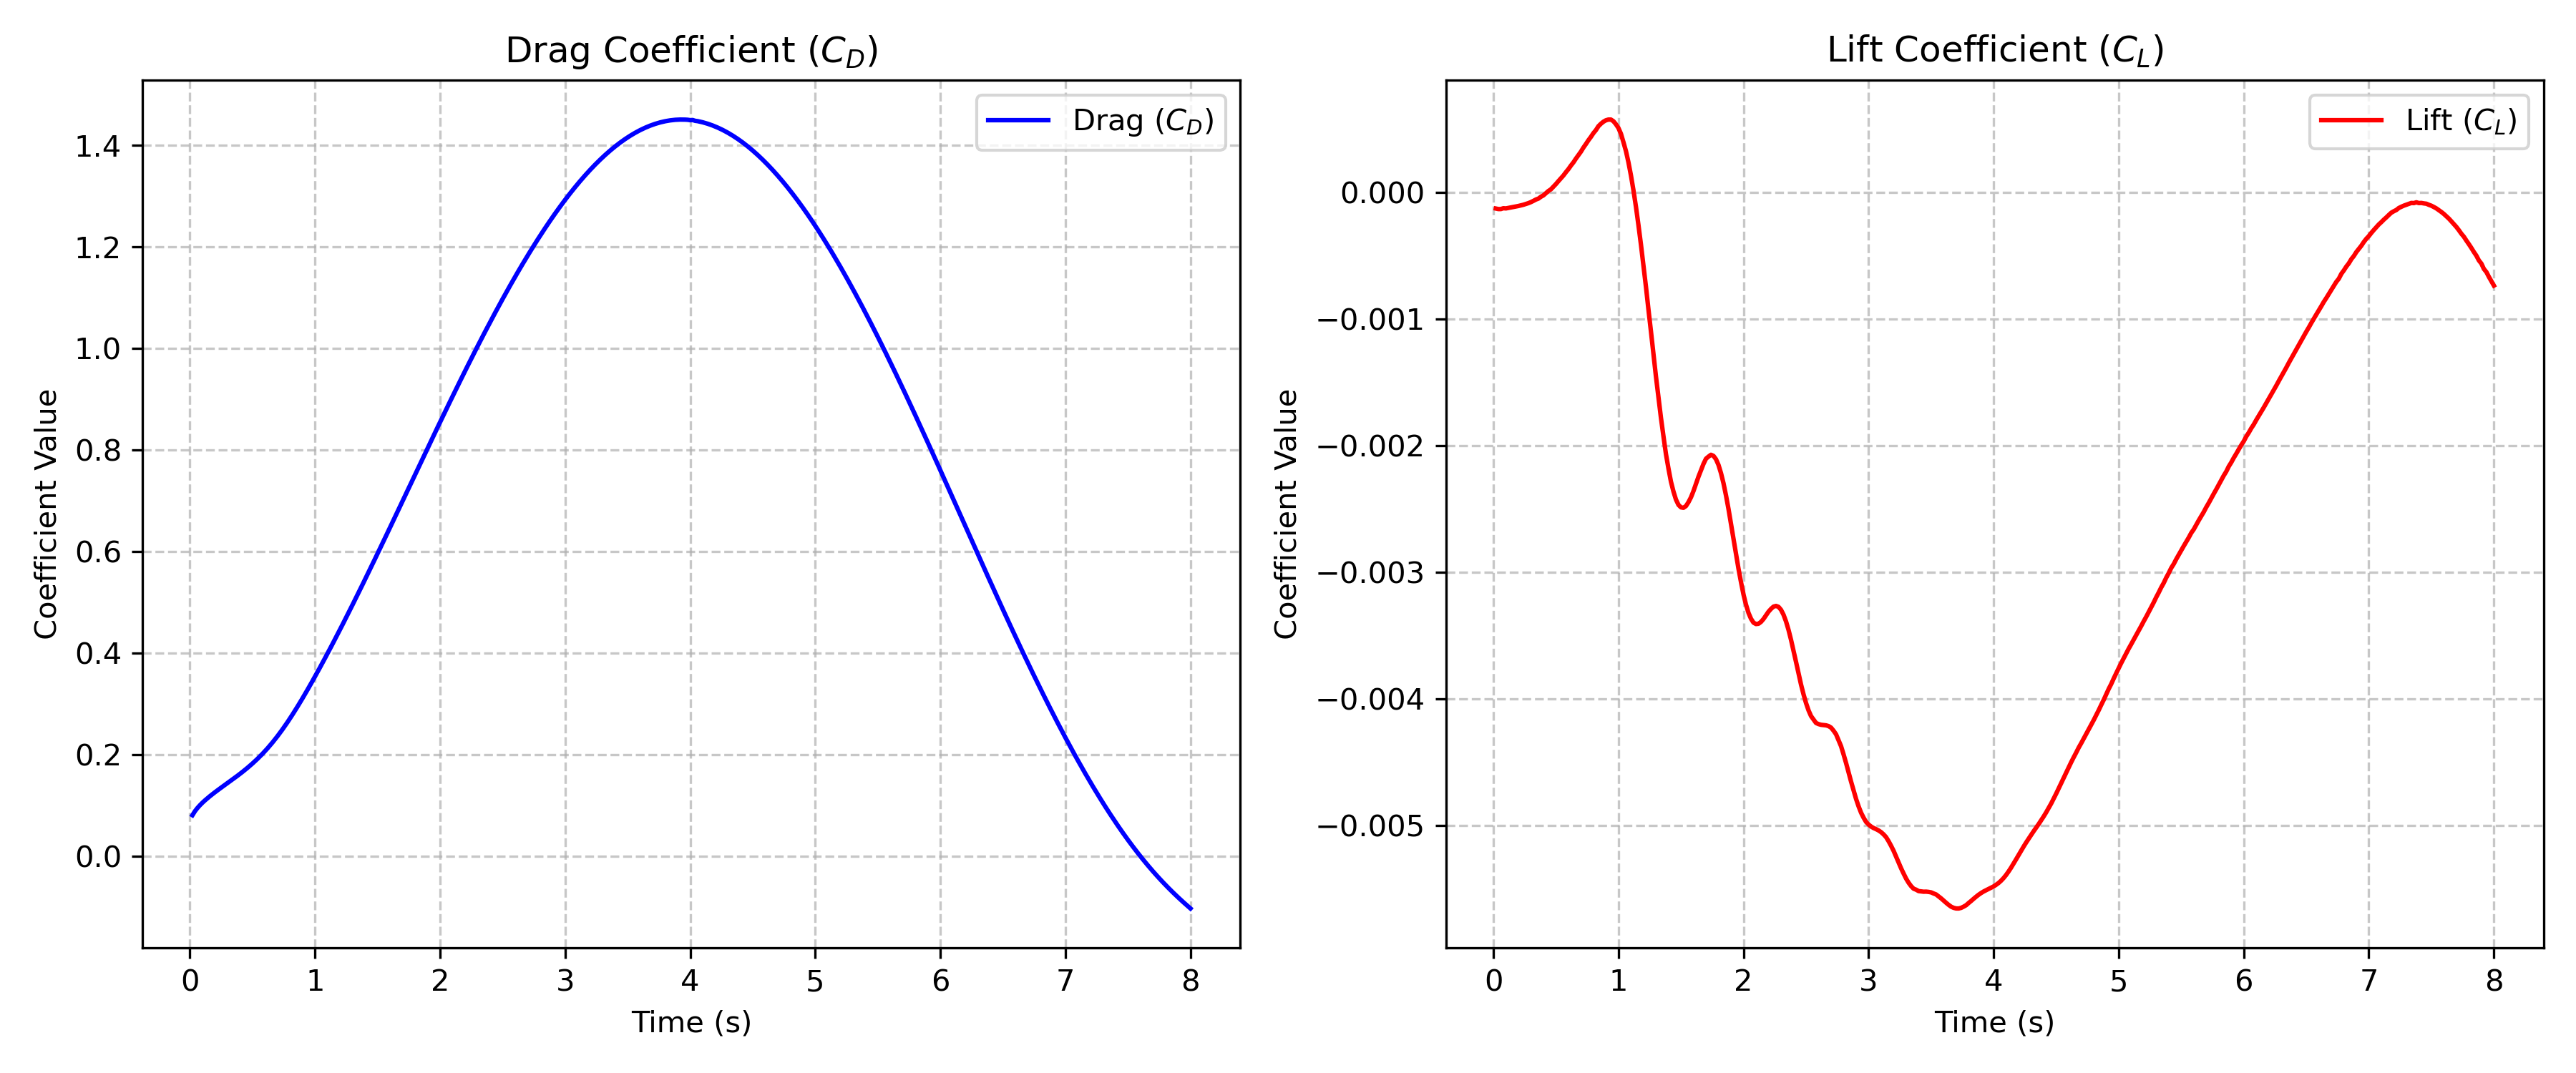
\includegraphics[width=1\textwidth]{Images/Test_cases/2D/Test_3/coefficients_plot_fine.png}%
    }
    \caption{Drag and lift coefficients for the 2D-3 unsteady test case.}
    \label{fig:2d_3_dl}
\end{figure}

%-----------------------------------------------
% 3D TEST CASE 1
%-----------------------------------------------
\begin{figure}[p]
    \centering
    % Cylinder Comparison
    \subfloat[Cylinder: Coarse mesh \label{fig:3d_1_cylinder_coarse_dl}]{
        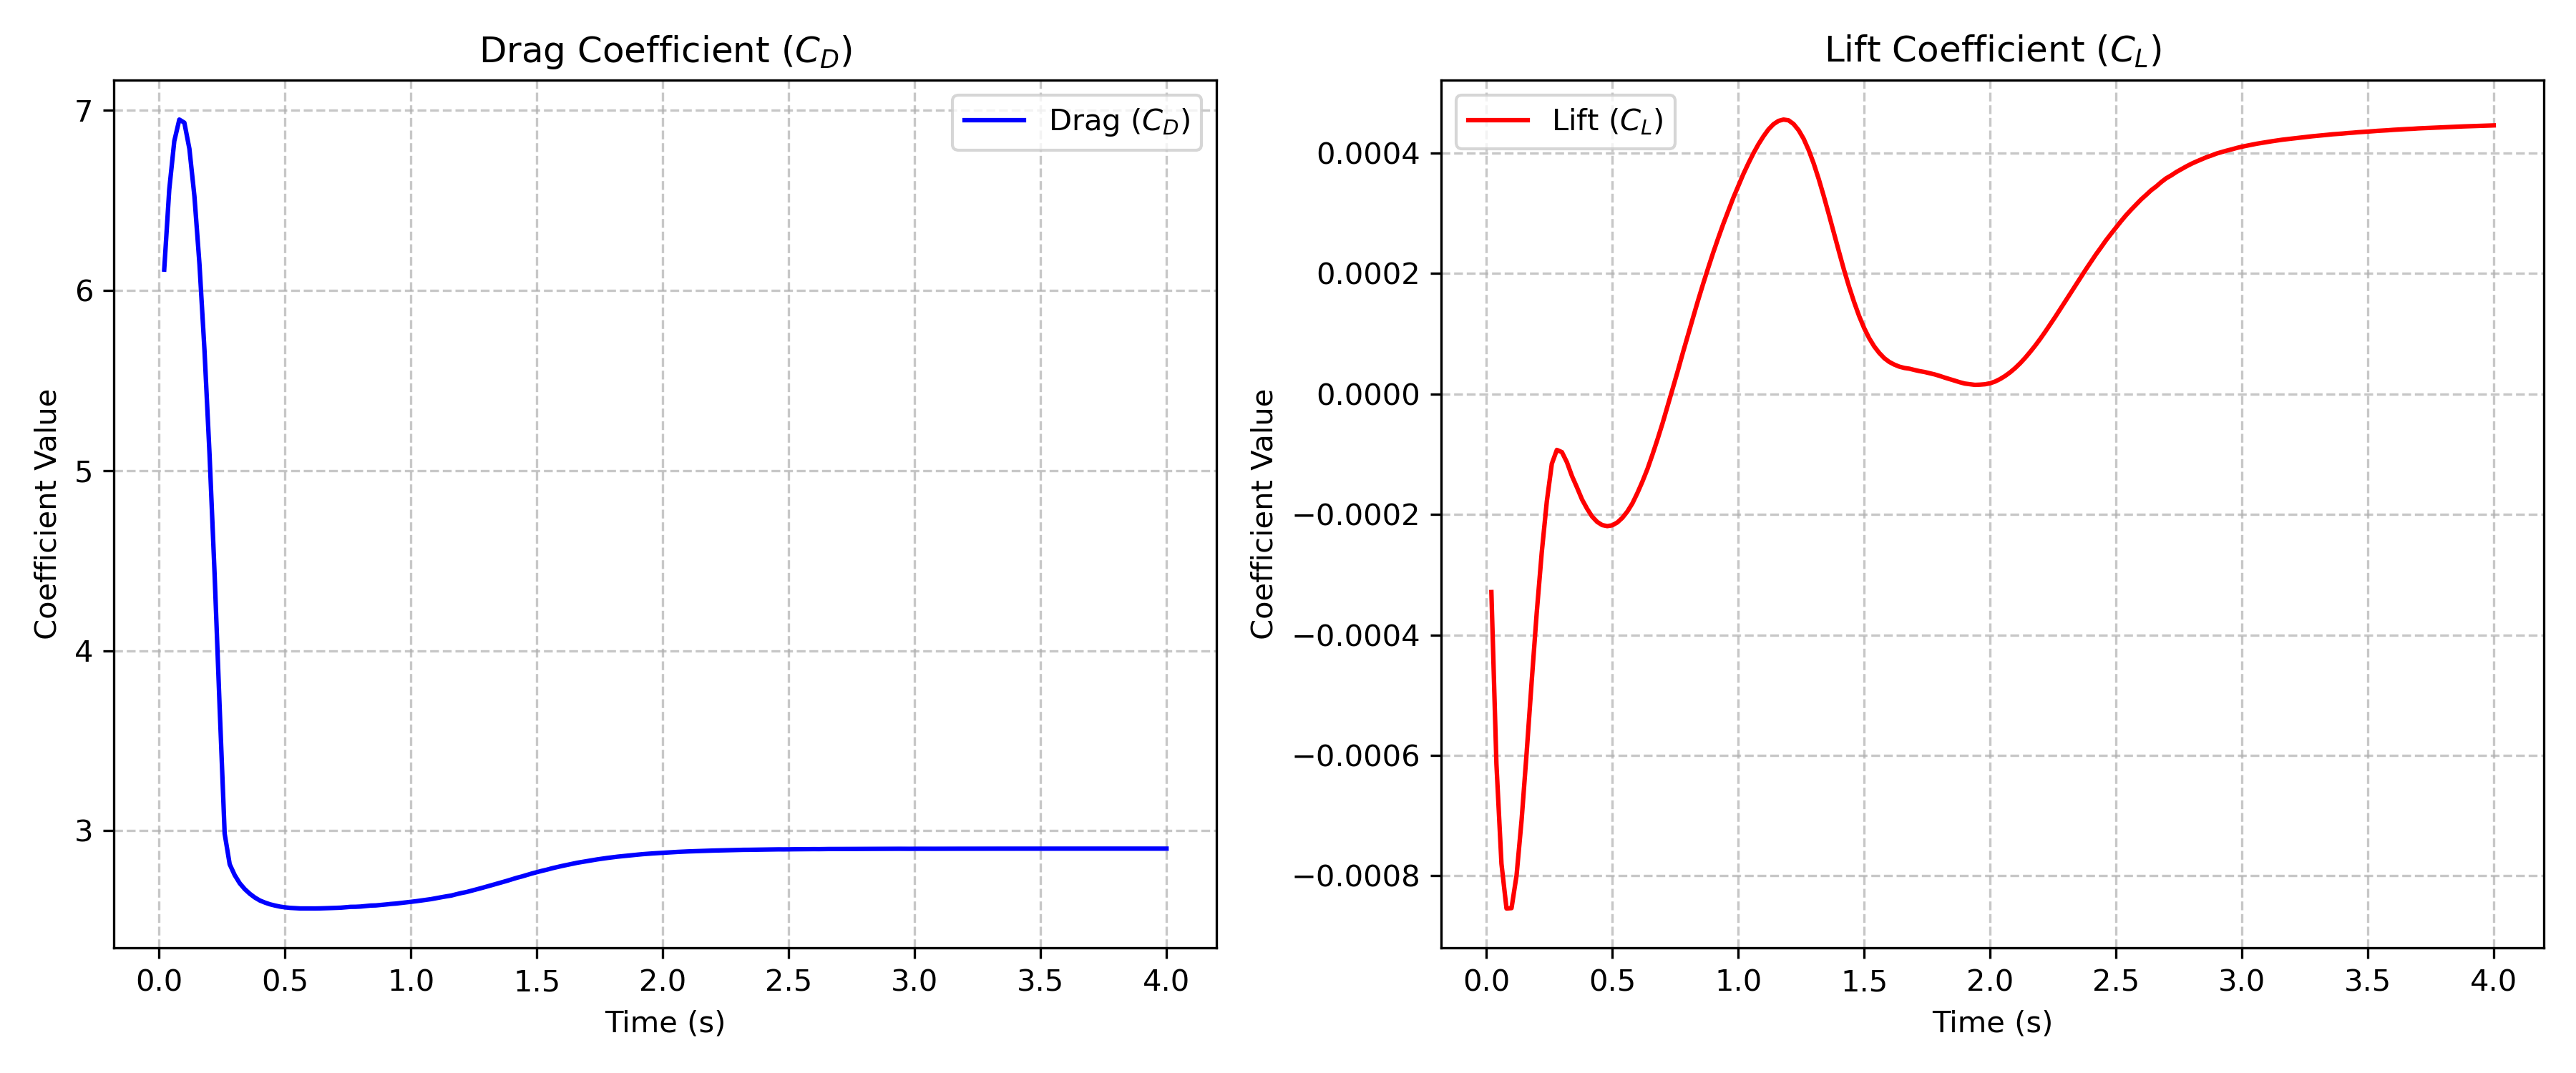
\includegraphics[width=0.75\textwidth]{coefficients_plot_cylinder_coarse.png}
    }
    \\
    \subfloat[Cylinder: Fine mesh\label{fig:3d_1_cylinder_fine_dl}]{
        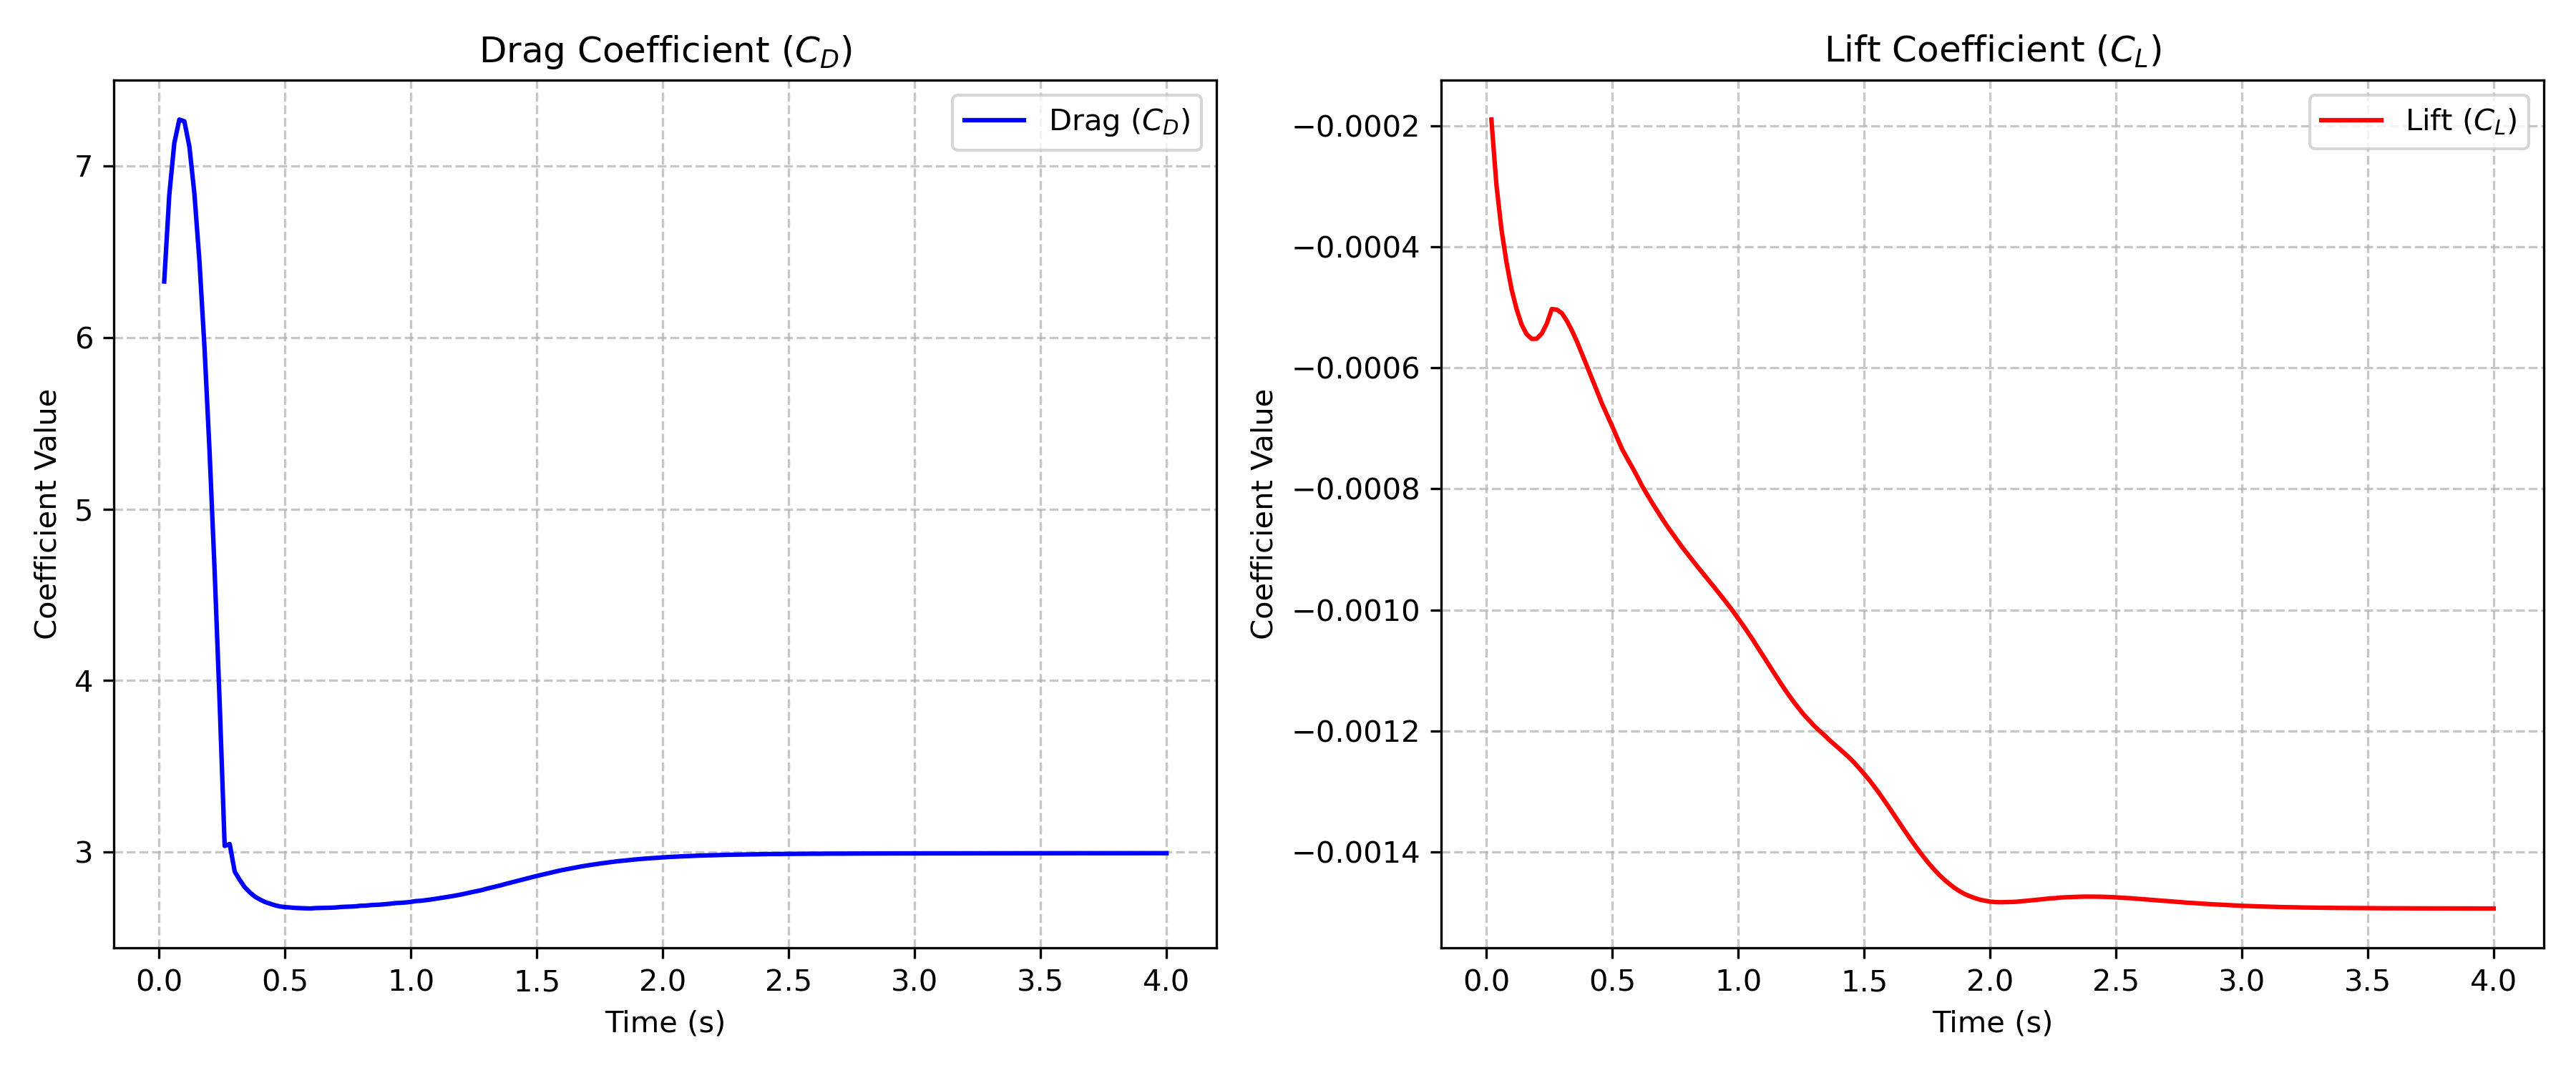
\includegraphics[width=0.75\textwidth]{coefficients_plot_cylinder_fine.png}
    }
    \\ \vspace{1em}
    % Parallelepiped Comparison
    \subfloat[Parallelepiped: Coarse mesh \label{fig:3d_1_parallelepiped_coarse_dl}]{
        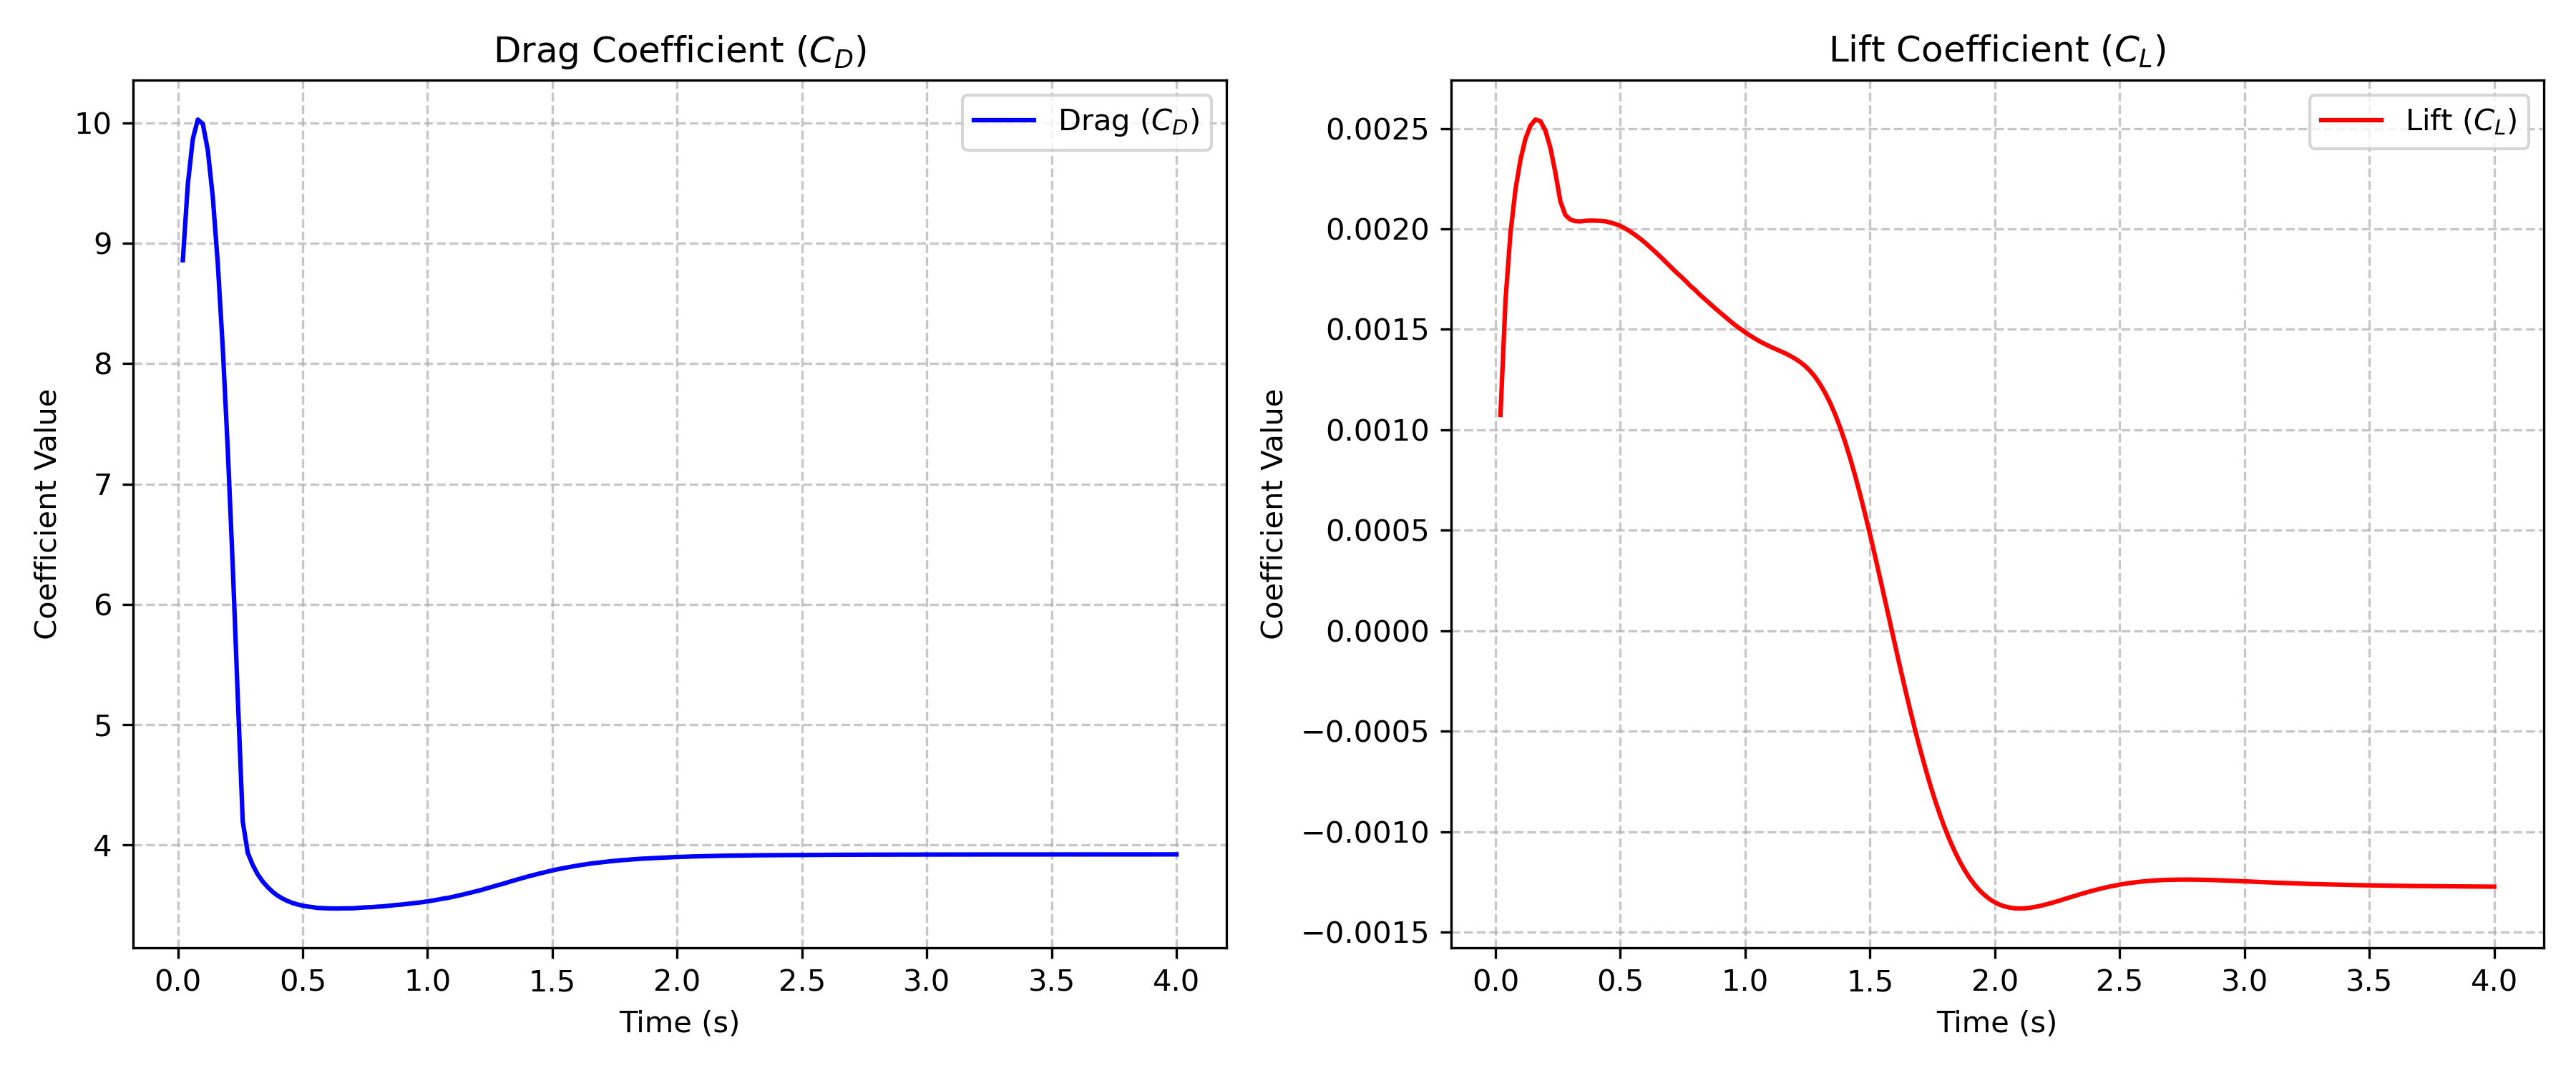
\includegraphics[width=0.75\textwidth]{coefficients_plot_parallelepiped_coarse.png}
    }
    \\
    \subfloat[Parallelepiped: Fine mesh \label{fig:3d_1_parallelepiped_fine_dl}]{
        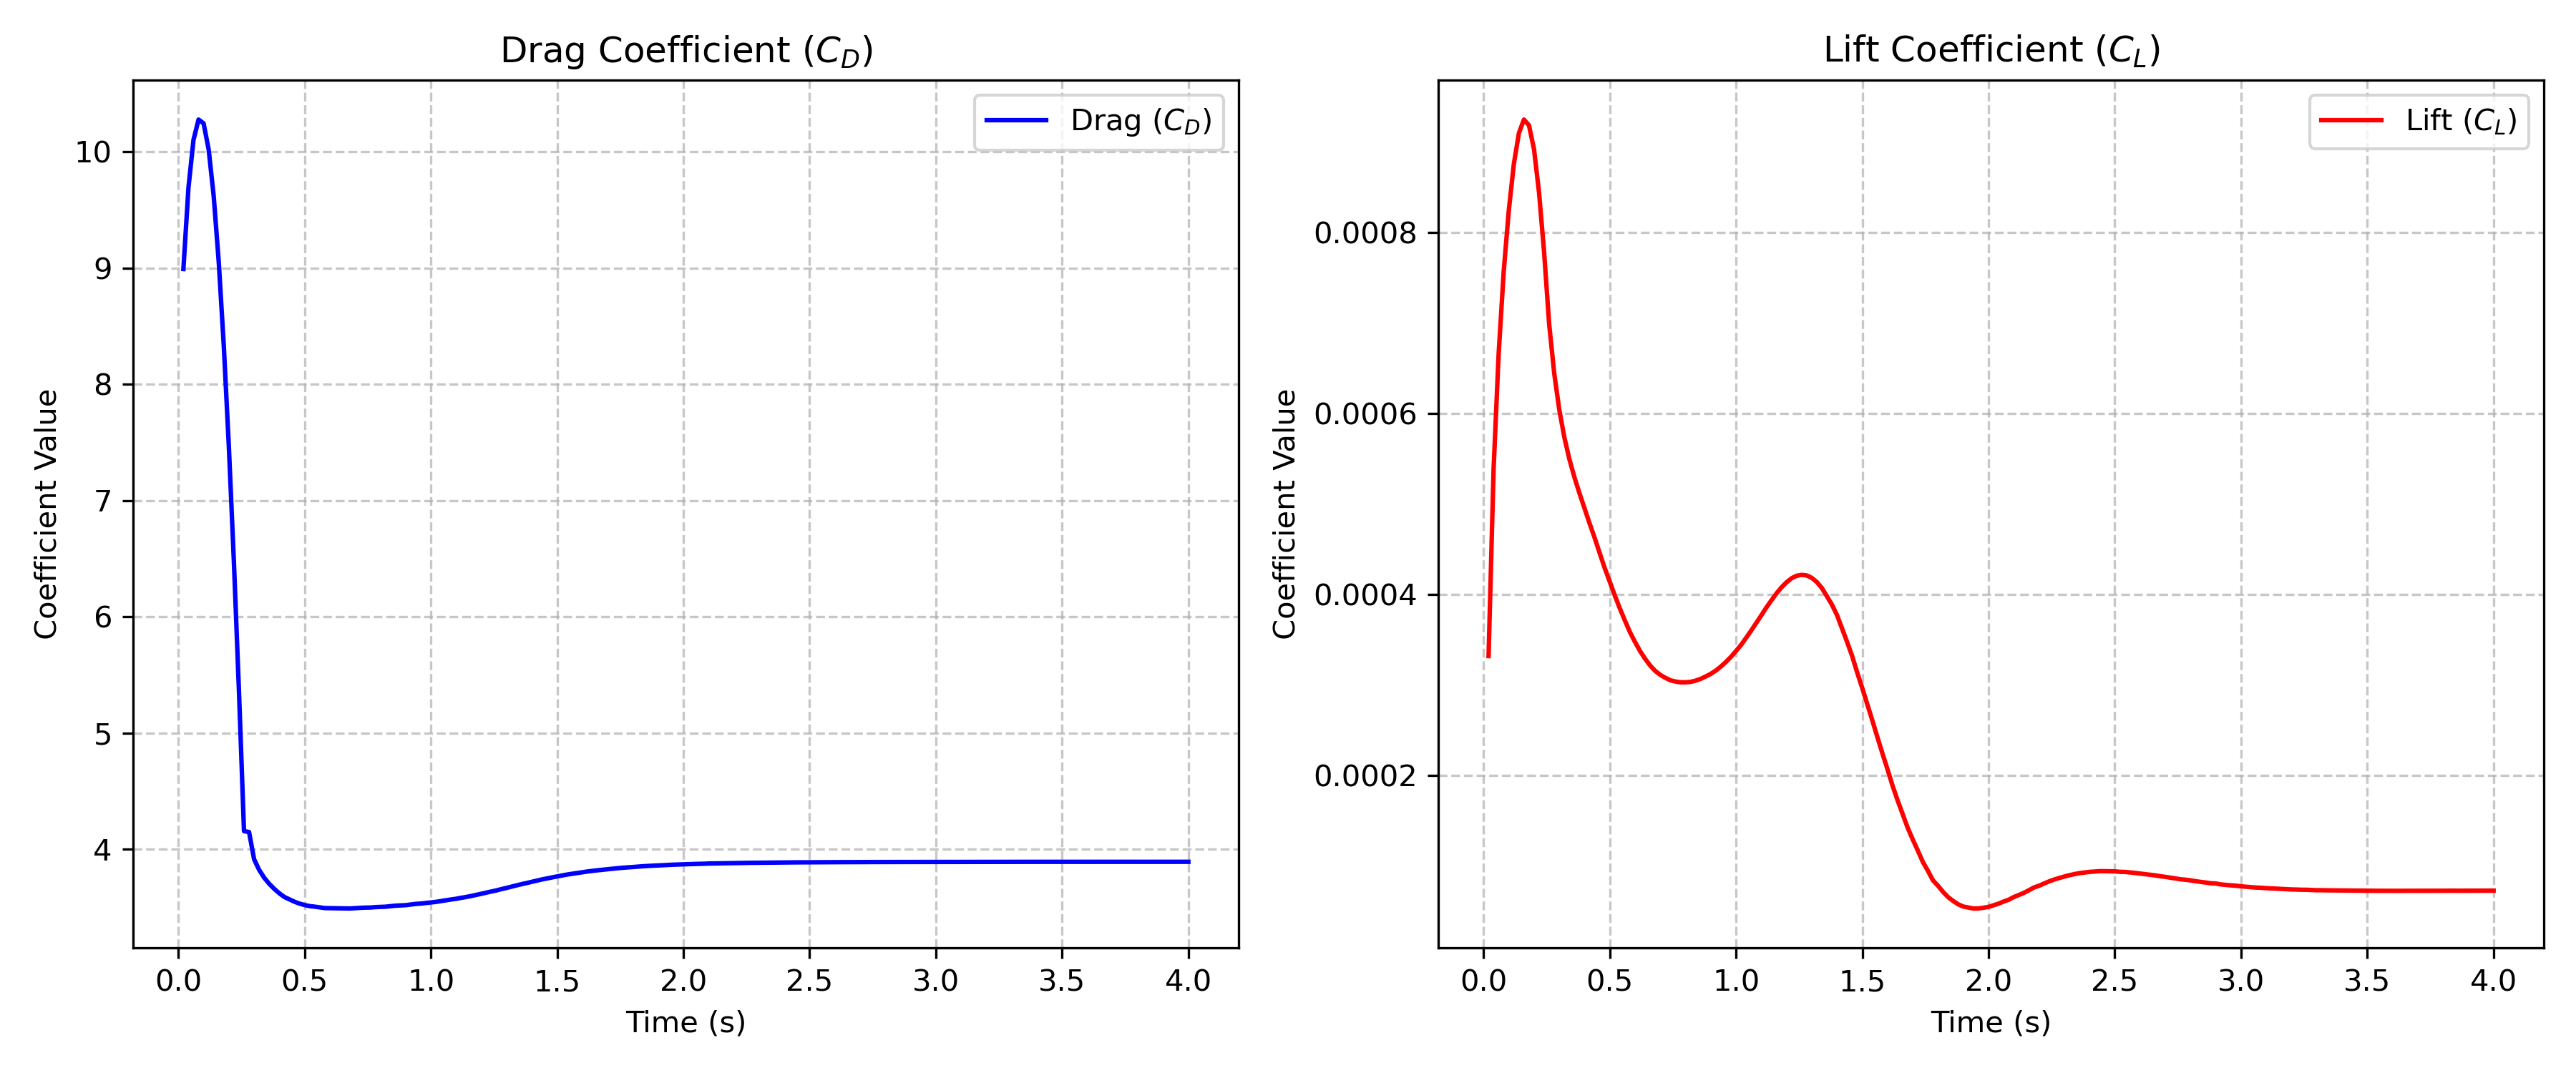
\includegraphics[width=0.75\textwidth]{coefficients_plot_parallelepiped_fine.png}
    }
    \caption{Drag and Lift coefficients (Cylinder and Parallelepiped) for the 3D-1 steady test case.}
    \label{fig:3d_1_dl}
\end{figure}

%-----------------------------------------------
% 3D TEST CASE 2
%-----------------------------------------------
\begin{figure}[p]
    \centering
    % Cylinder Comparison
    \subfloat[Cylinder: Coarse mesh \label{fig:3d_2_cylinder_coarse_dl}]{
        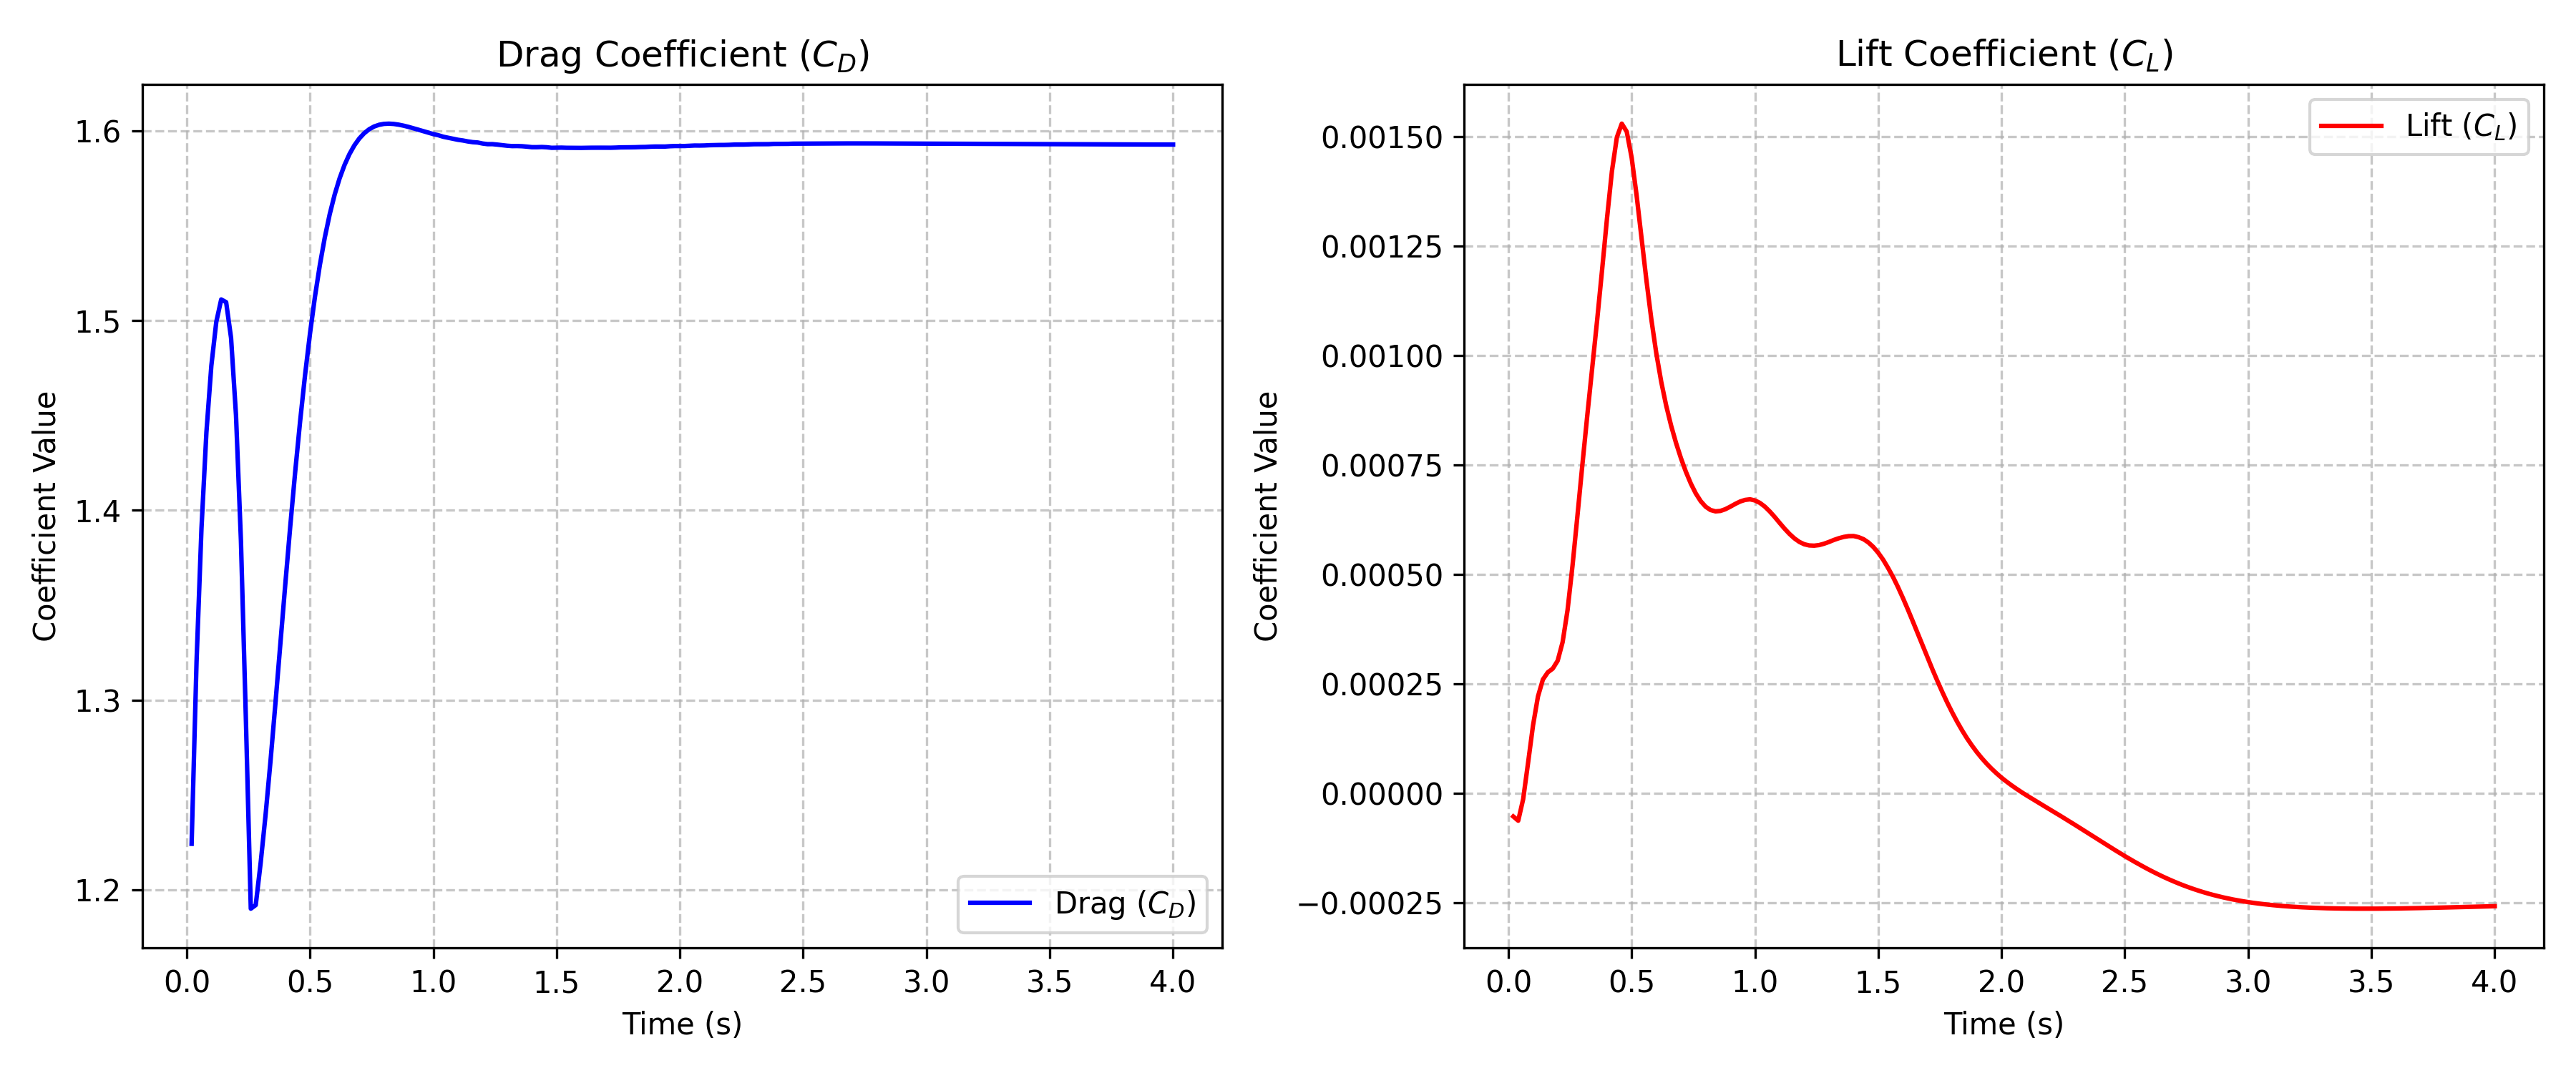
\includegraphics[width=0.75\textwidth]{cyl_coarse.png}
    }
    \\
    \subfloat[Cylinder: Fine mesh \label{fig:3d_2_cylinder_fine_dl}]{
        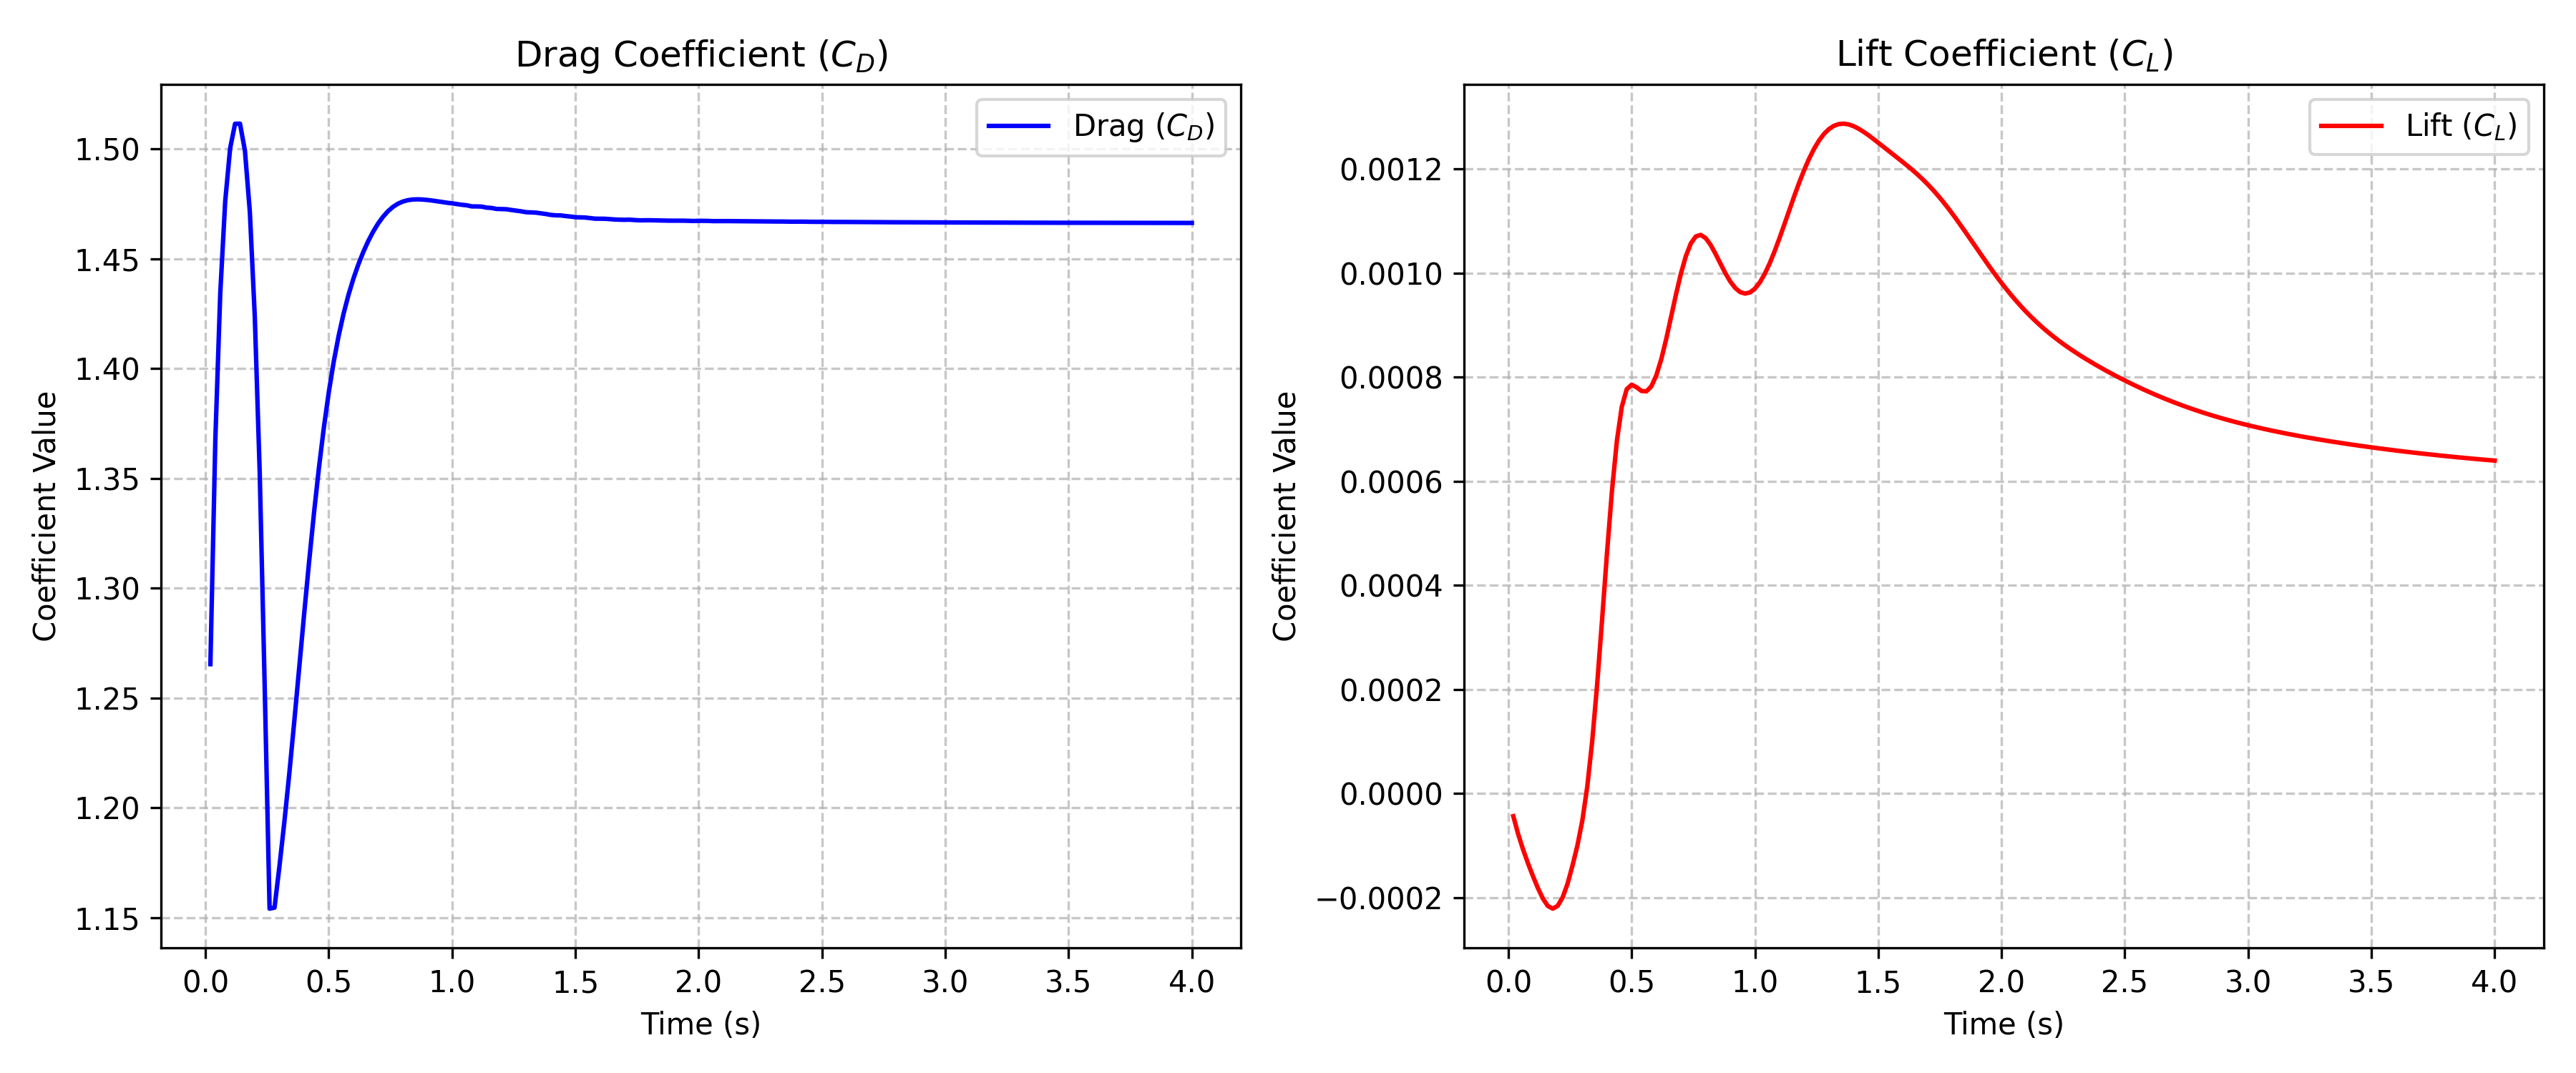
\includegraphics[width=0.75\textwidth]{drag_lift_test2.png}
    }
    \\ \vspace{1em}
    % Cylinder Comparison
    \subfloat[Parallelepiped: Coarse mesh \label{fig:3d_2_parallelepiped_coarse_dl}]{
        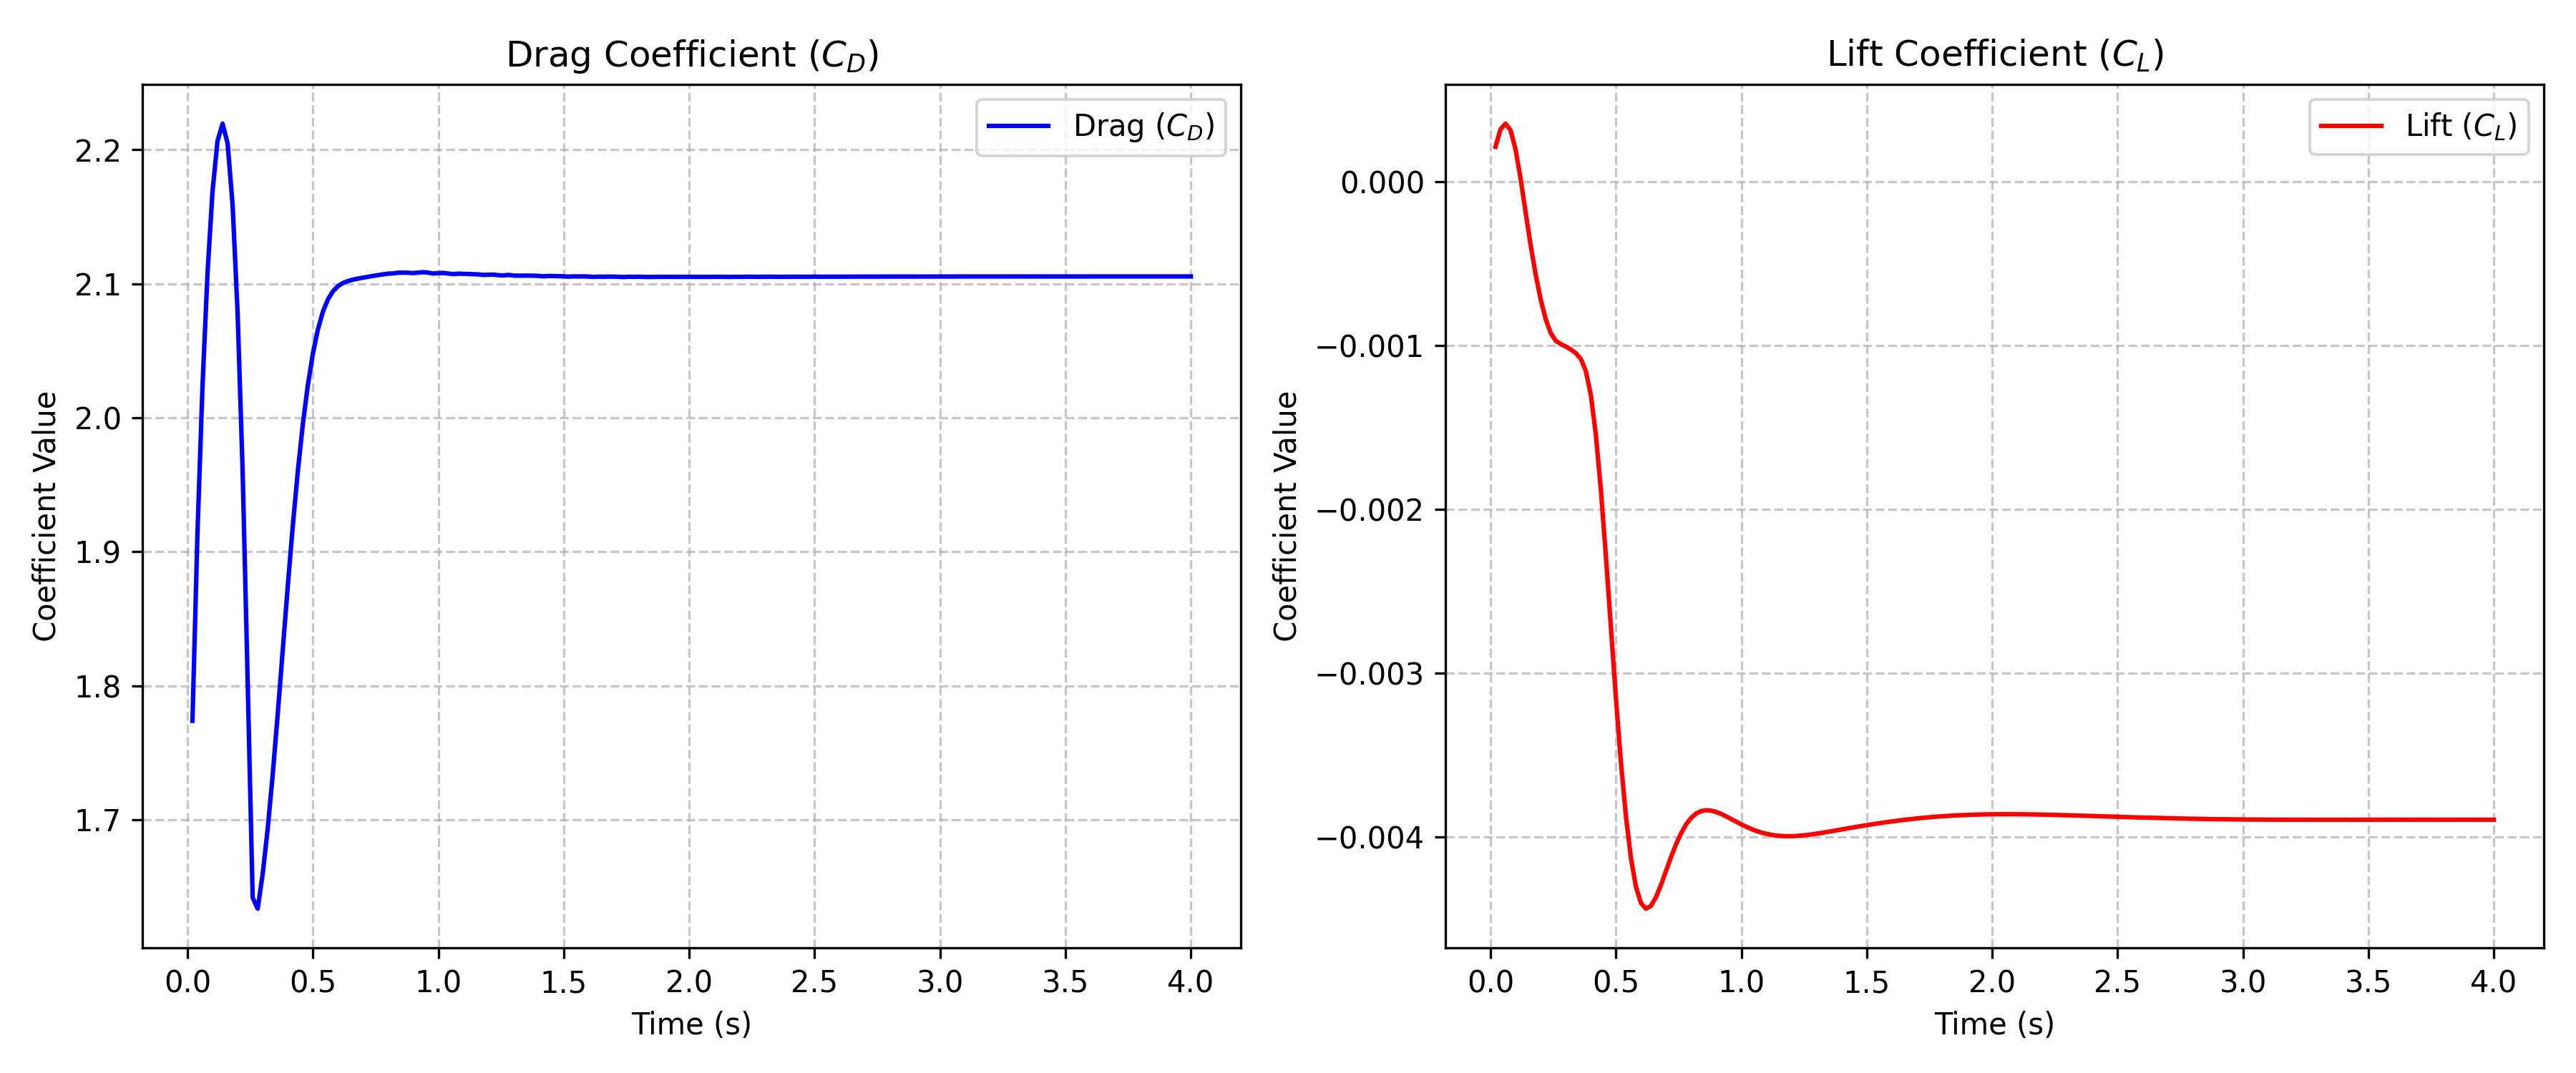
\includegraphics[width=0.75\textwidth]{drag_lift_coarse_test2.png}
    }
    \\ 
    \subfloat[Parallelepiped: Fine mesh \label{fig:3d_2_parallelepiped_fine_dl}]{
        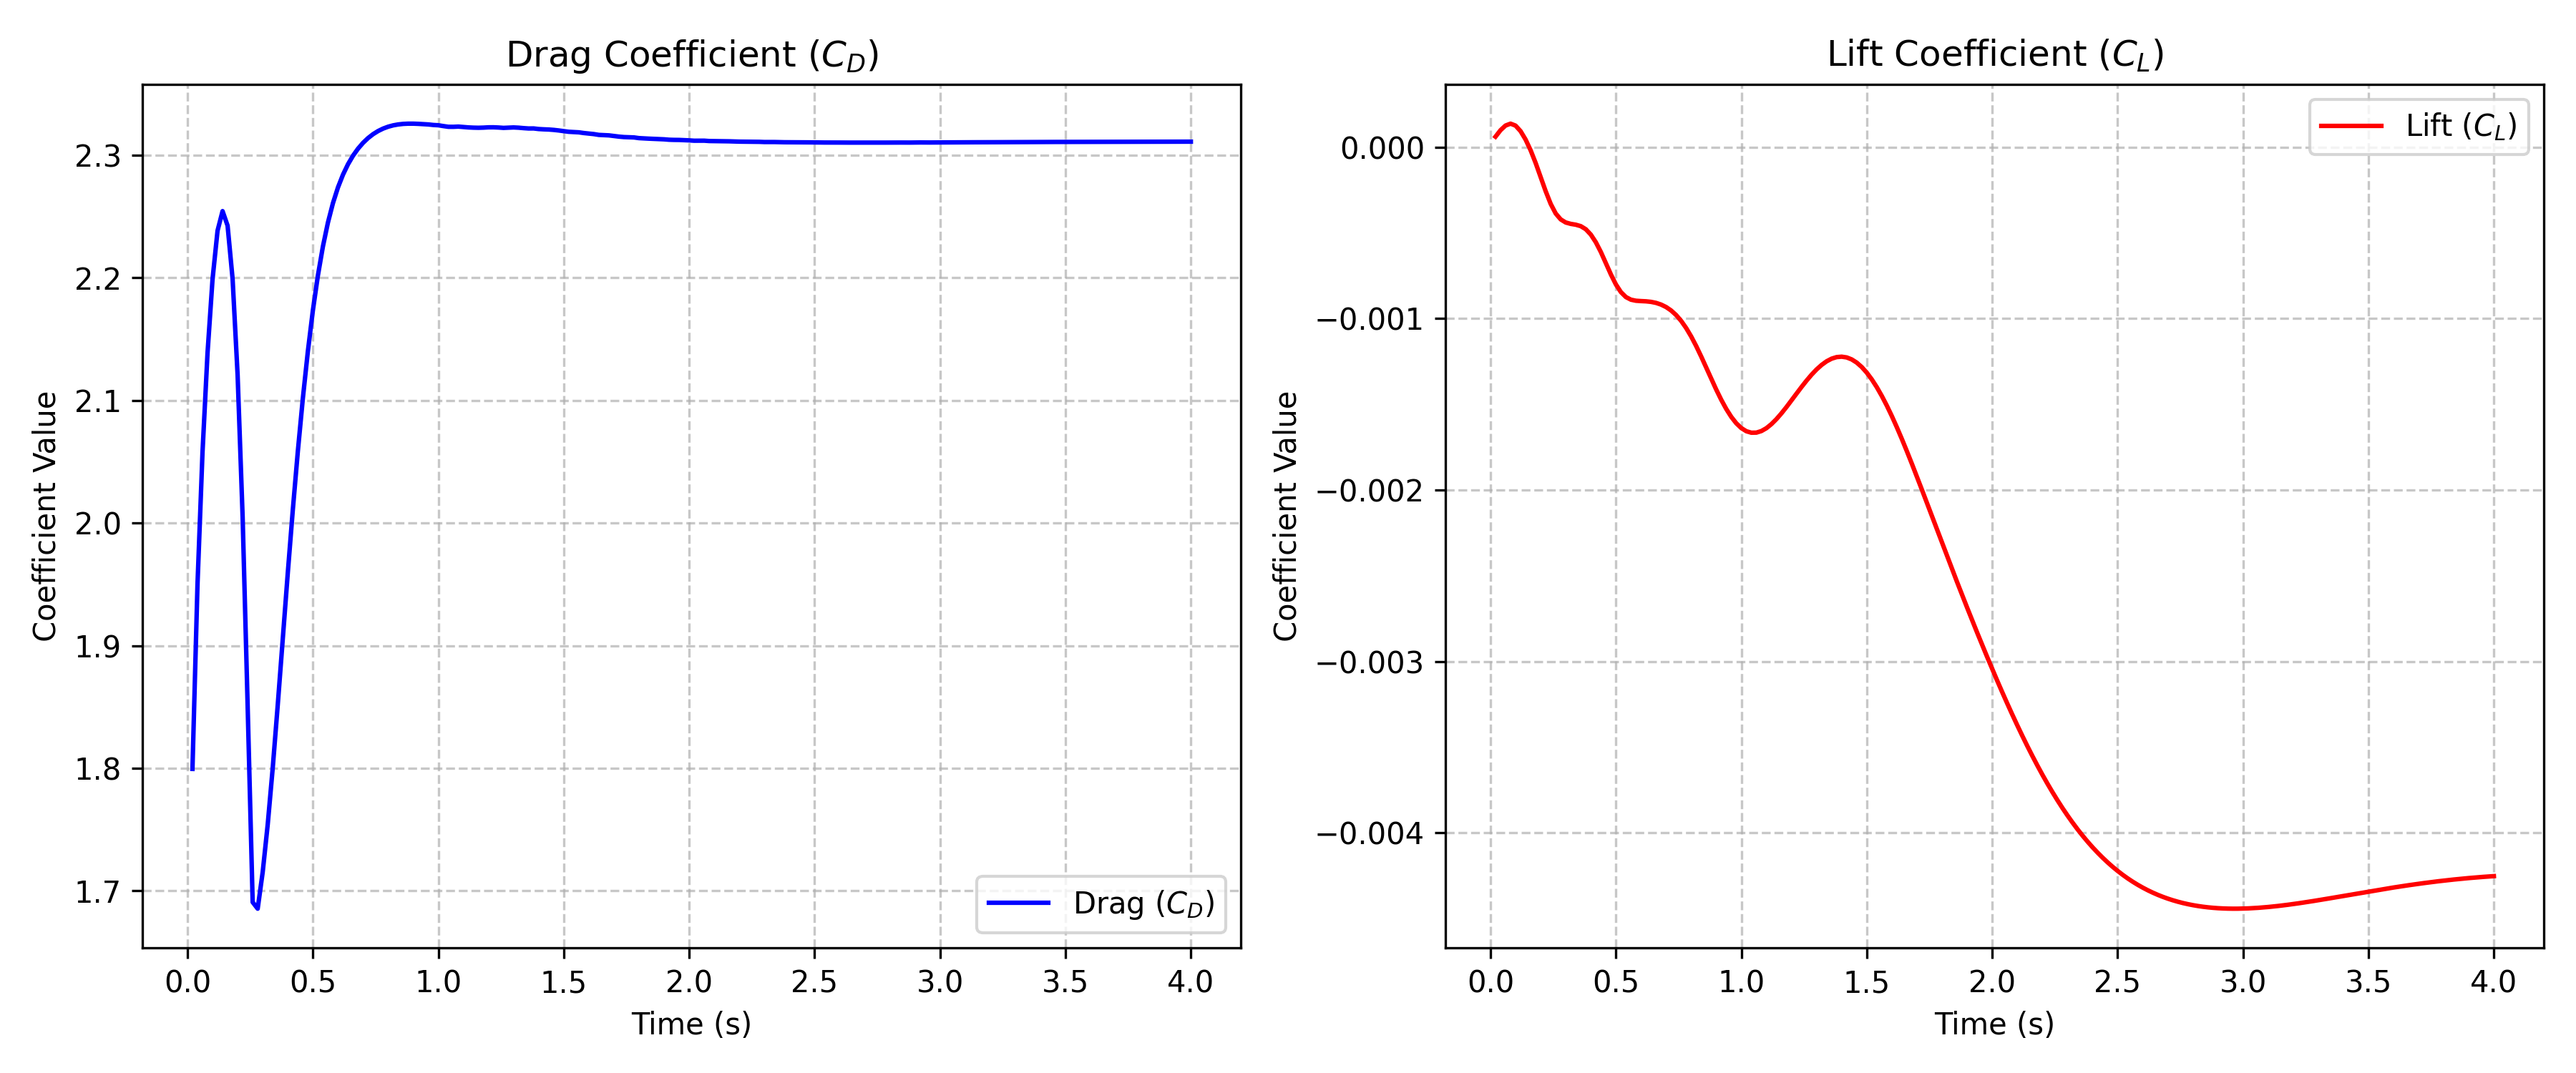
\includegraphics[width=0.75\textwidth]{drag_lift_fine_test2.png}
    }
    \caption{Drag and Lift coefficients (Cylinder and Parallelepiped) for the 3D-2 steady test case.}
    \label{fig:3d_2_dl}
\end{figure}

%-----------------------------------------------
% 3D TEST CASE 3
%-----------------------------------------------
\begin{figure}[p]
    \centering
    % Cylinder Comparison
    \subfloat[Cylinder: Coarse mesh \label{fig:3d_3_cylinder_coarse_dl}]{
        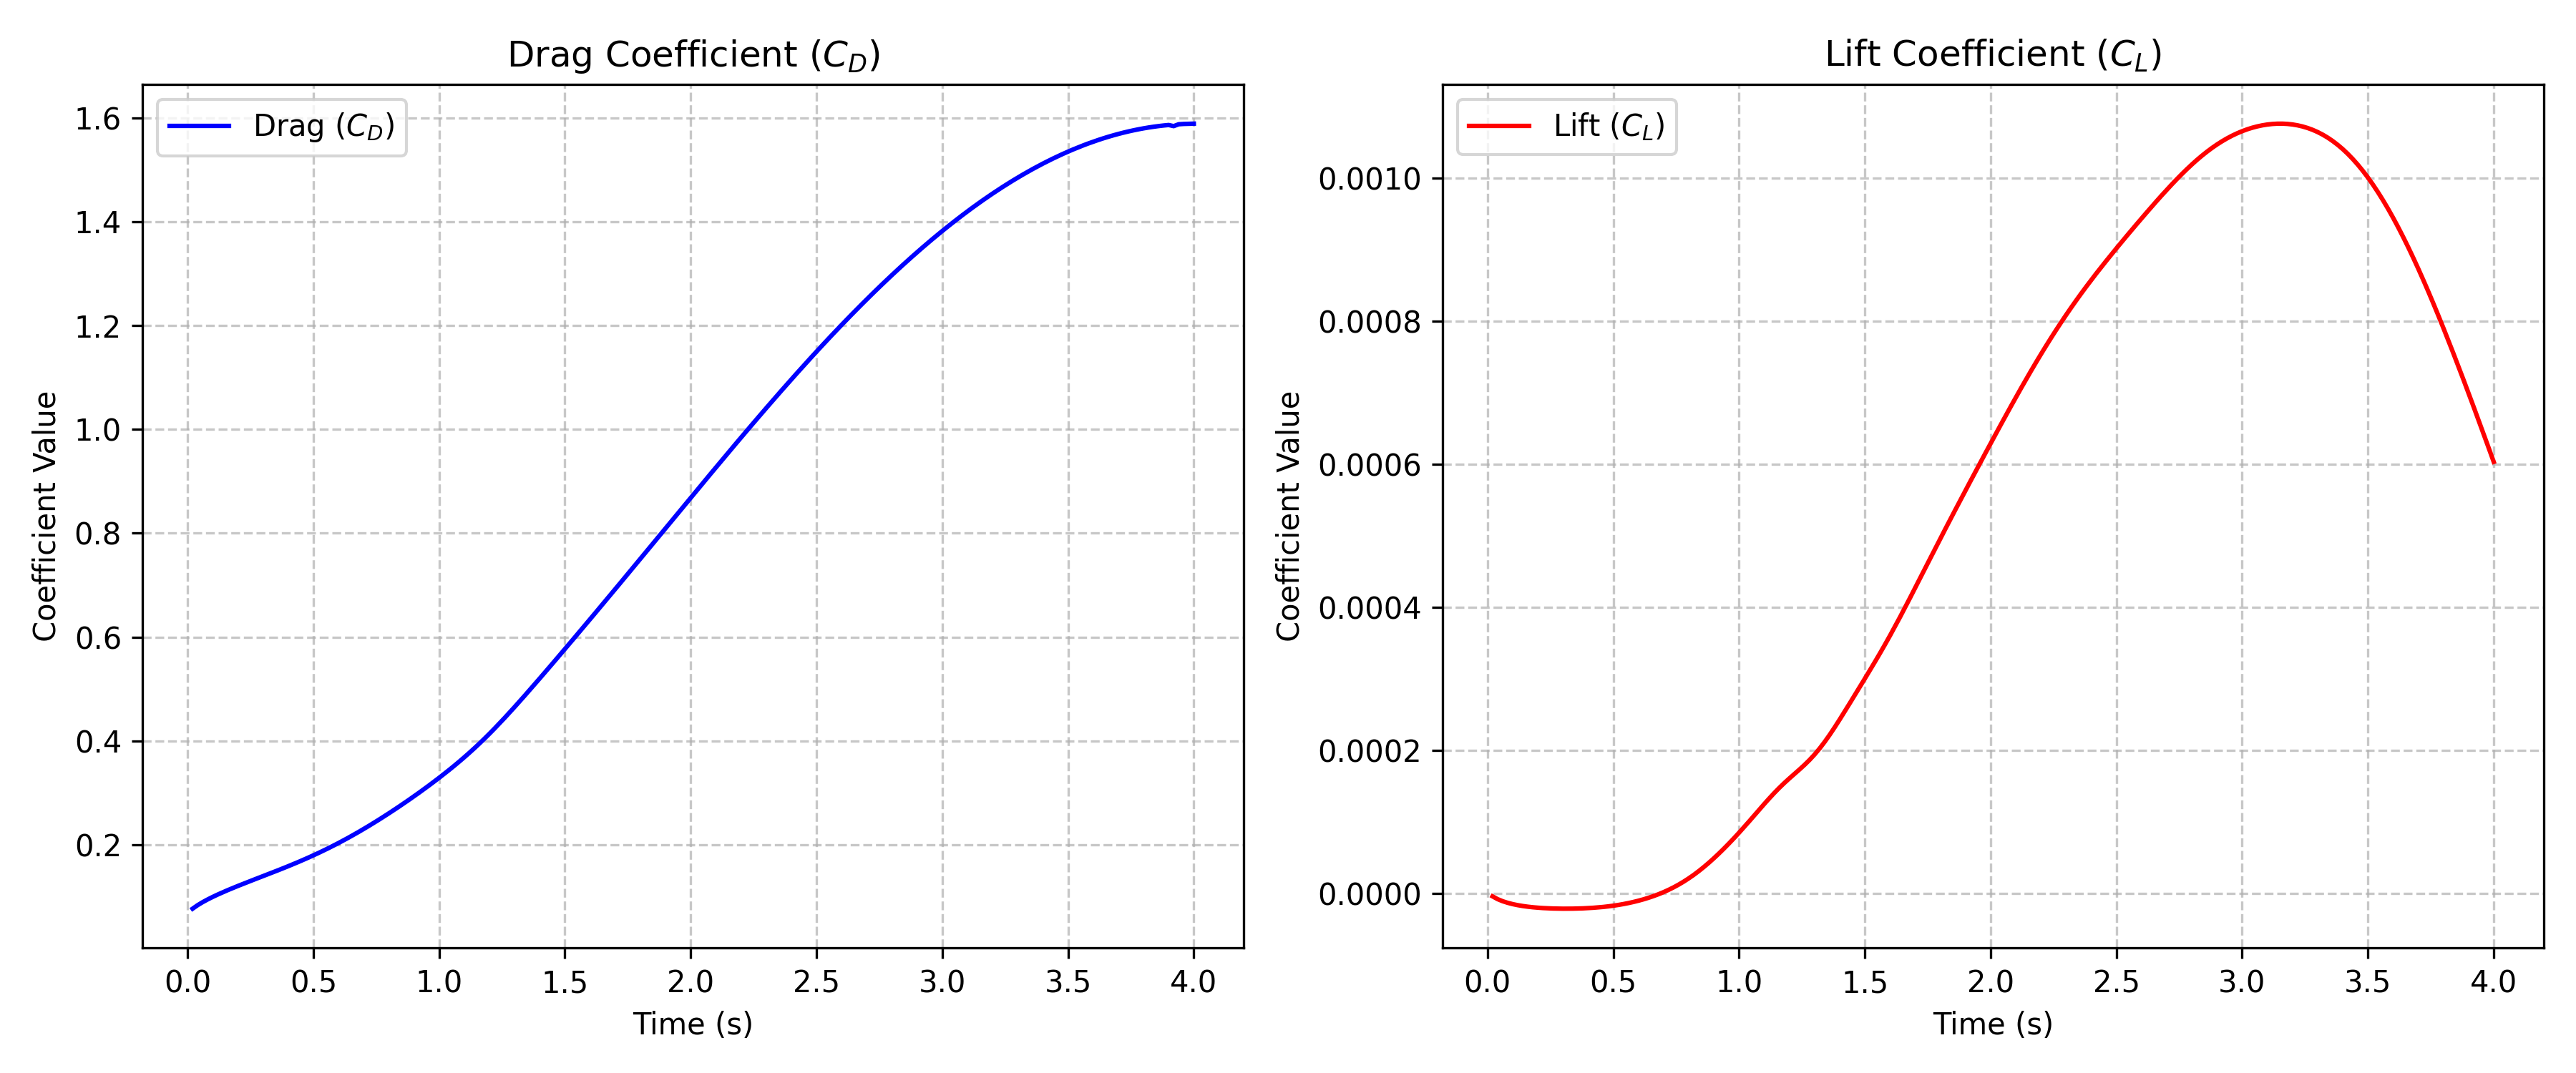
\includegraphics[width=0.75\textwidth]{cyl_drag_lift_coarse.png}
    }
    \\
    \subfloat[Cylinder: Fine mesh \label{fig:3d_3_cylinder_fine_dl}]{
        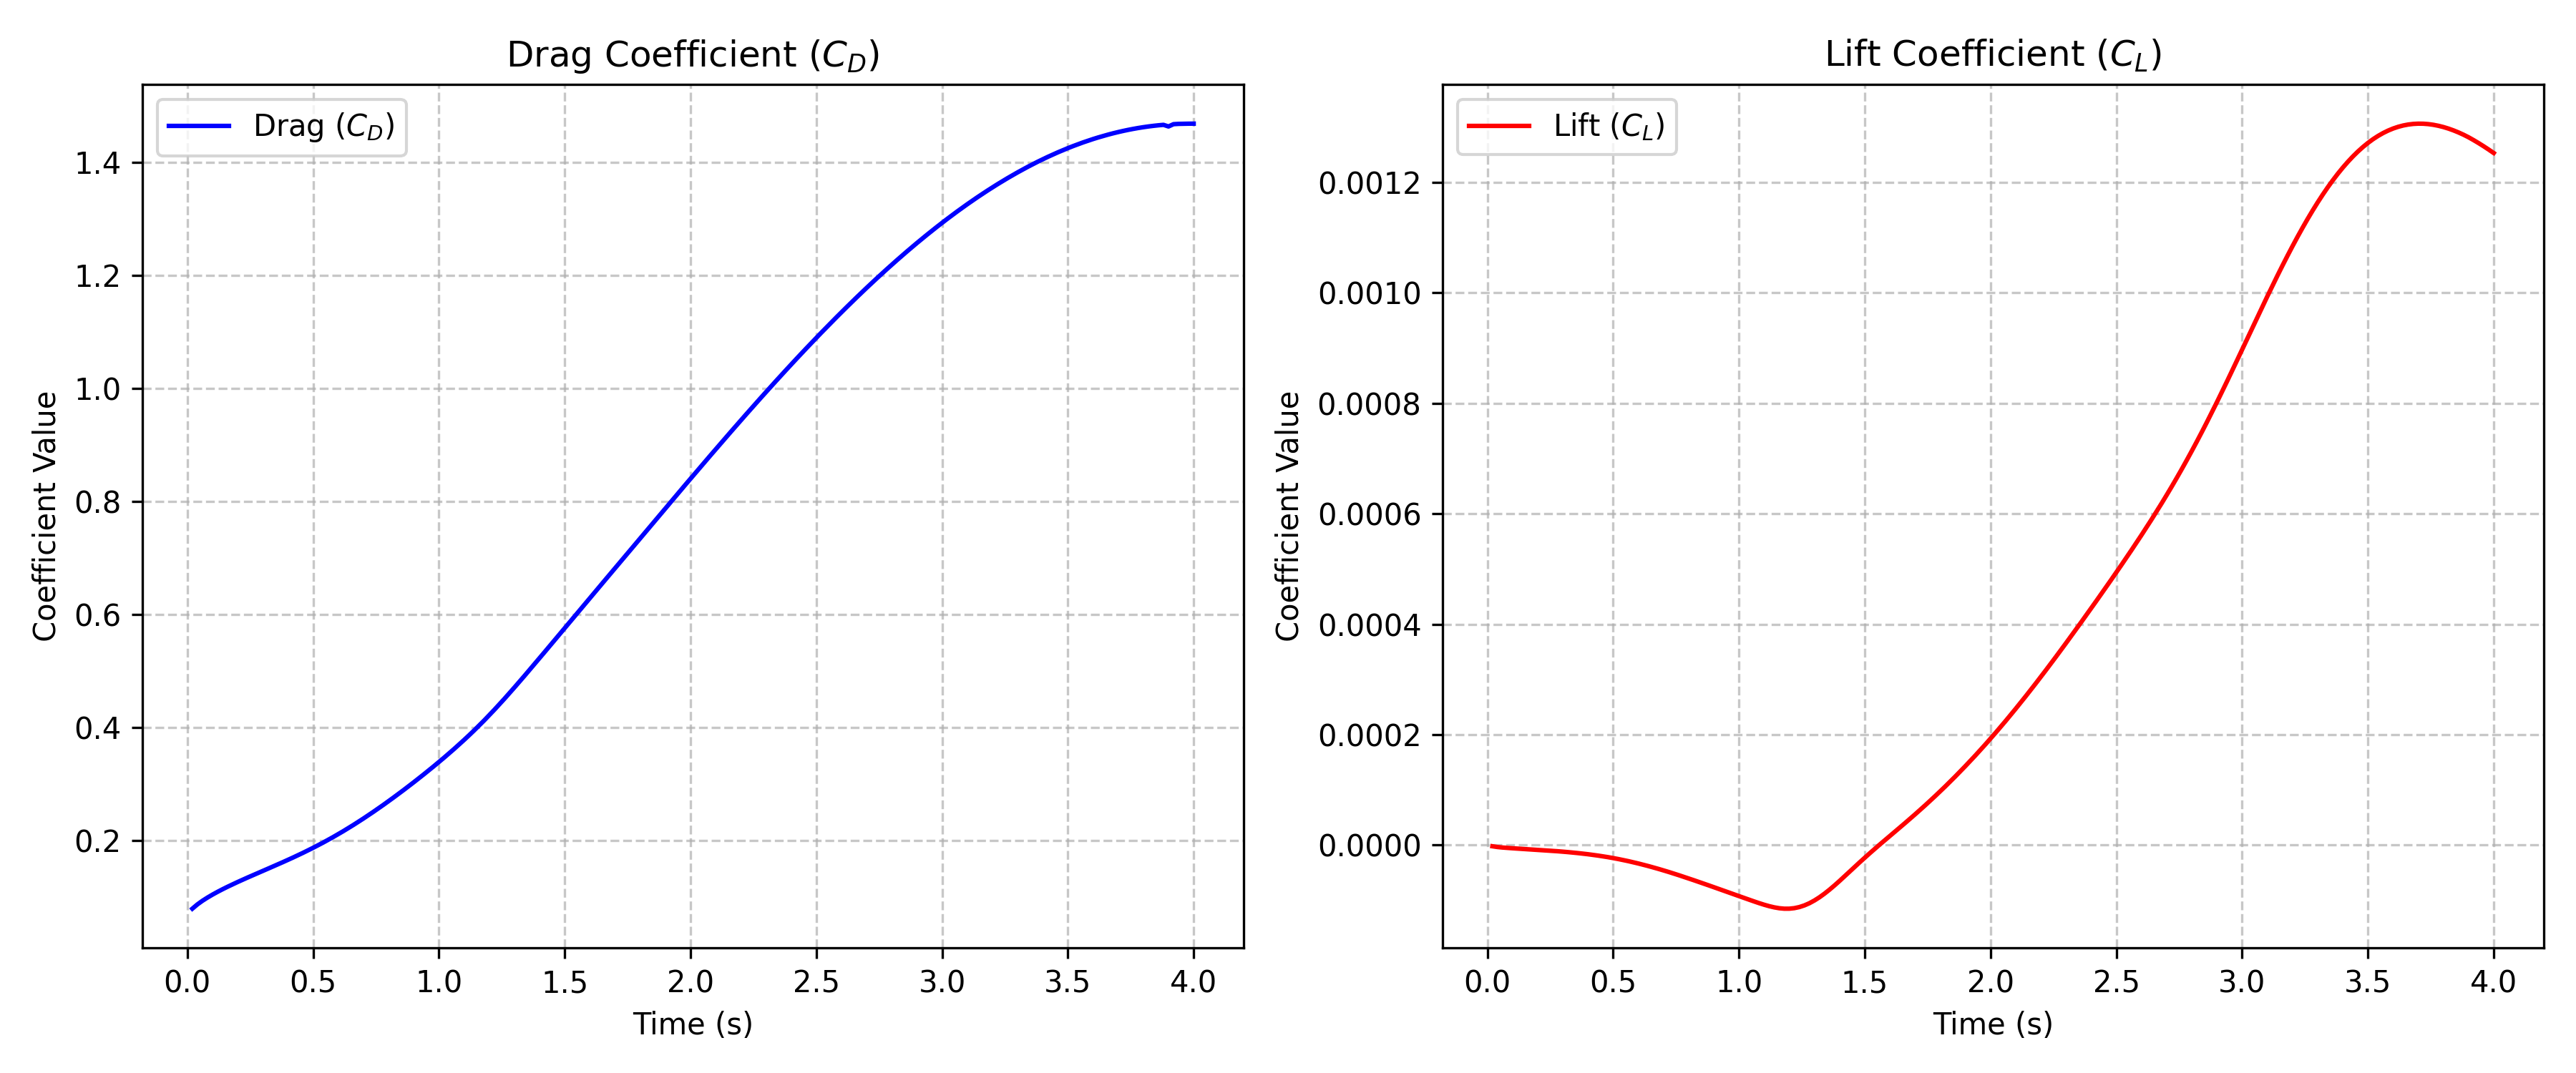
\includegraphics[width=0.75\textwidth]{fine_cyl_test3.png}
    }
    \\ \vspace{1em}
    % Cylinder Comparison
    \subfloat[Parallelepiped: Coarse mesh \label{fig:3d_3_parallelepiped_coarse_dl}]{
        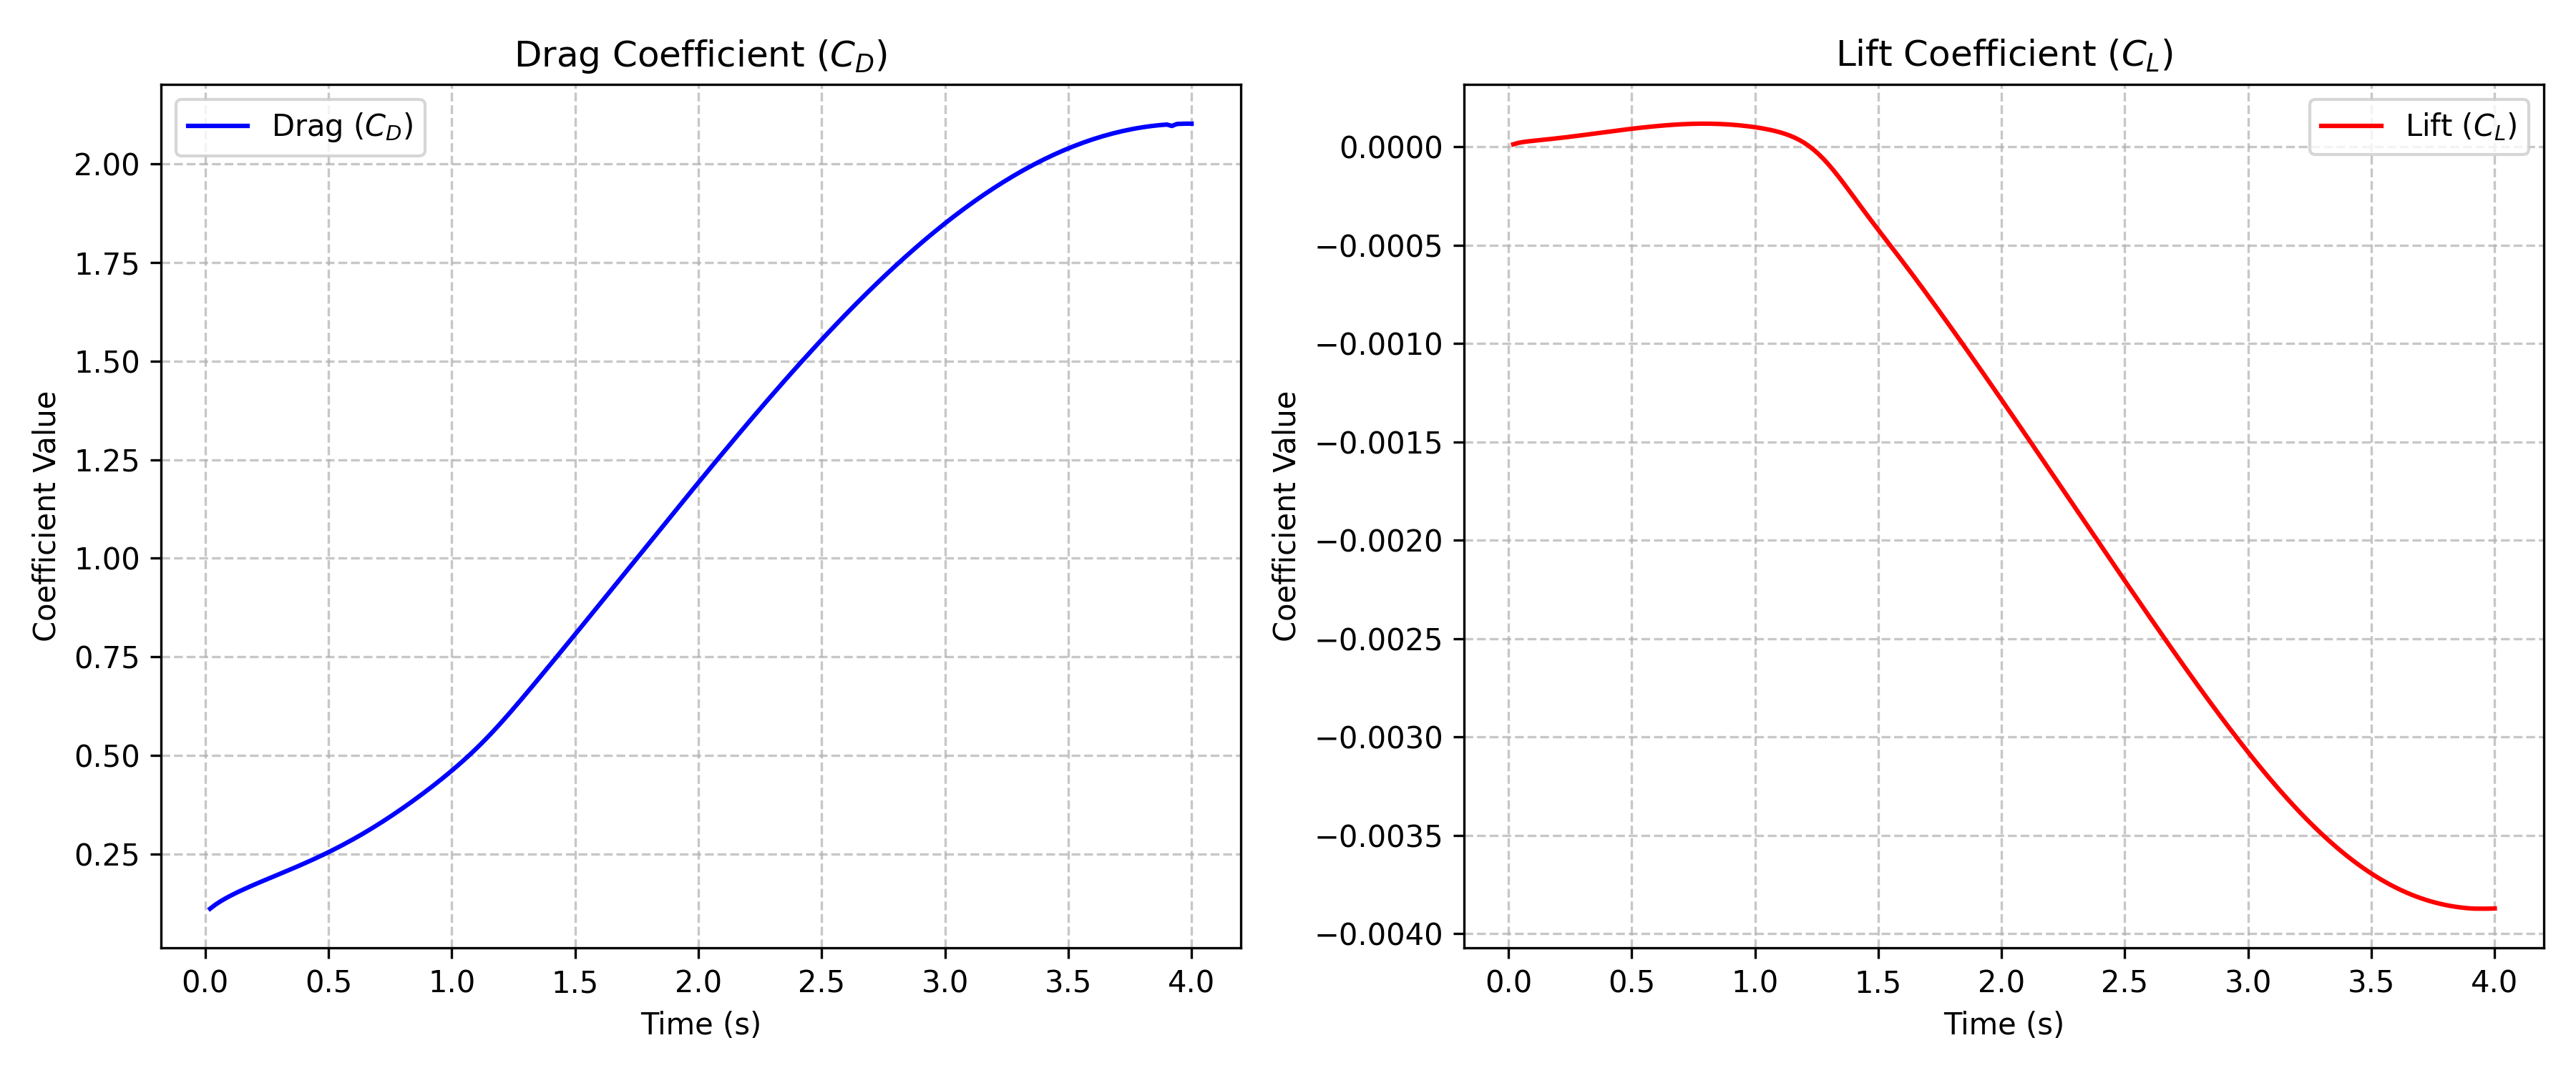
\includegraphics[width=0.75\textwidth]{par_drag_lift_coarse.png}
    }
    \\ 
    \subfloat[Parallelepiped: Fine mesh \label{fig:3d_3_parallelepiped_fine_dl}]{
        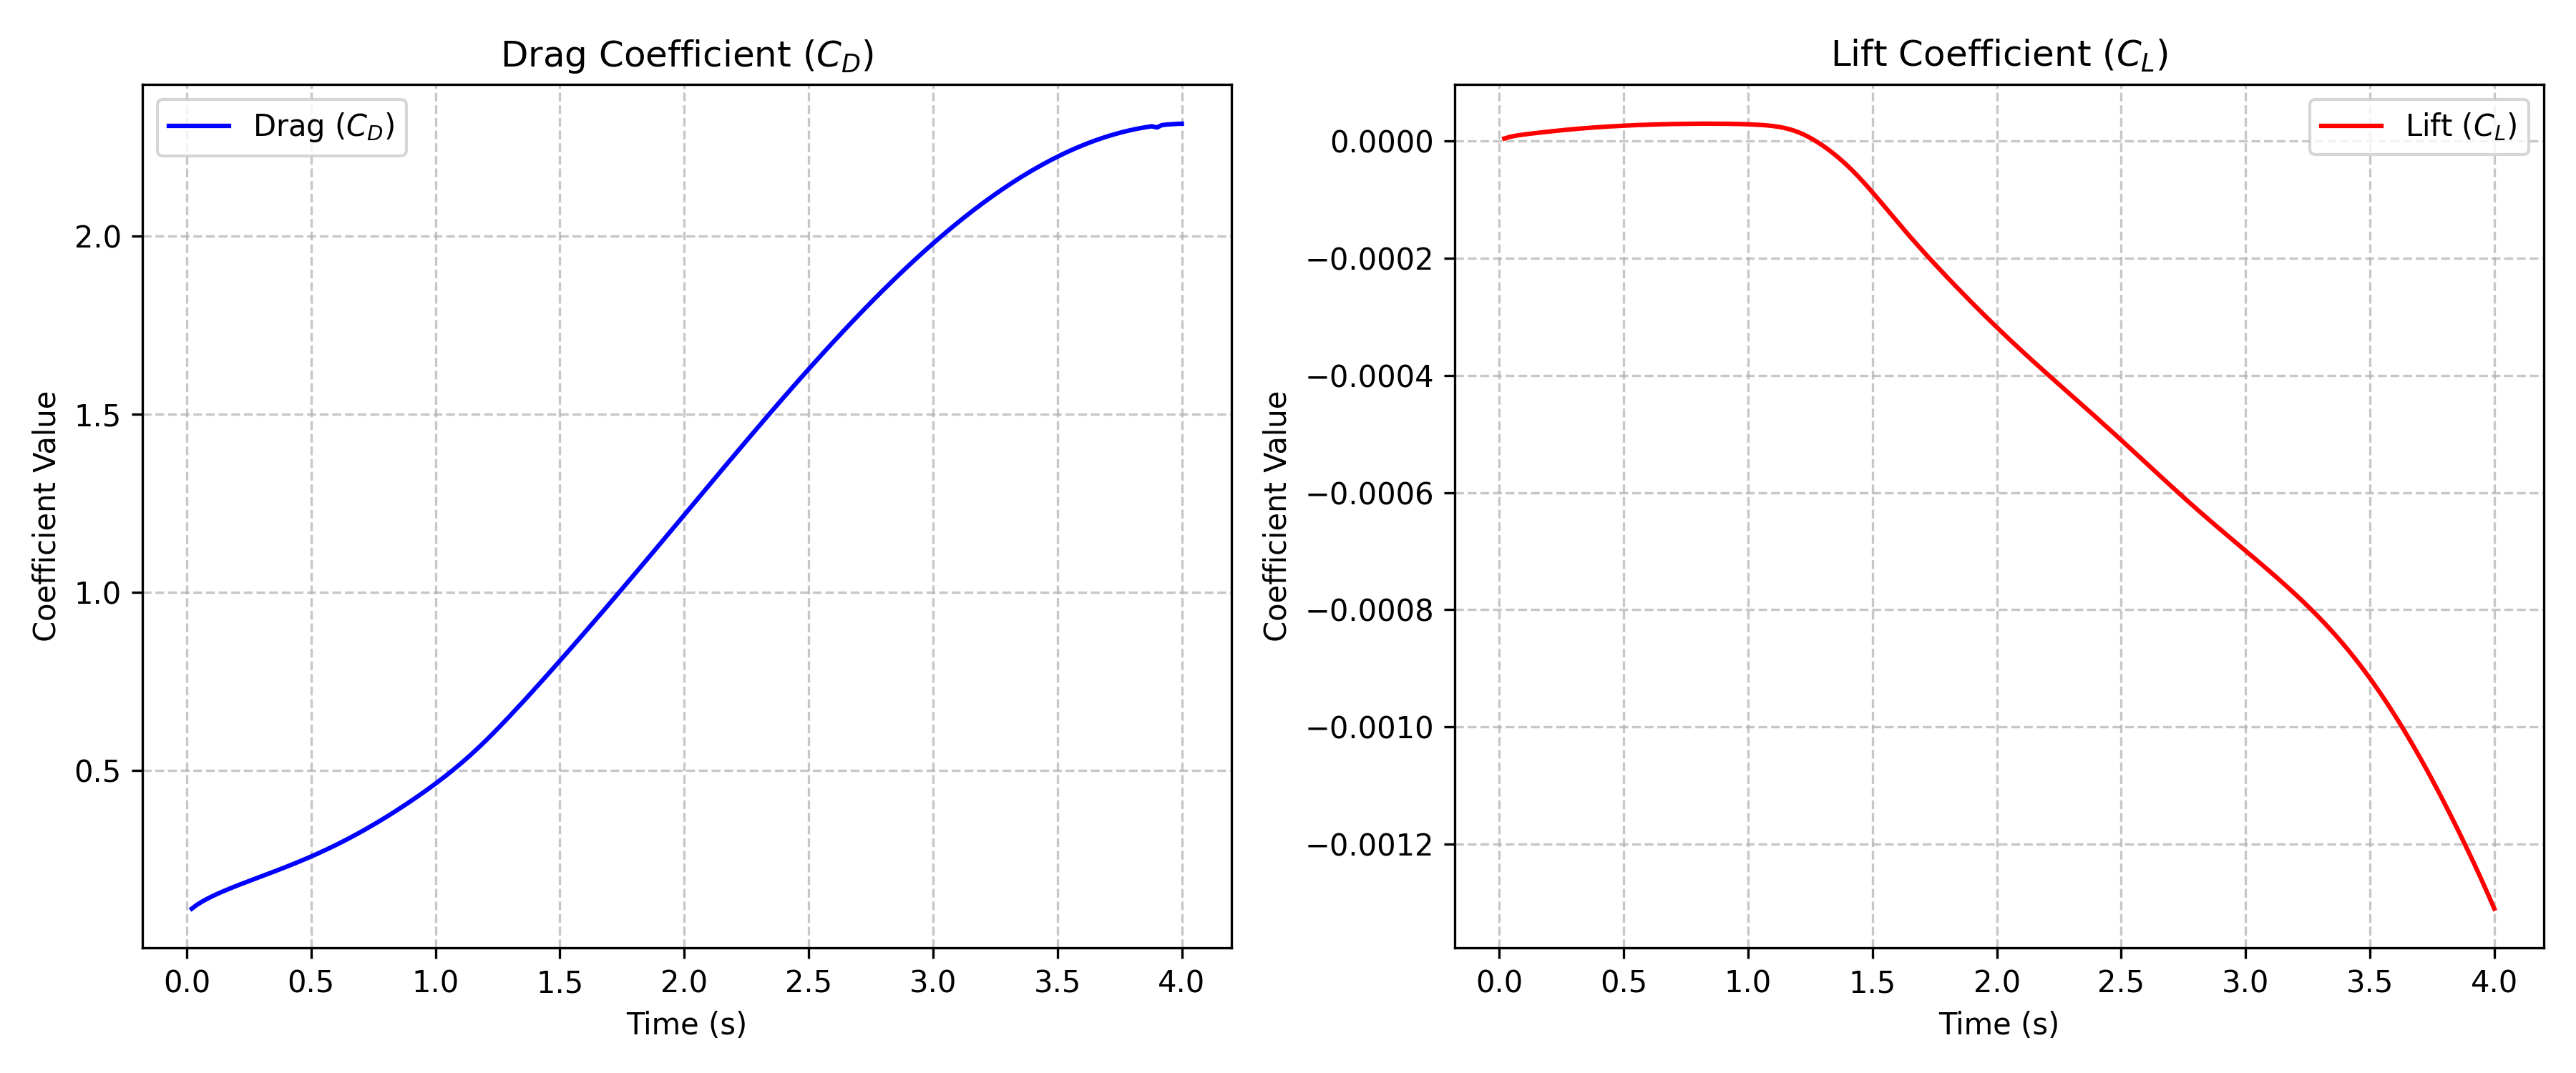
\includegraphics[width=0.75\textwidth]{frag_lift_par_fine.png}
    }
    \caption{Drag and Lift coefficients (Cylinder and Parallelepiped) for the 3D-3 unsteady test case.}
    \label{fig:3d_3_dl}
\end{figure}

%-----------------------------------------------
% CHORIN - TEMAM
%-----------------------------------------------
\begin{figure}[p]
    \centering
    % Cylinder Comparison
    \subfloat[]{
        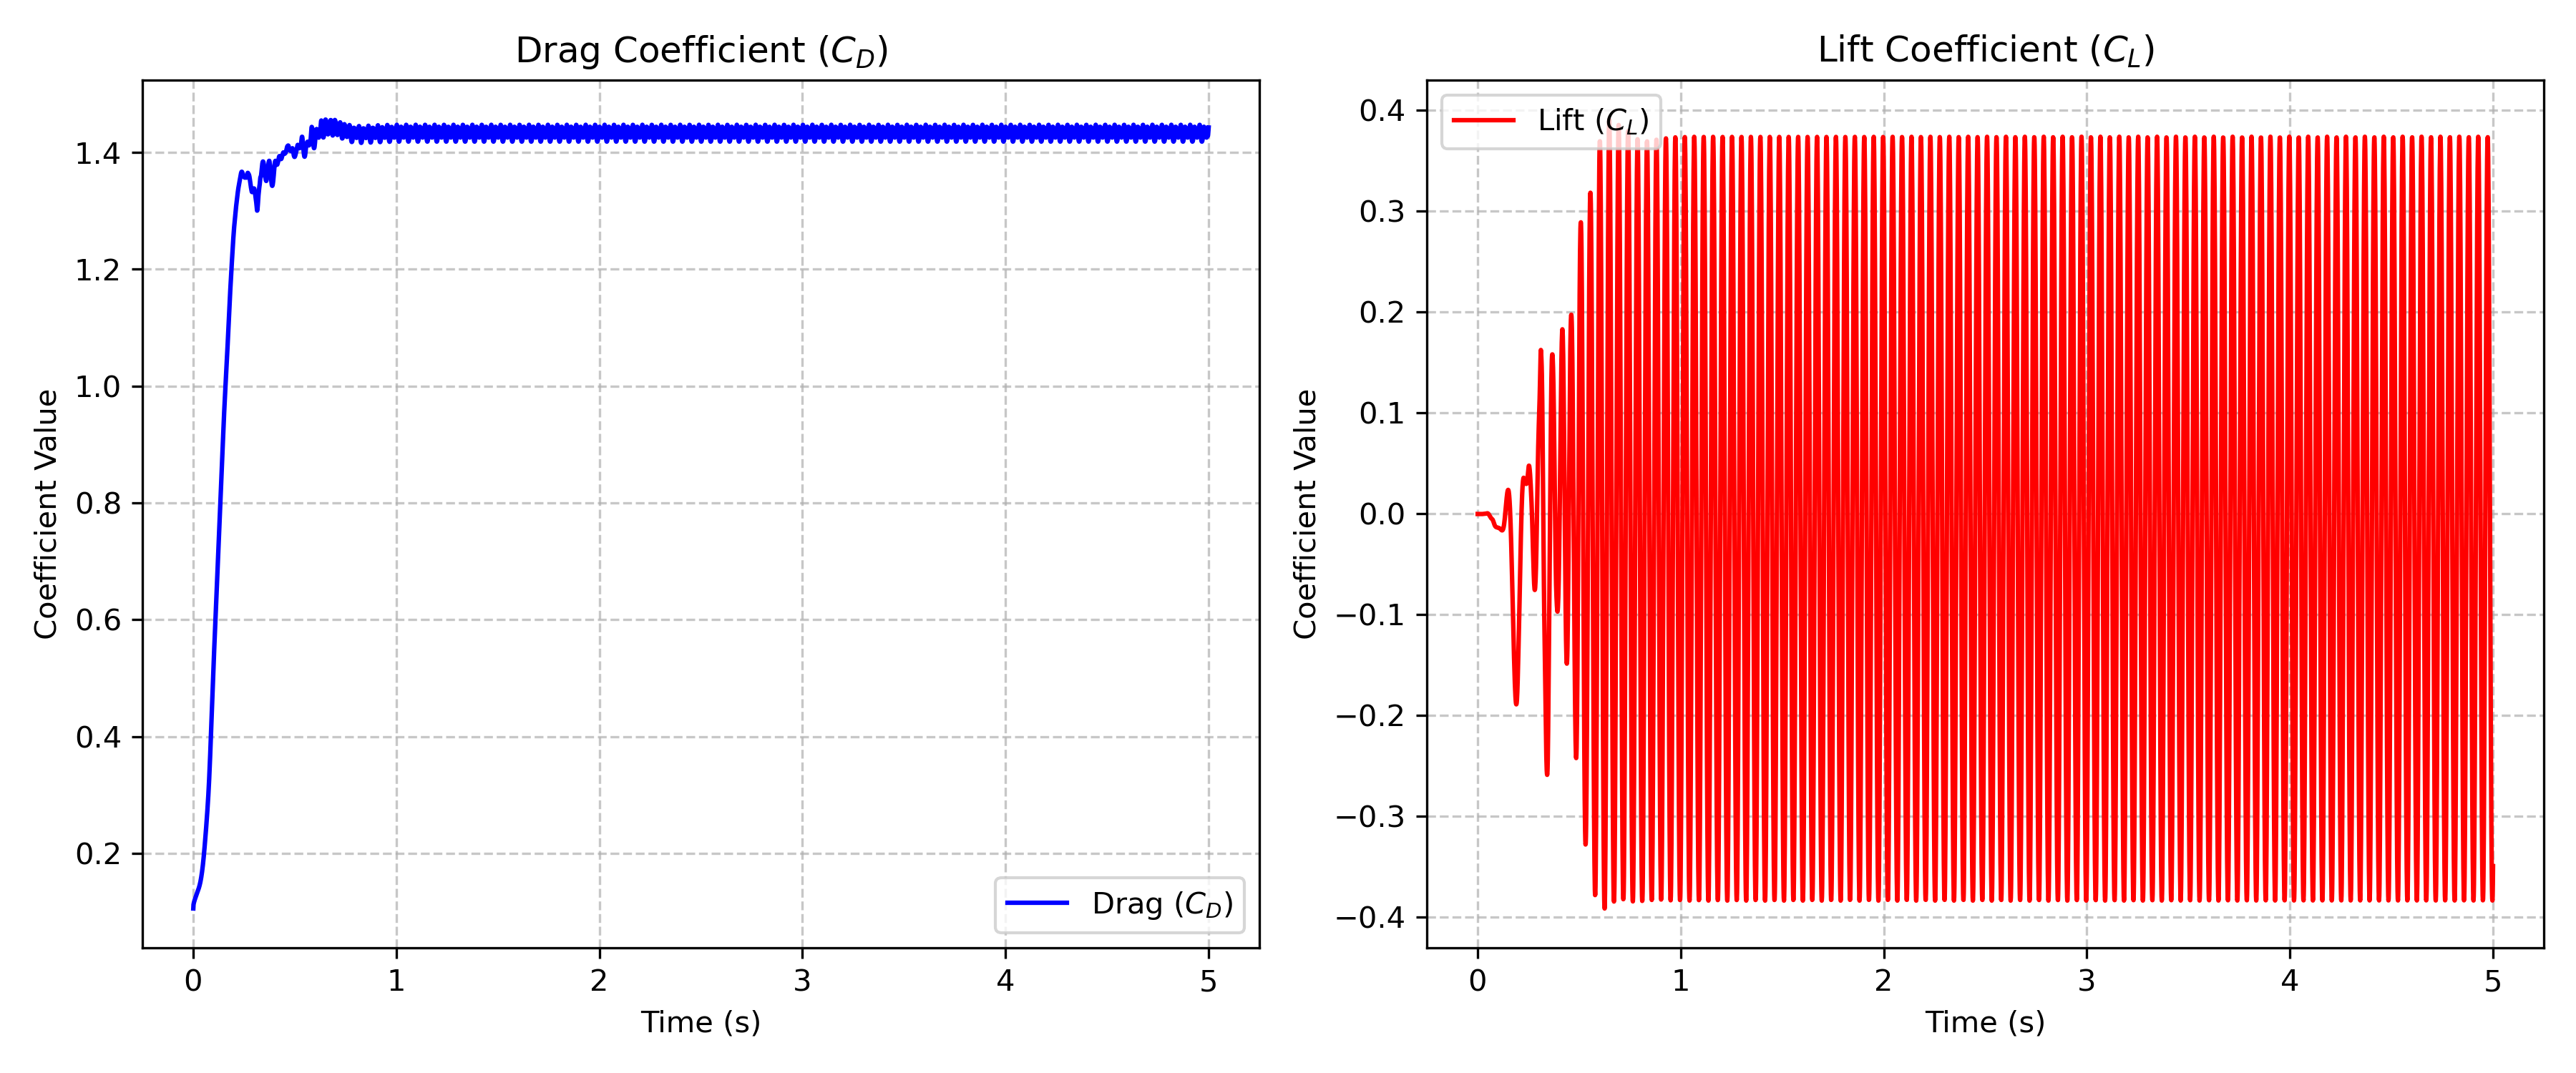
\includegraphics[width=\textwidth]{Images/Test_cases/2D/Re_1000_CT/coefficients_plot.png}
    }
    \caption{Drag and Lift coefficients for the $\Reynolds = 1000$ Chorin - Temam test case.}
    \label{fig:ct_dl}
\end{figure}




\FloatBarrier
\section{Simulation Screenshots}
\label{appendix:screenshots}
%-----------------------------------------------
% 2D TEST CASE 1
%-----------------------------------------------
\begin{figure}[h]
    \centering
    % Define a local command to keep widths consistent and code readable
    \newcommand{\gridwidth}{0.48\textwidth}

    % Row 1: velocity
    \subfloat[Velocity (Coarse) \label{fig:2d_1_coarse_velocity}]{
\includegraphics[width=\gridwidth]{Images/Test_cases/2D/Test_1/Screenshots/Coarse/t_5_velocity.png}} 
    \hfill
    \subfloat[Velocity (Fine) \label{fig:2d_1_fine_velocity}]{
\includegraphics[width=\gridwidth]{Images/Test_cases/2D/Test_1/Screenshots/Fine/t_5_velocity.png}} \\
    
    % Row 2: Pressure
    \subfloat[Pressure (Coarse) \label{fig:2d_1_coarse_pressure}]{
\includegraphics[width=\gridwidth]{Images/Test_cases/2D/Test_1/Screenshots/Coarse/t_5_pressure.png}} 
    \hfill
    \subfloat[Pressure (Fine) \label{fig:2d_1_fine_pressure}]{
\includegraphics[width=\gridwidth]{Images/Test_cases/2D/Test_1/Screenshots/Fine/t_5_pressure.png}} \\

    \caption{Instantaneous velocity and pressure fields at $t = 5s$ for the coarse (left) and fine (right) meshes in the 2D-1 steady test case.}
    \label{fig:2d_1_velocity_pressure_snapshots}
\end{figure}

%-----------------------------------------------
% 2D TEST CASE 1
%-----------------------------------------------
\begin{figure}[h]
    \centering
    % Define a local command to keep widths consistent and code readable
    \newcommand{\gridwidth}{0.48\textwidth}

    % Row 1: velocity
    \subfloat[Velocity (Coarse) \label{fig:2d_2_coarse_velocity}]{
\includegraphics[width=\gridwidth]{Images/Test_cases/2D/Test_2/Screenshots/Coarse/t_5_velocity.png}} 
    \hfill
    \subfloat[Velocity (Fine) \label{fig:2d_2_fine_velocity}]{
\includegraphics[width=\gridwidth]{Images/Test_cases/2D/Test_2/Screenshots/Fine/t_5_velocity.png}} \\
    
    % Row 2: Pressure
    \subfloat[Pressure (Coarse) \label{fig:2d_2_coarse_pressure}]{
\includegraphics[width=\gridwidth]{Images/Test_cases/2D/Test_2/Screenshots/Coarse/t_5_pressure.png}} 
    \hfill
    \subfloat[Pressure (Fine) \label{fig:2d_2_fine_pressure}]{
\includegraphics[width=\gridwidth]{Images/Test_cases/2D/Test_2/Screenshots/Fine/t_5_pressure.png}} \\

    \caption{Instantaneous velocity and pressure fields at $t = 5s$ for the coarse (left) and fine (right) meshes in the 2D-2 steady test case.}
    \label{fig:2d_2_velocity_pressure_snapshots}
\end{figure}

%-----------------------------------------------
% 2D TEST CASE 3
%-----------------------------------------------
\begin{figure}[p]
    \centering

    \foreach \t in {2,4,6,8} {

        \subfloat[$t=\t$, coarse]{%
            \includegraphics[width=0.48\textwidth]{Images/Test_cases/2D/Test_3/Screeshots/Coarse/t_\t_velocity.png}%
        }
        \hfill
        \subfloat[$t=\t$, fine]{%
            \includegraphics[width=0.48\textwidth]{Images/Test_cases/2D/Test_3/Screeshots/Fine/t_\t_velocity.png}%
        }

        \vspace{0.3cm}
    }

    \caption{Instantaneous velocity fields at selected times for the coarse (left) and fine (right) meshes in the 2D-3 unsteady test case.}
    \label{fig:2d_3_velocity_snapshots}
\end{figure}
\begin{figure}[p]
    \centering

    \foreach \t in {2,4,6,8} {

        \subfloat[$t=\t$, coarse]{%
            \includegraphics[width=0.48\textwidth]{Images/Test_cases/2D/Test_3/Screeshots/Coarse/t_\t_pressure.png}%
        }
        \hfill
        \subfloat[$t=\t$, fine]{%
            \includegraphics[width=0.48\textwidth]{Images/Test_cases/2D/Test_3/Screeshots/Fine/t_\t_pressure.png}%
        }

        \vspace{0.3cm}
    }

    \caption{Instantaneous pressure fields at selected times for the coarse (left) and fine (right) meshes in the 2D-3 unsteady test case.}
    \label{fig:2d_3_pressure_snapshots}
\end{figure}

%-------------------------------------------------------------
% 3D TEST CASE 1
%-------------------------------------------------------------
% --- SIMULATION GRID: VELOCITY & PRESSURE ---
\begin{figure}[p]
    \centering
    % Define a local command to keep widths consistent and code readable
    \newcommand{\gridwidth}{0.48\textwidth}

    % Row 1: Cylinder Velocity
    \subfloat[Cylinder Velocity (Coarse) \label{fig:3d_1_cylinder_coarse_velocity}]{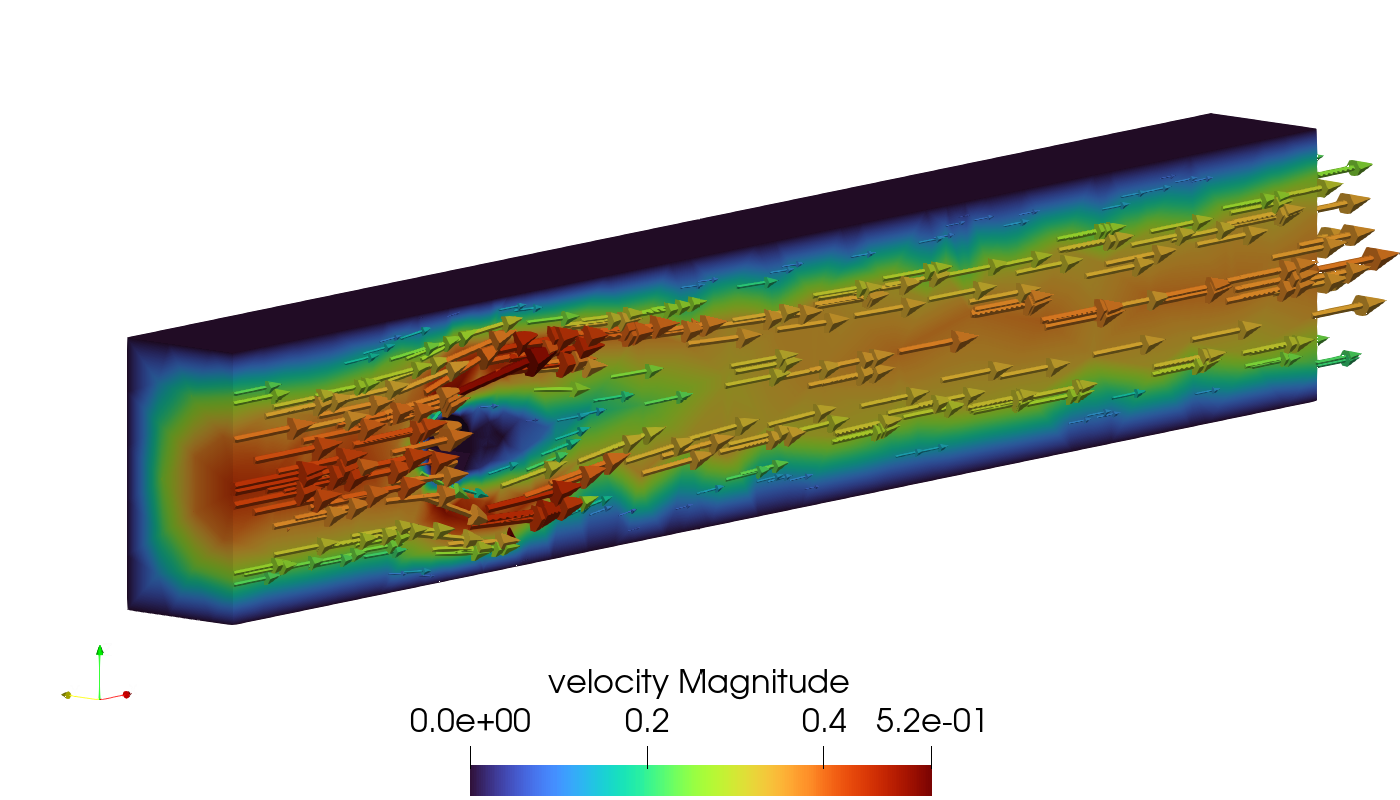
\includegraphics[width=\gridwidth]{t_4_cylinder_coarse_velocity.png}} 
    \hfill
    \subfloat[Cylinder Velocity (Fine) \label{fig:3d_1_cylinder_fine_velocity}]{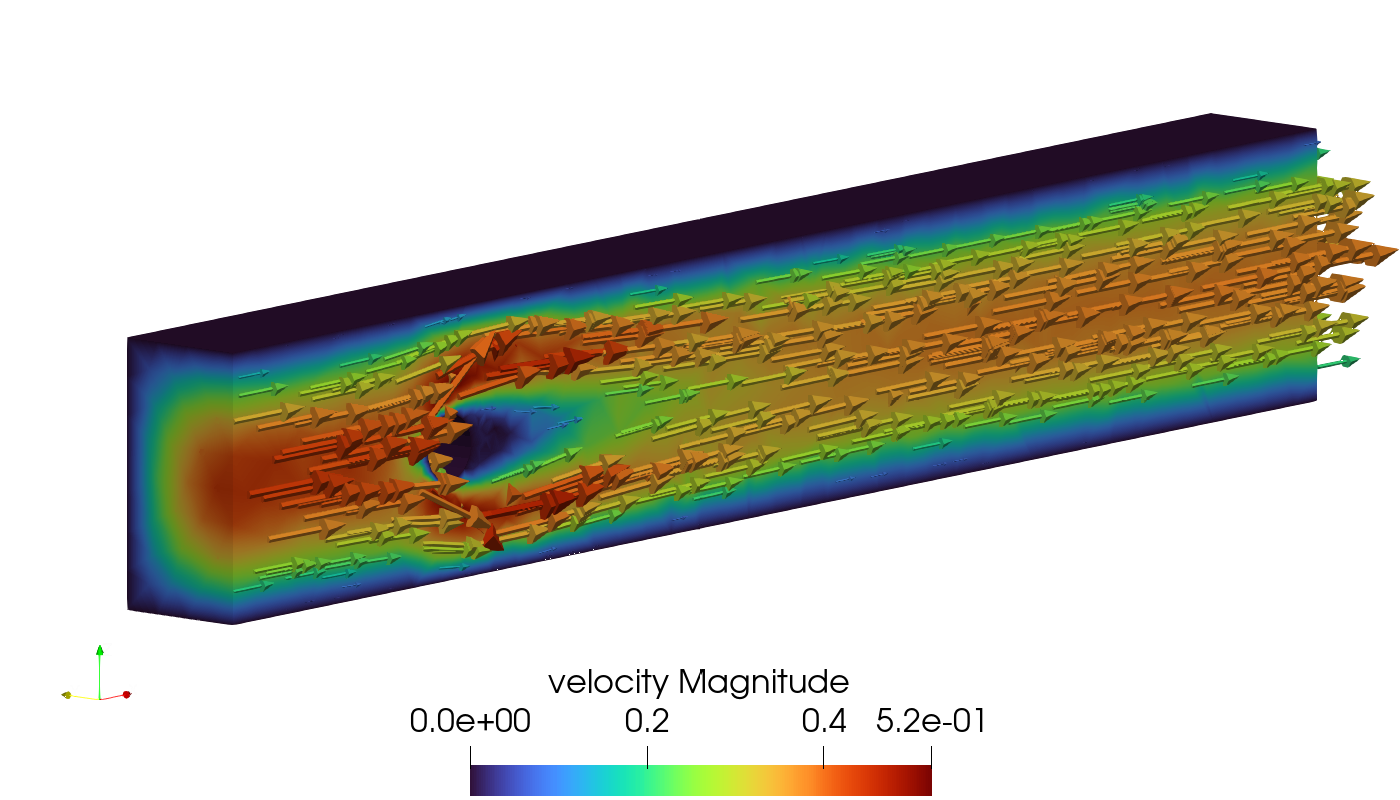
\includegraphics[width=\gridwidth]{t_4_cylinder_fine_velocity.png}} \\
    
    % Row 2: Cylinder Pressure
    \subfloat[Cylinder Pressure (Coarse) \label{fig:3d_1_cylinder_coarse_pressure}]{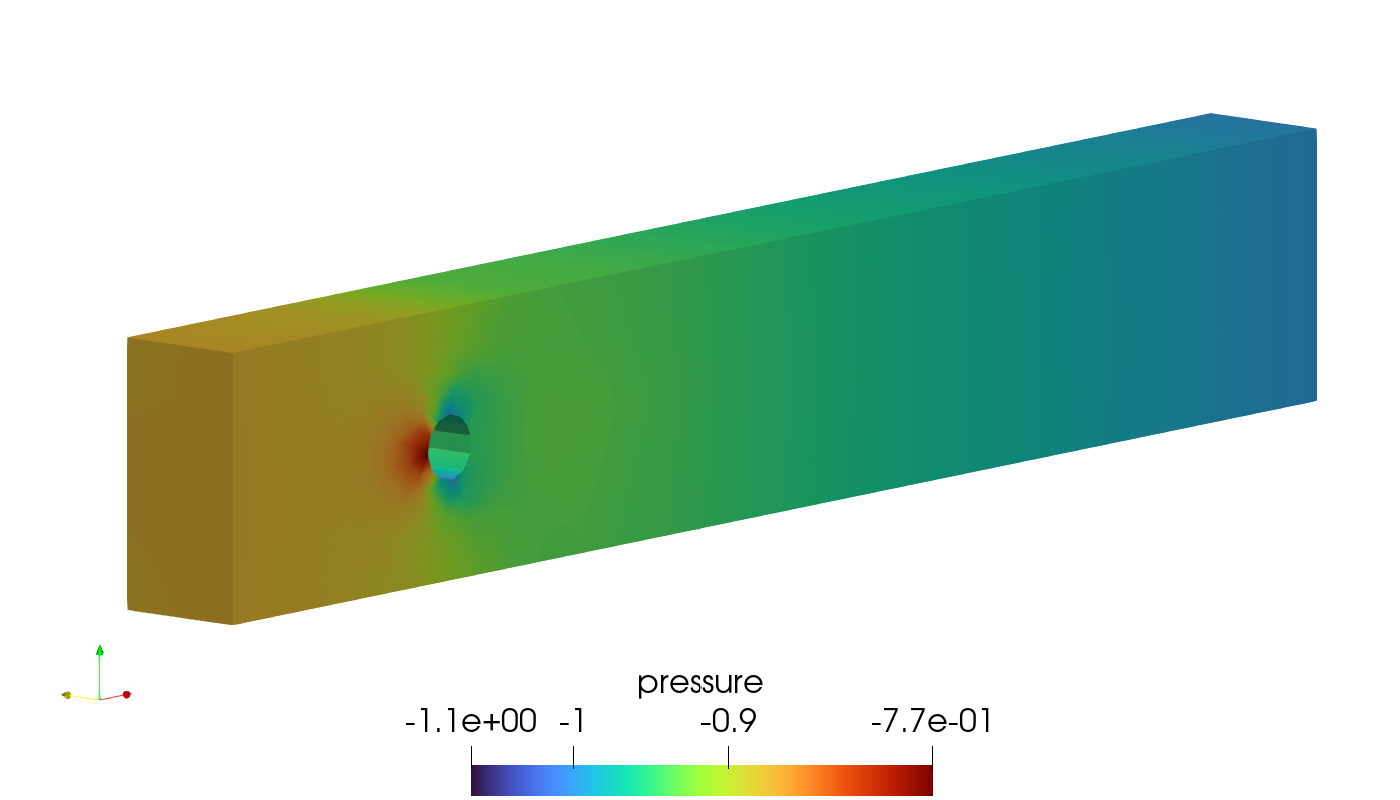
\includegraphics[width=\gridwidth]{t_4_cylinder_coarse_pressure.png}} 
    \hfill
    \subfloat[Cylinder Pressure (Fine) \label{fig:3d_1_cylinder_fine_pressure}]{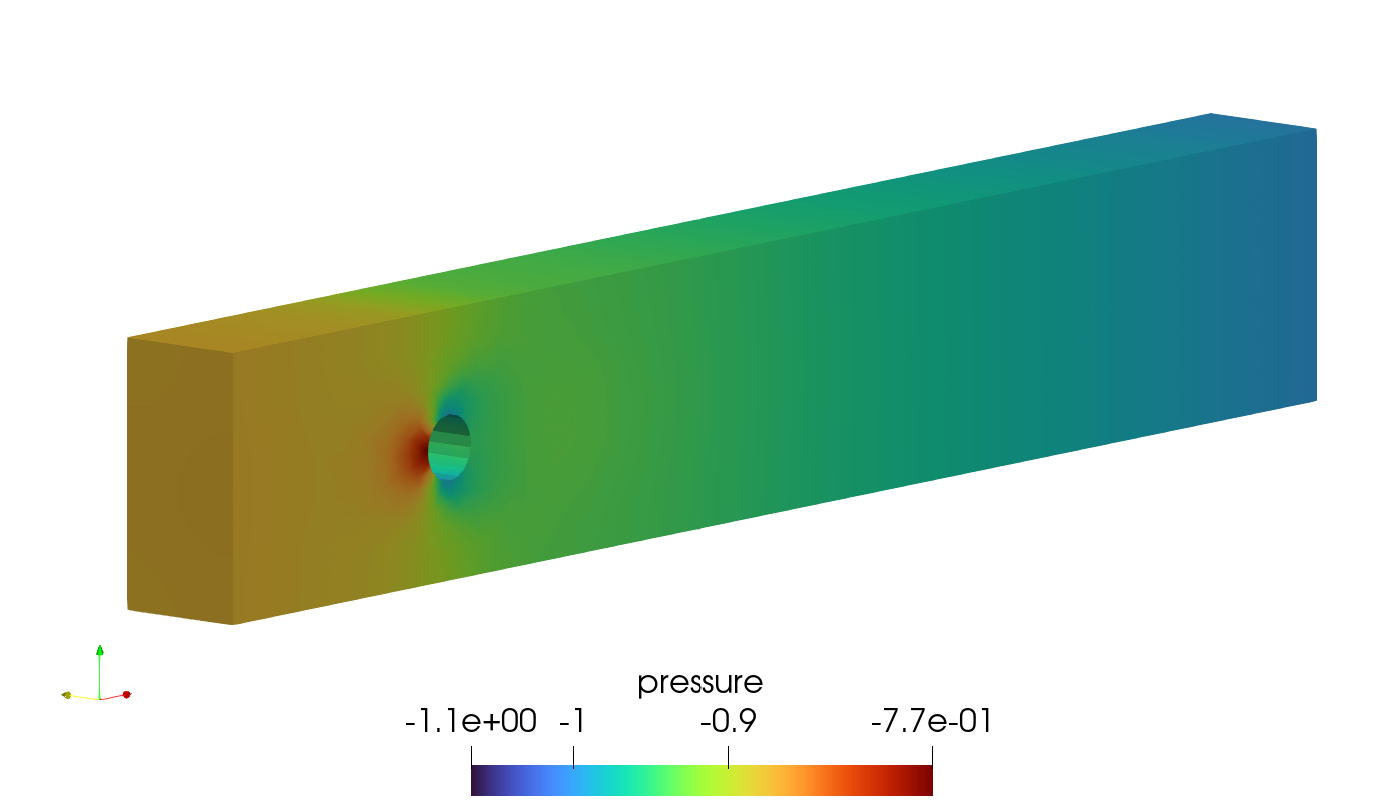
\includegraphics[width=\gridwidth]{t_4_cylinder_fine_pressure.png}} \\
    
    % Row 3: Parallelepiped Velocity
    \subfloat[Parallelepiped Velocity (Coarse)  \label{fig:3d_1_parallelepiped_coarse_velocity}]{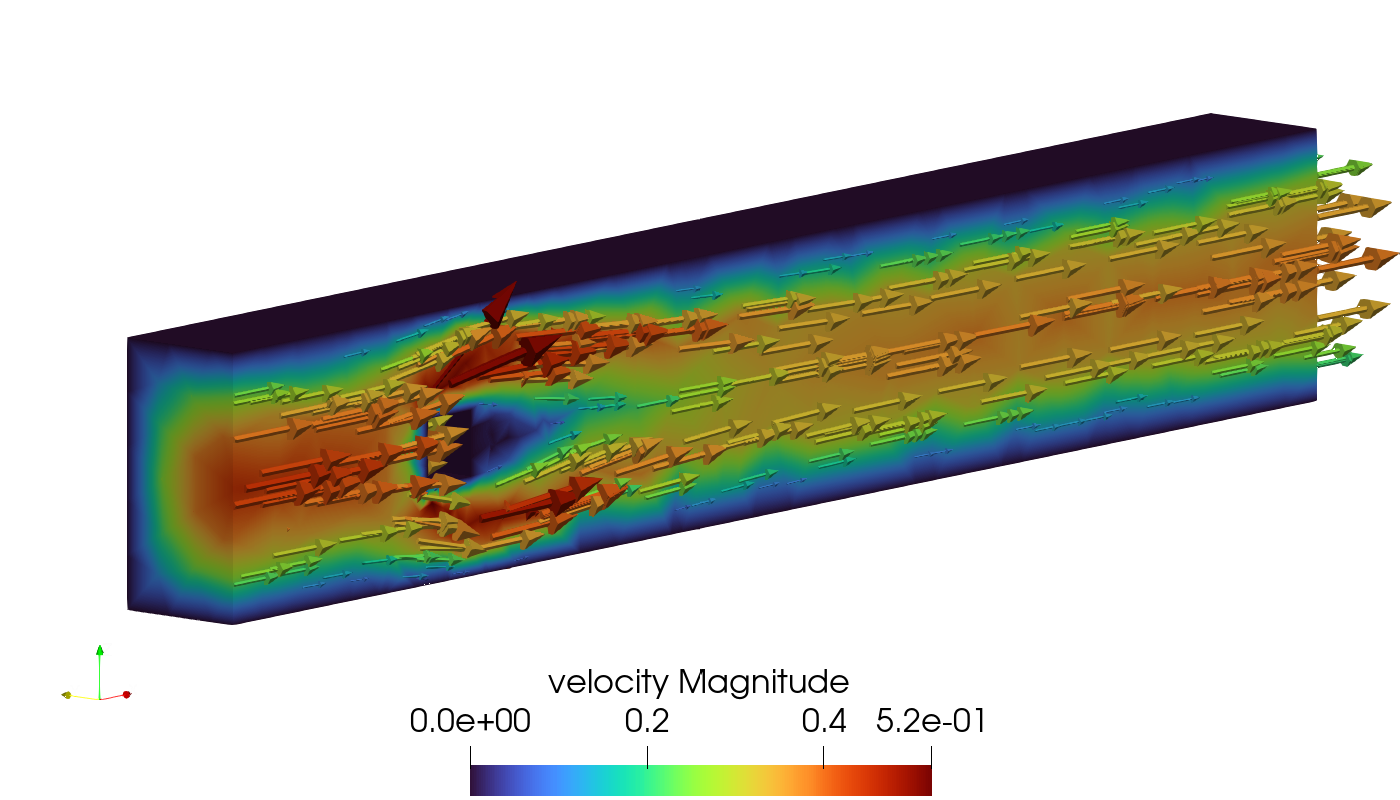
\includegraphics[width=\gridwidth]{t_4_parallelepiped_coarse_velocity.png}} 
    \hfill
    \subfloat[Parallelepiped Velocity (Fine) \label{fig:3d_1_parallelepiped_fine_velocity}]{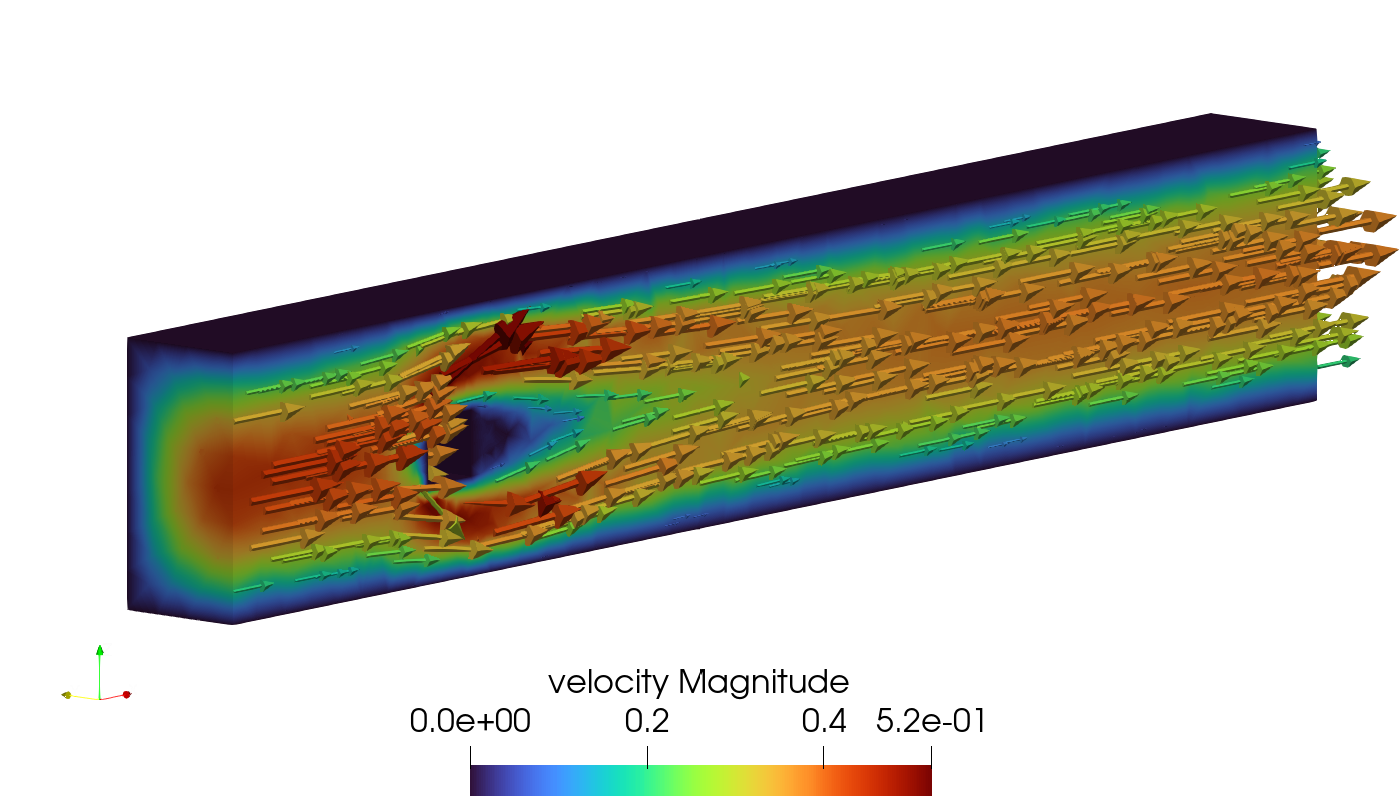
\includegraphics[width=\gridwidth]{t_4_parallelepiped_fine_velocity.png}} \\
    
    % Row 4: Parallelepiped Pressure
    \subfloat[Parallelepiped Pressure (Coarse) \label{fig:3d_1_parallelepiped_coarse_pressure}]{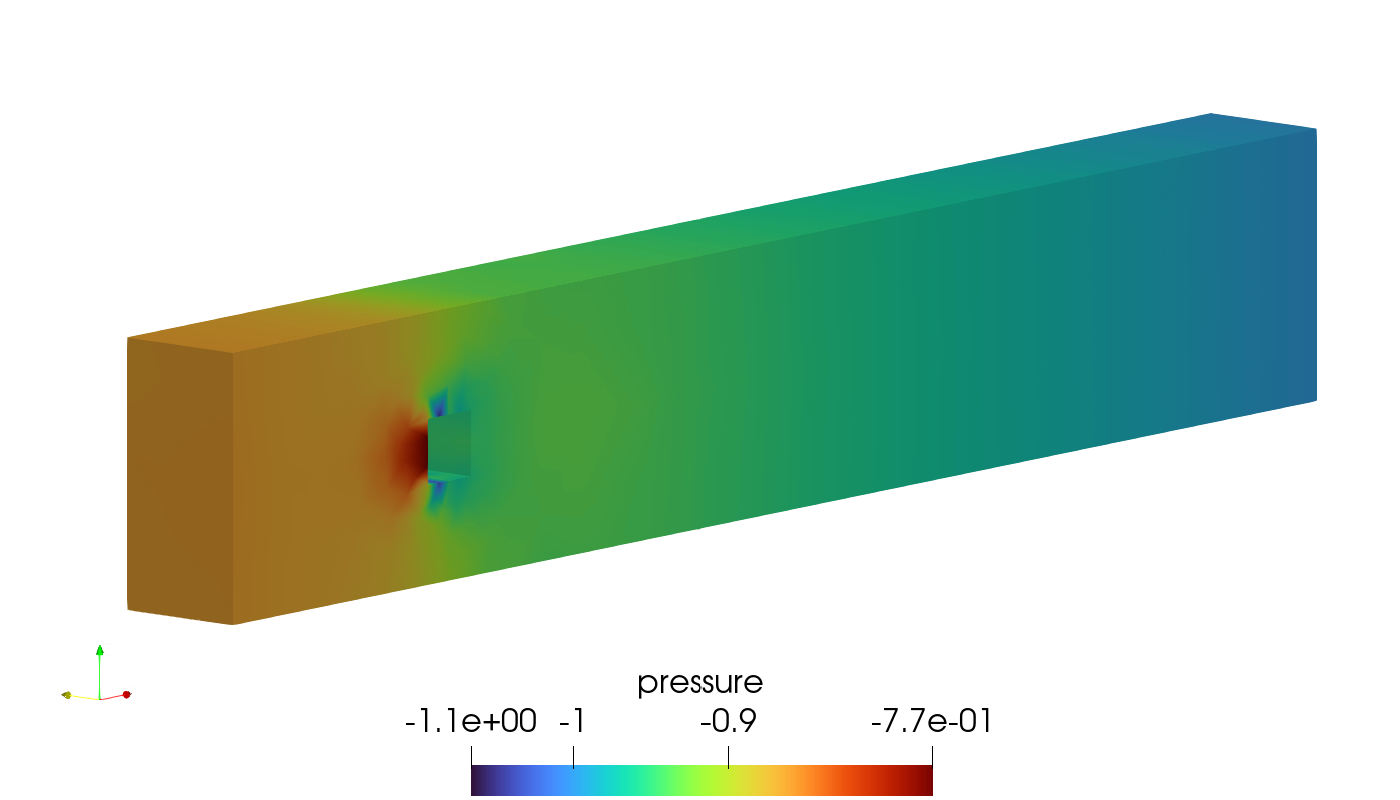
\includegraphics[width=\gridwidth]{t_4_parallelepiped_coarse_pressure.png}} 
    \hfill
    \subfloat[Parallelepiped Pressure (Fine)\label{fig:3d_1_parallelepiped_fine_pressure}]{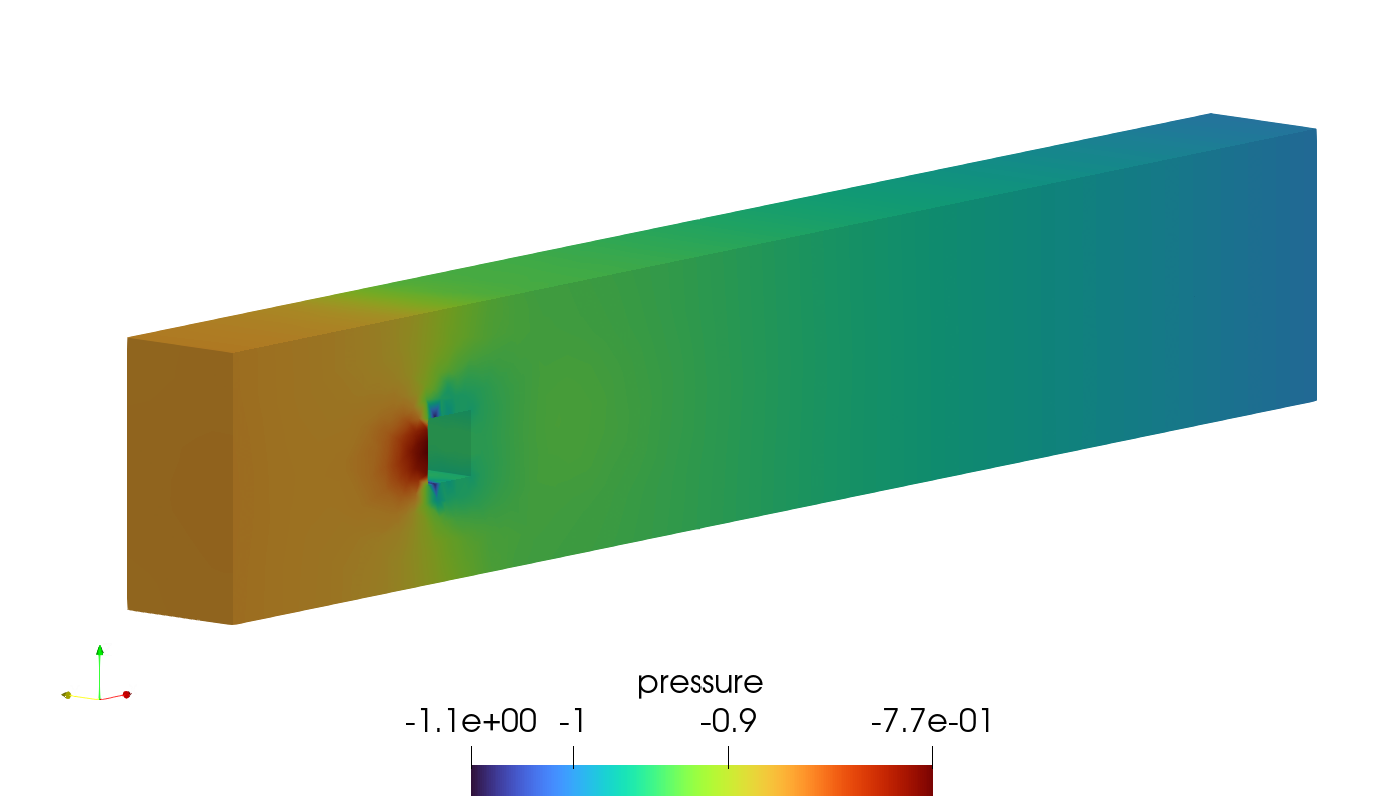
\includegraphics[width=\gridwidth]{Images/Test_cases/3D/Test_1/Screenshots/t_4_parallelepiped_fine_pressure.png}}

    \caption{Instantaneous velocity and pressure fields for square and circular section obstacles at $t = 4s$ for the coarse (left) and fine (right) meshes in the 3D-1 steady test case.}
    \label{fig:3d_1_velocity__pressure_snapshots}
\end{figure}


%-------------------------------------------------------------
% 3D TEST CASE 2
%-------------------------------------------------------------
% --- SIMULATION GRID: VELOCITY & PRESSURE ---
\begin{figure}[p]
    \centering
    % Define a local command to keep widths consistent and code readable
    \newcommand{\gridwidth}{0.48\textwidth}

    % Row 1: Cylinder Velocity
    \subfloat[Cylinder Velocity (Fine)]{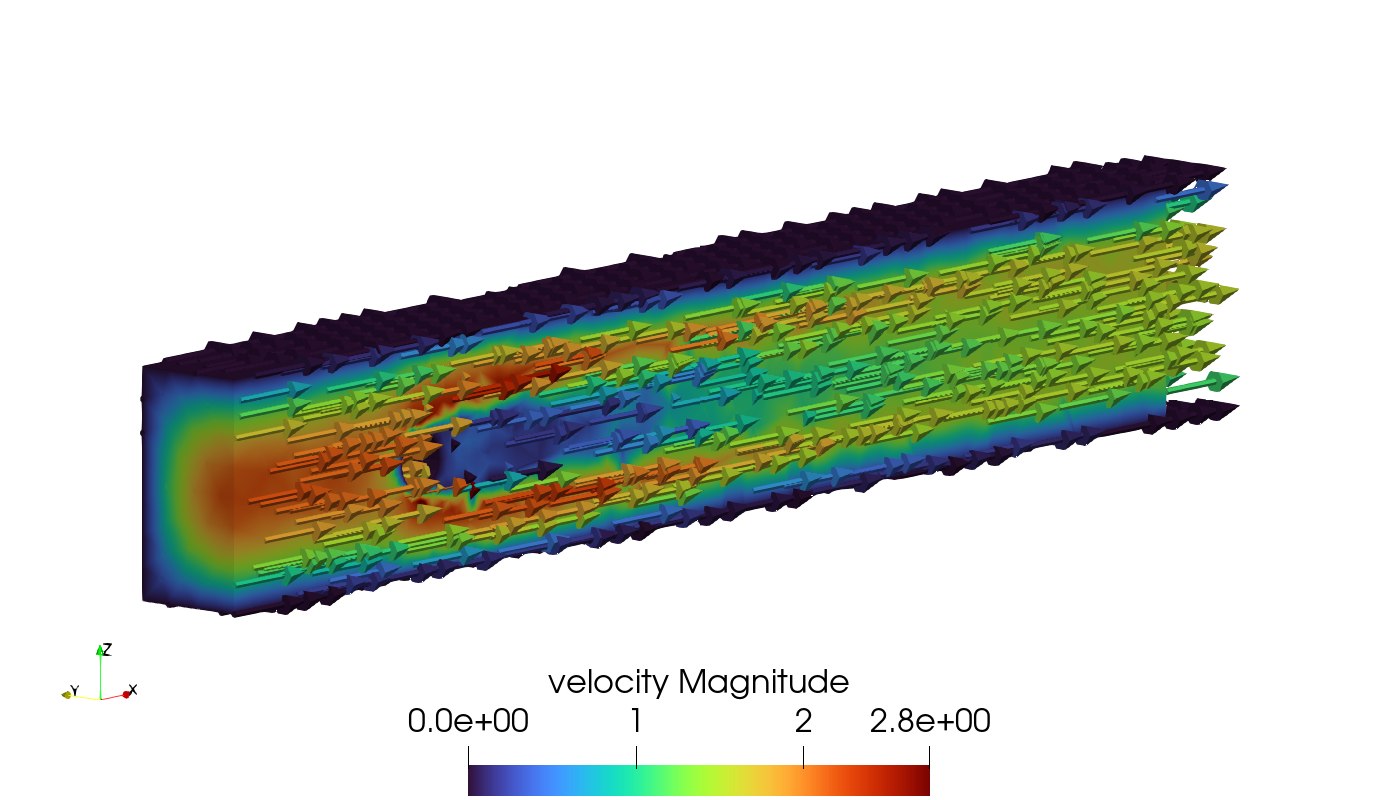
\includegraphics[width=\gridwidth]{glyph_test2_fine.png}} 
    \hfill
    \subfloat[Cylinder Pressure (Fine)]{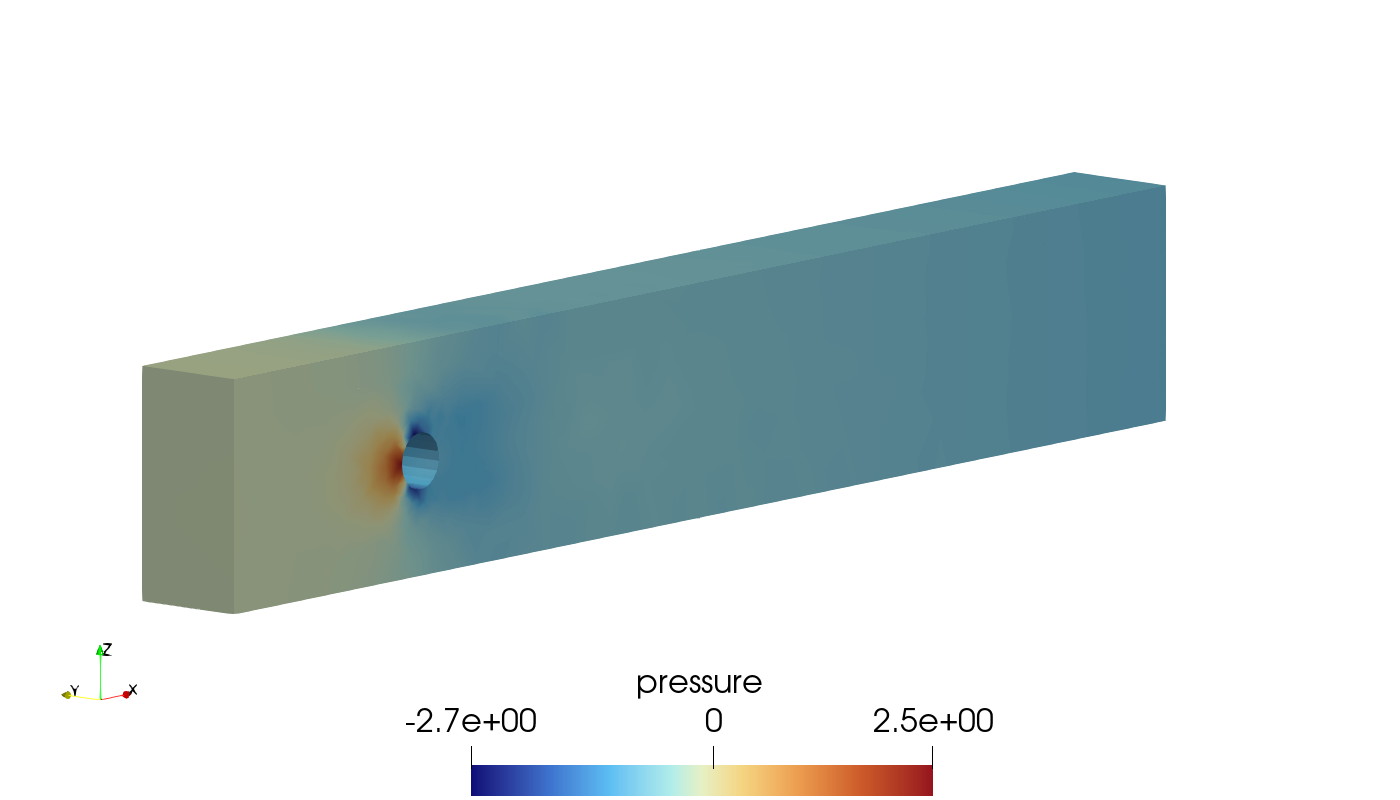
\includegraphics[width=\gridwidth]{pres_test2_cyl.png}} \\

    \subfloat[Cylinder Velocity (Fine)]{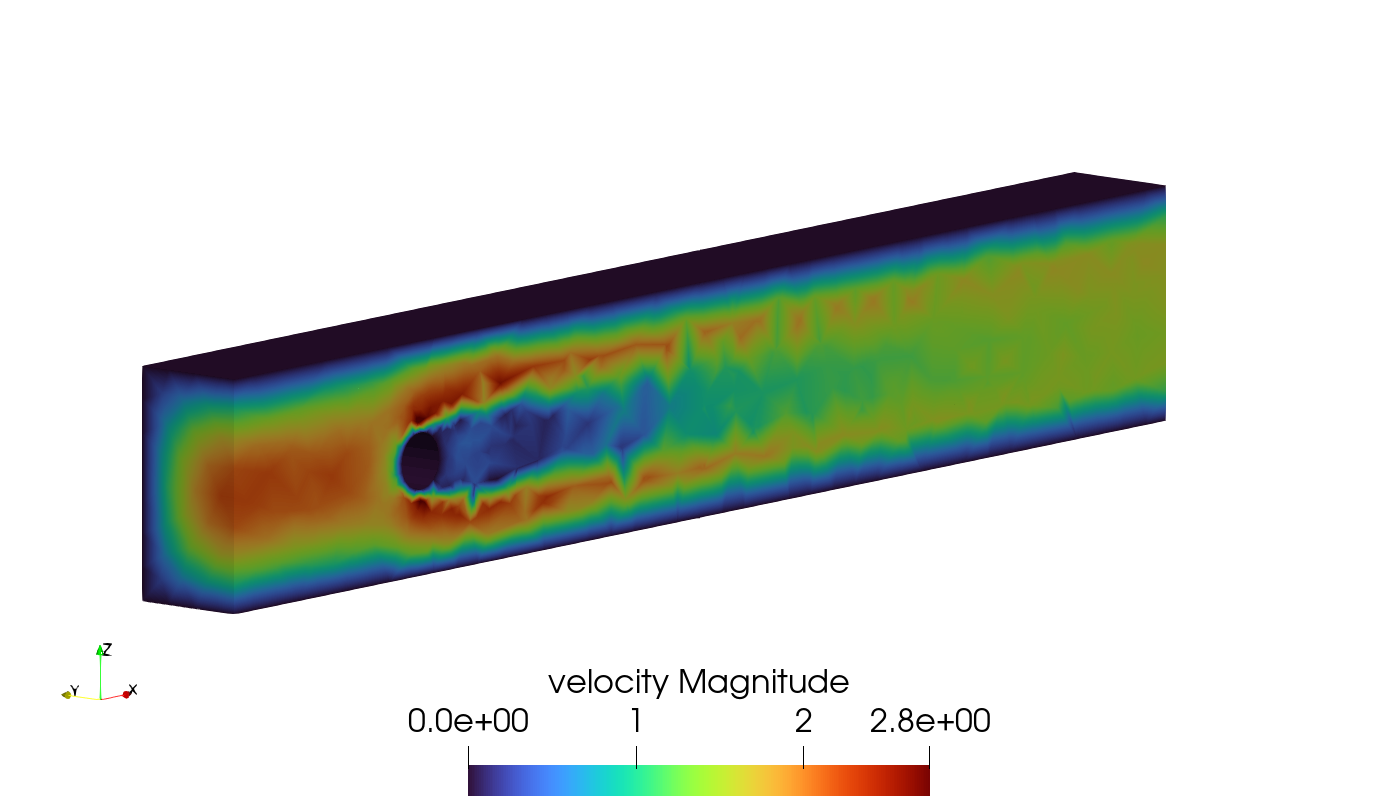
\includegraphics[width=\gridwidth]{vel_test2_cyl.png}} 
    \hfill
    \subfloat[Cylinder Pressure (Coarse)]{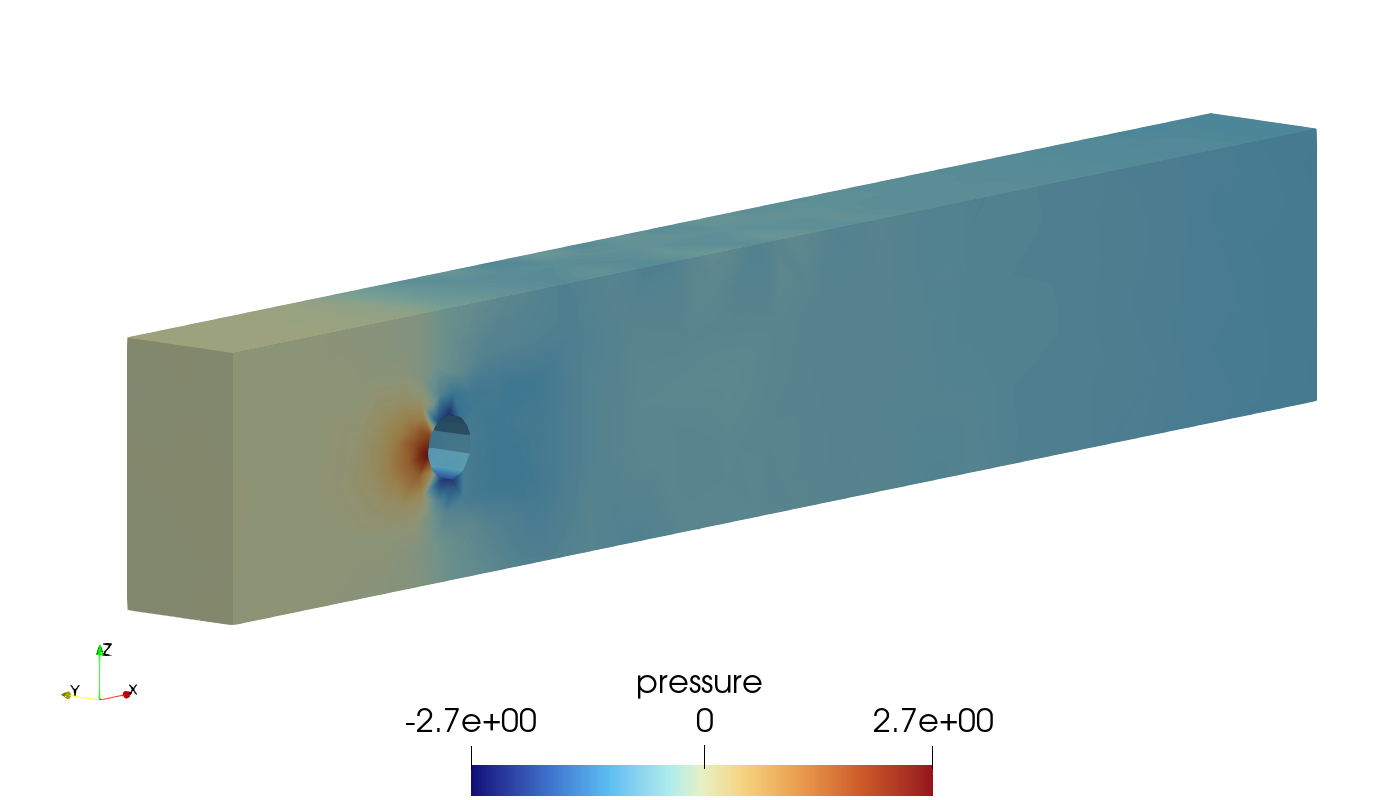
\includegraphics[width=\gridwidth]{pres_test2_coarse.png}}

    \subfloat[Cylinder Velocity (Coarse)]{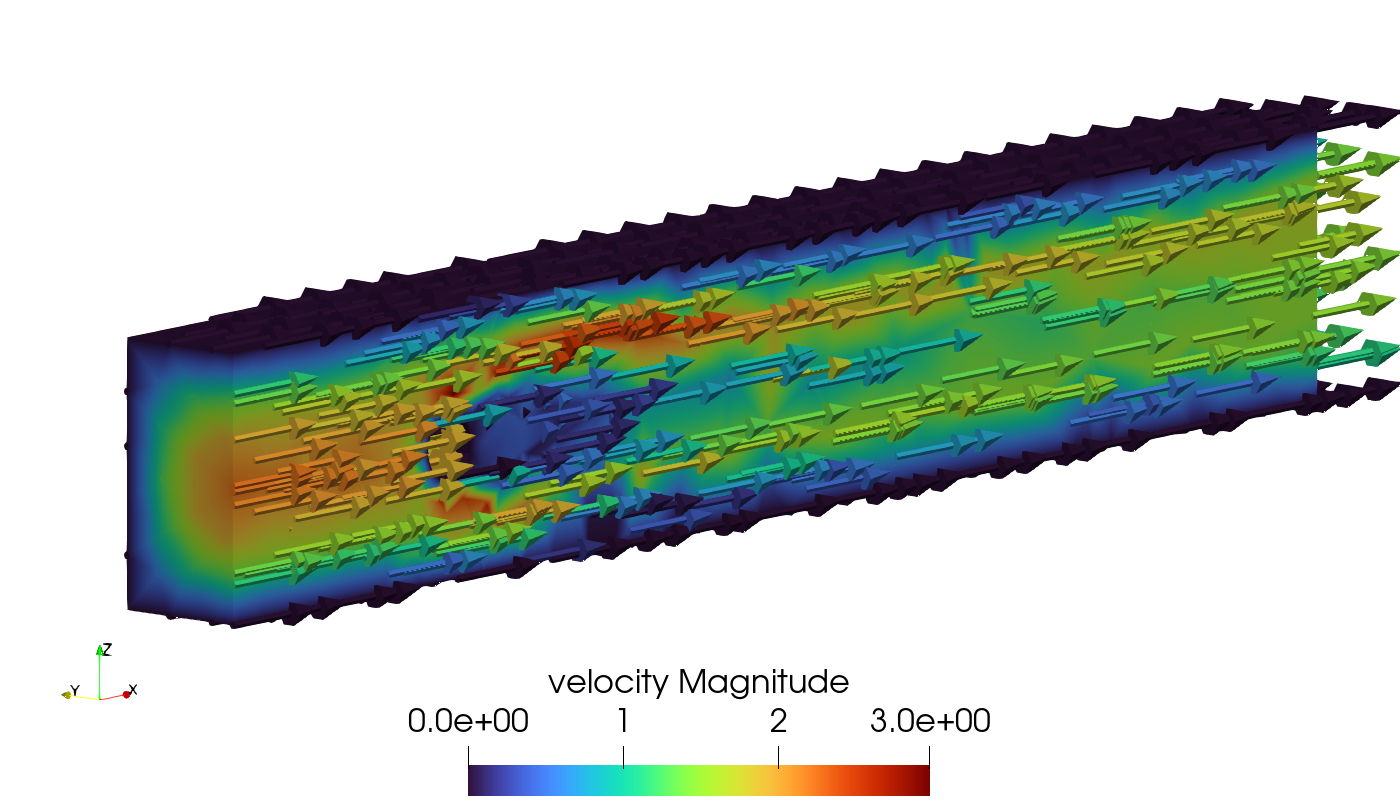
\includegraphics[width=\gridwidth]{glyph_cyl_test2.png}} 
    \hfill
    \subfloat[Cylinder Velocity (Coarse)]{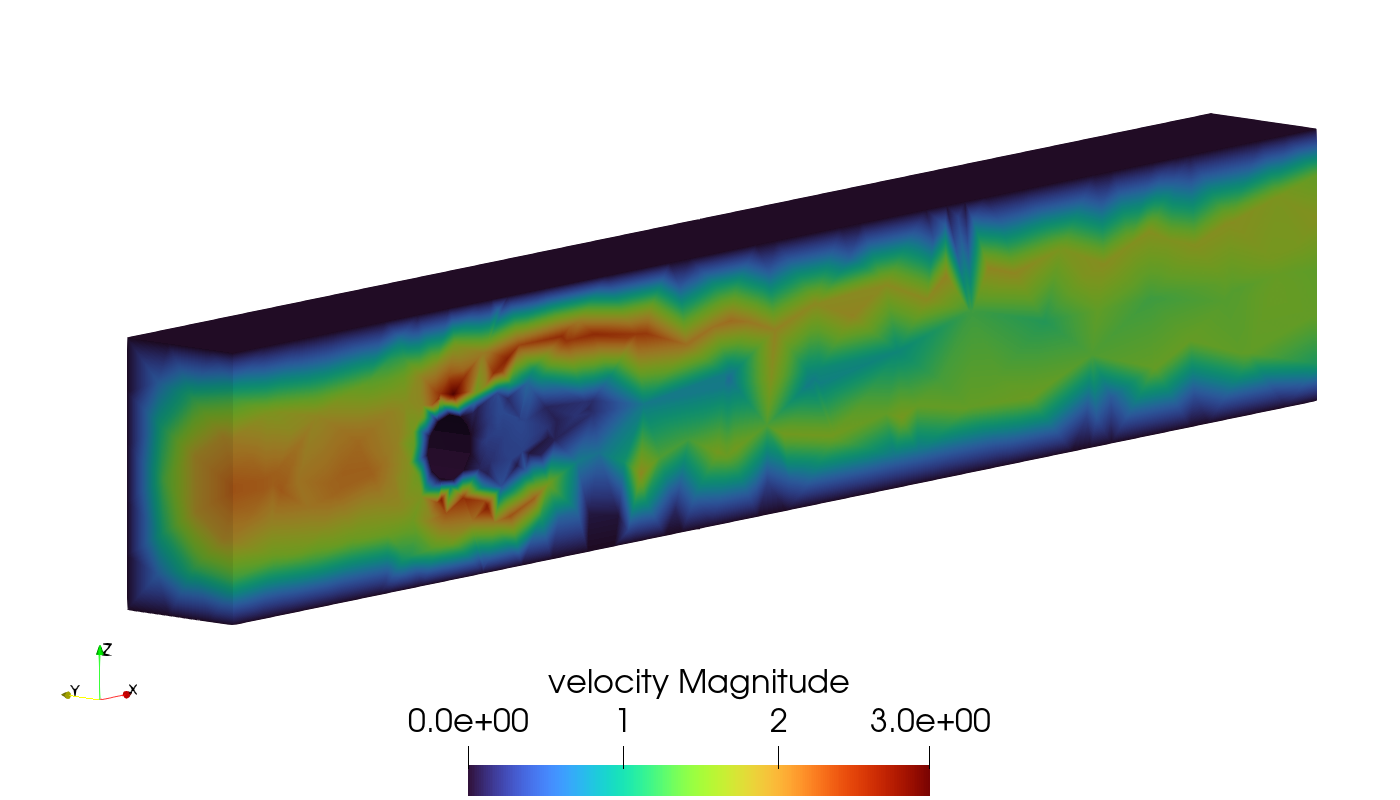
\includegraphics[width=\gridwidth]{vel_test2_coarse.png}}
    
    \caption{Selection of snapshots for the the 3D-2 steady test case.}
    \label{fig:3d_2_velocity__pressure_snapshots}
\end{figure}

%-------------------------------------------------------------
% 3D TEST CASE 3
%-------------------------------------------------------------

\begin{figure}[p]
    \centering
    % Define a local command to keep widths consistent and code readable
    \newcommand{\gridwidth}{0.48\textwidth}

    \subfloat[Cylinder Glyph (Fine)]{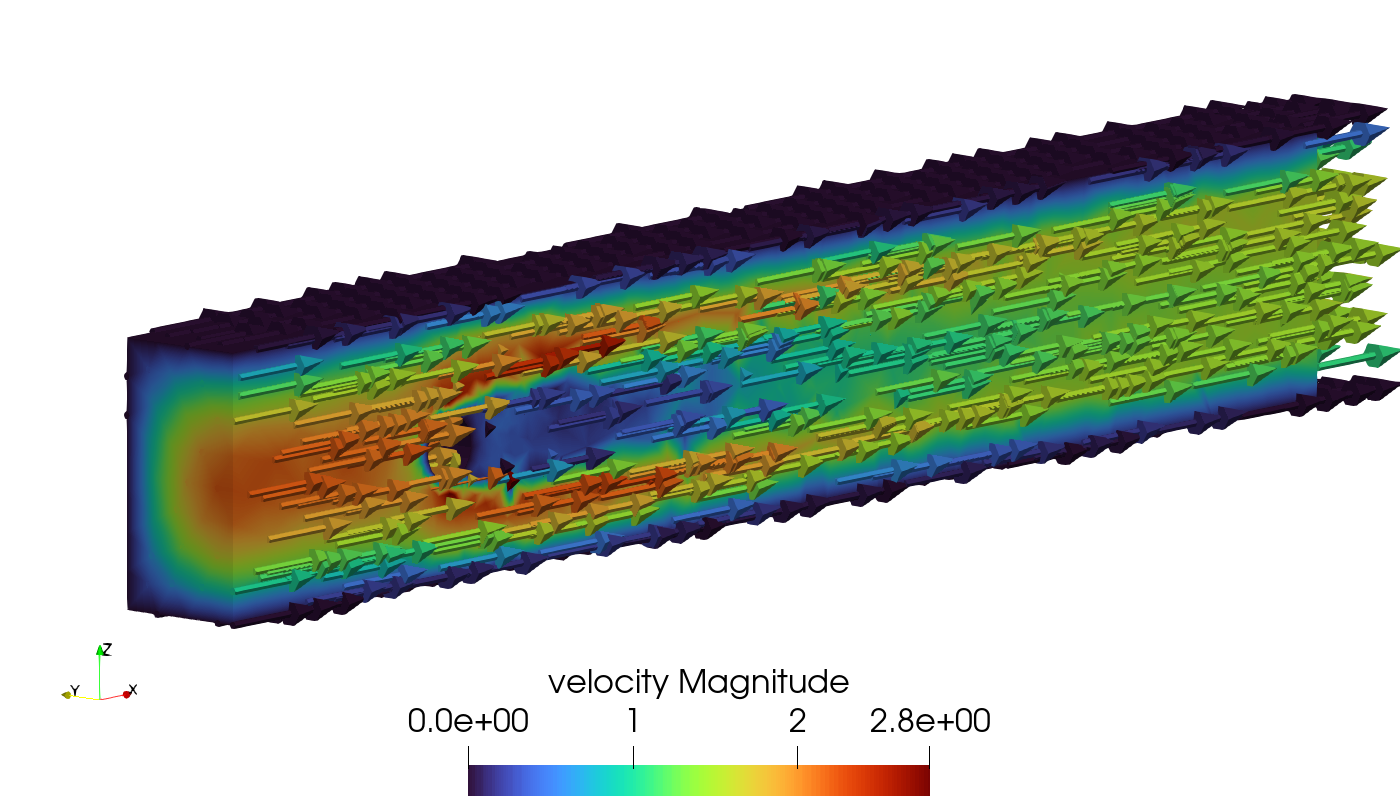
\includegraphics[width=\gridwidth]{vel_glyph_test3.png}}
    \hfill
    \subfloat[Cylinder Pressure (Fine)]{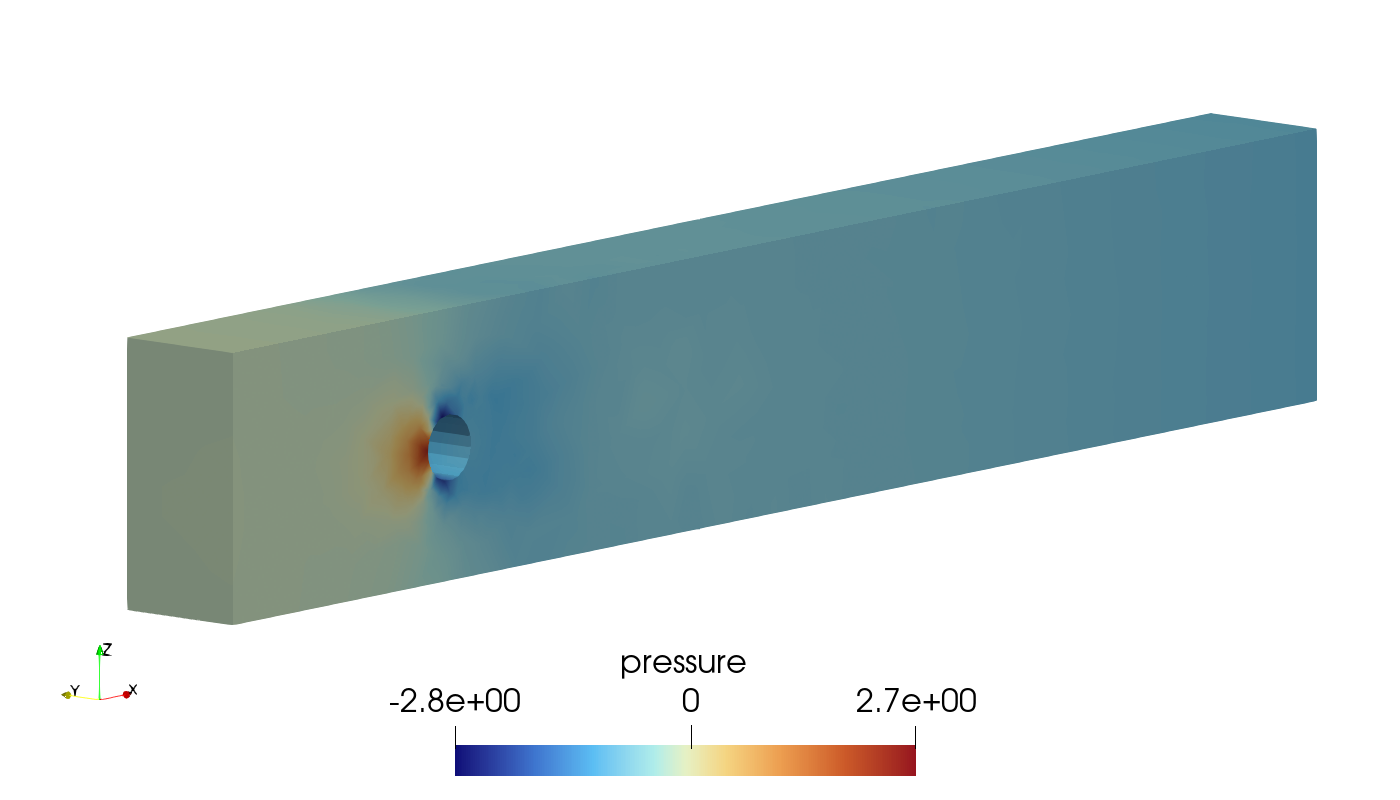
\includegraphics[width=\gridwidth]{pre_cyl_test3.png}} 

    \subfloat[Cylinder Stream Tracer (Coarse)]{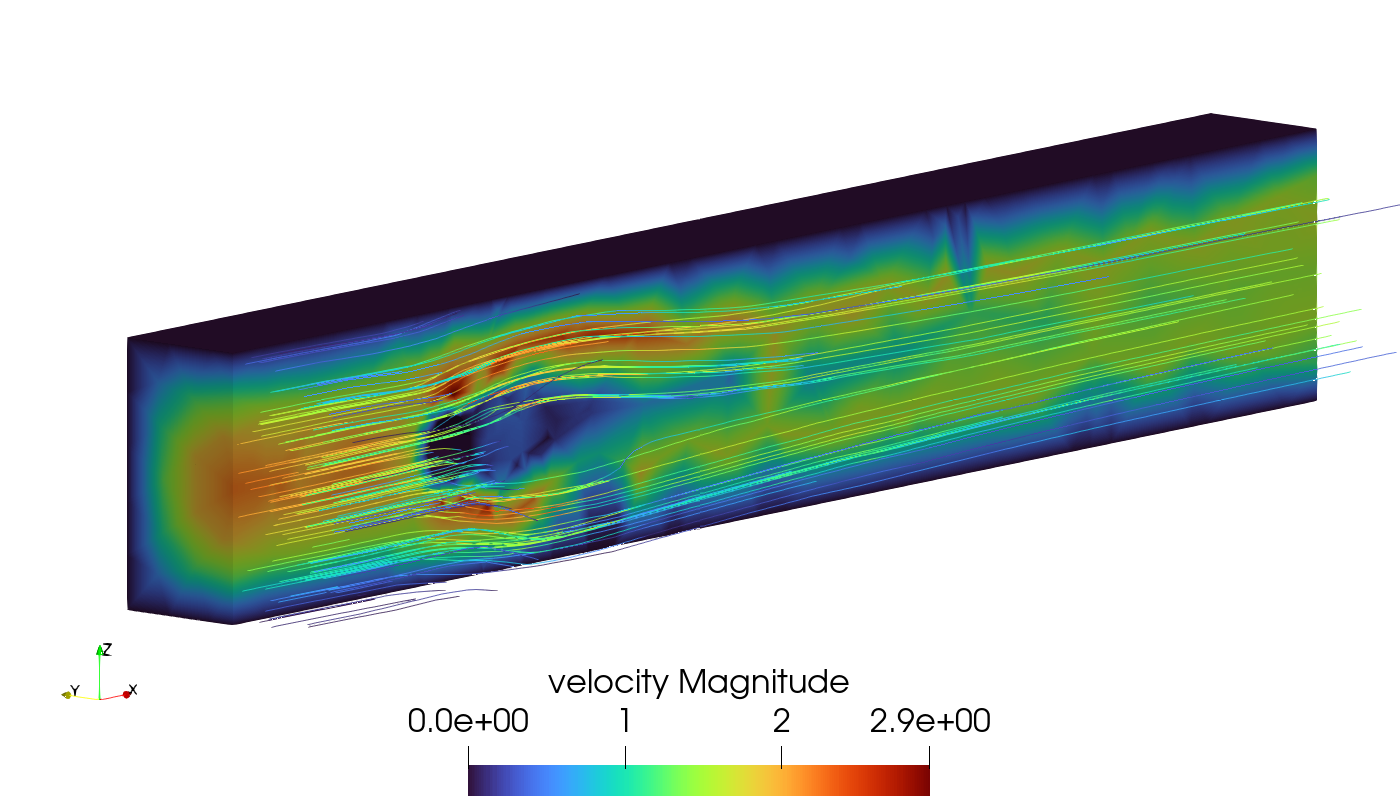
\includegraphics[width=\gridwidth]{cyl_st_coarse.png}}
    \hfill
    \subfloat[Cylinder Stream Tracer (Fine)]{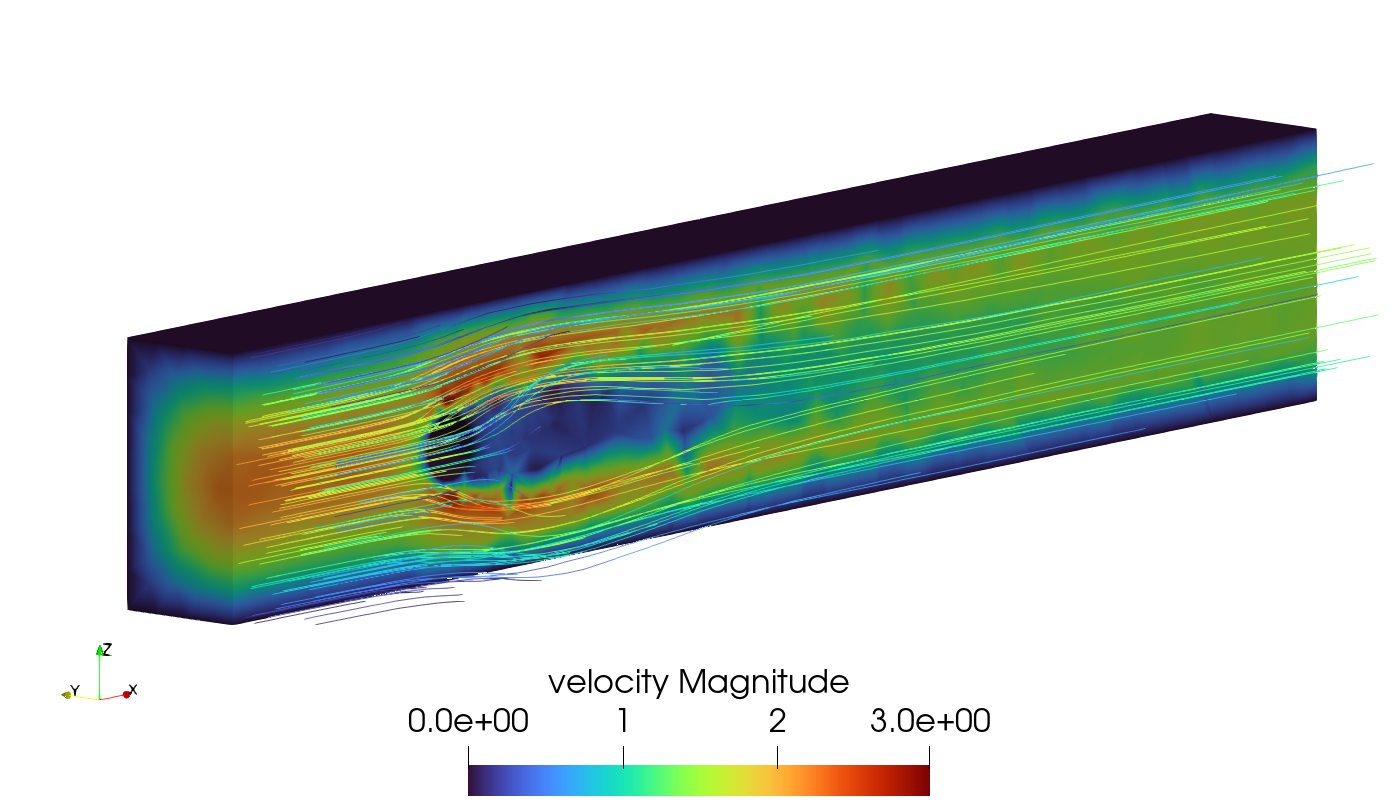
\includegraphics[width=\gridwidth]{vel_st_test3.png}}


    \hfill
    \subfloat[Parallelepiped Velocity (Fine)]{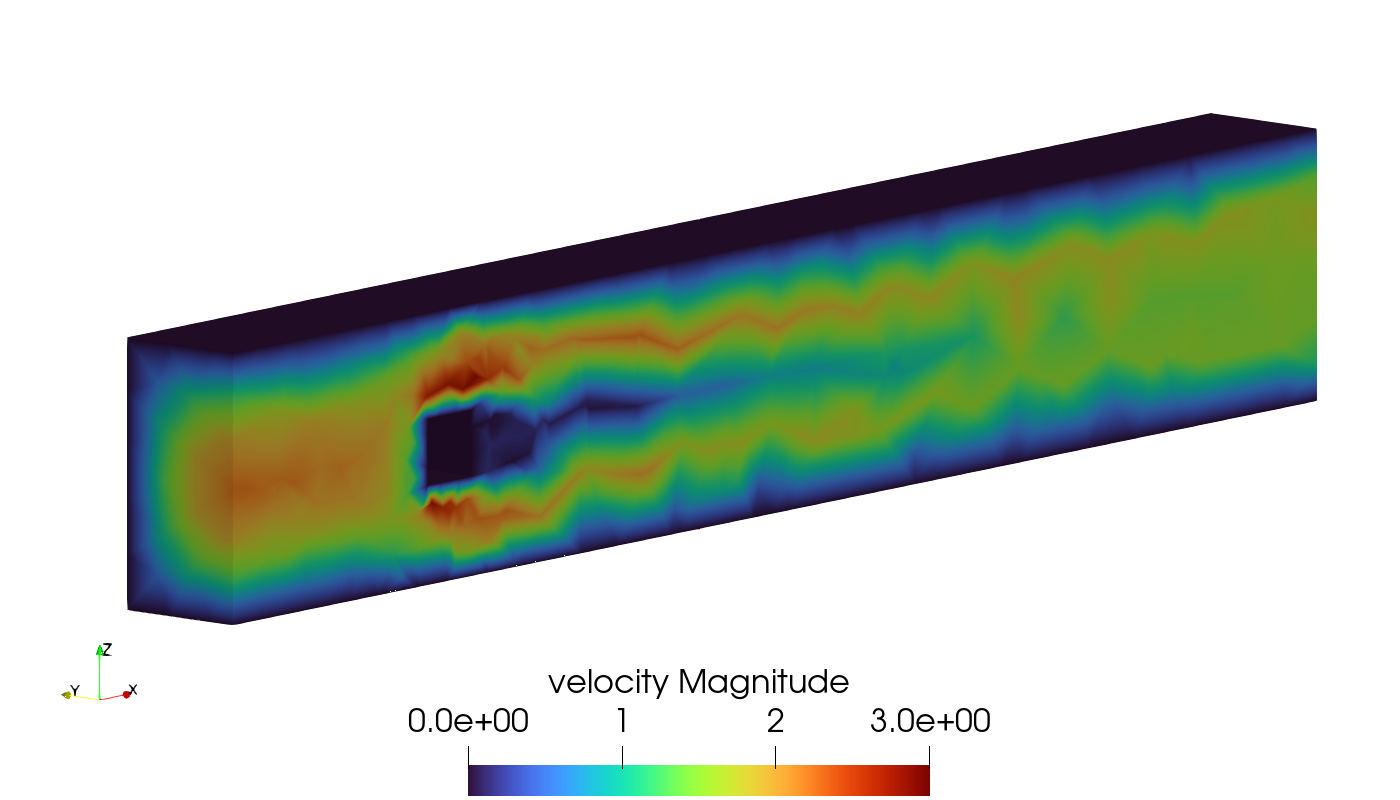
\includegraphics[width=\gridwidth]{par_test3_coarse.png}}
    \hfill
    \subfloat[Parallelepiped Pressure (Coarse)]{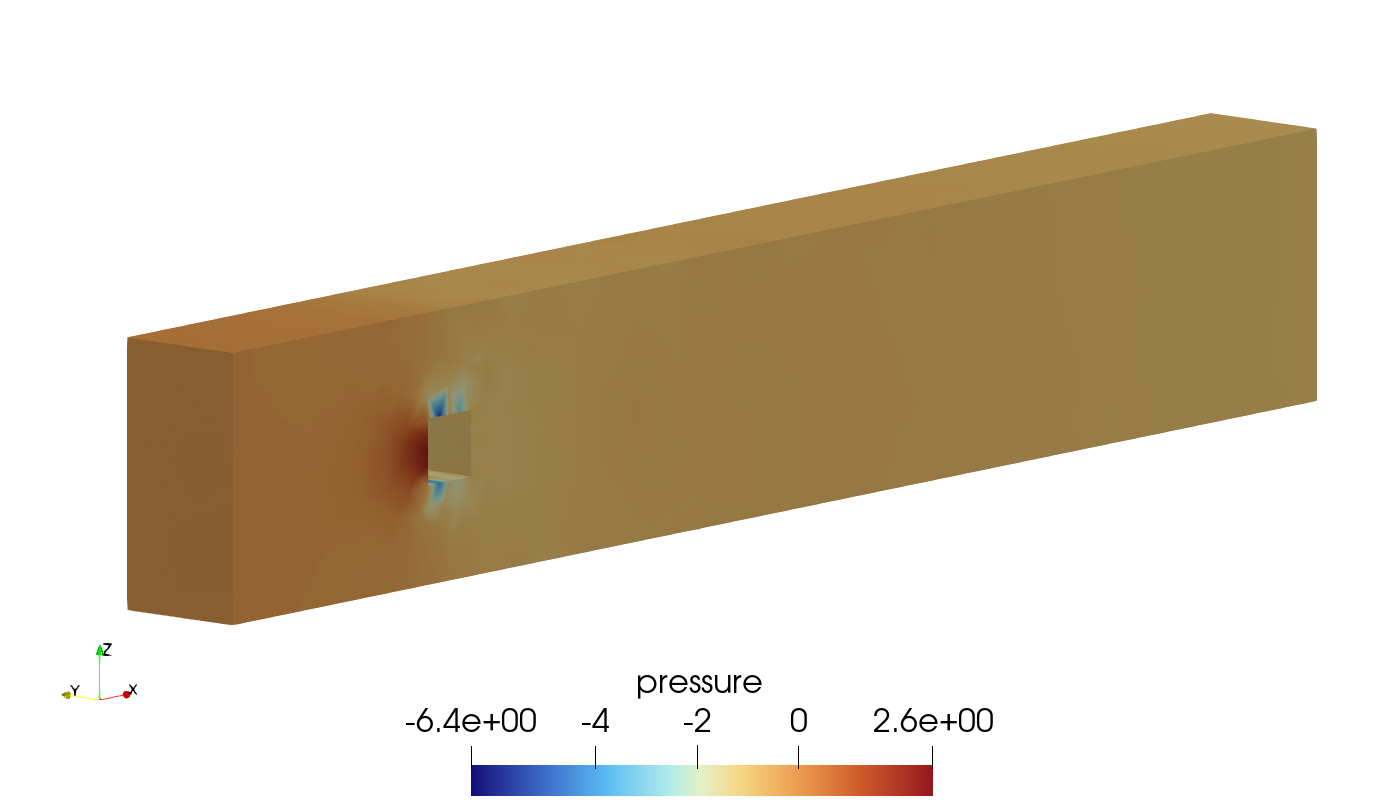
\includegraphics[width=\gridwidth]{par_test3_pressure.png}}

    \hfill
    \subfloat[Parallelepiped Stream Tracer (Fine)]{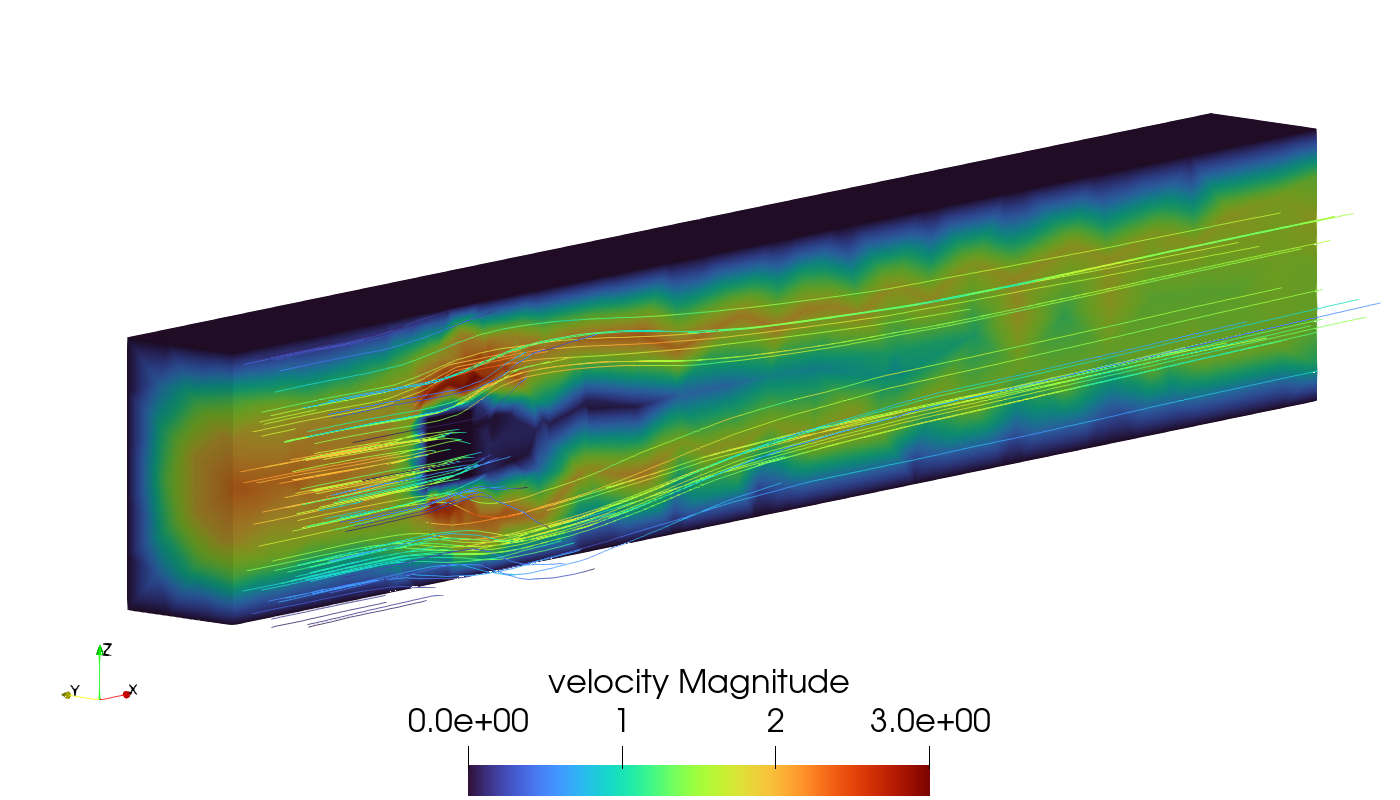
\includegraphics[width=\gridwidth]{par_test3_st.png}}
    \hfill
    \subfloat[Parallelepiped Pressure (Fine)]{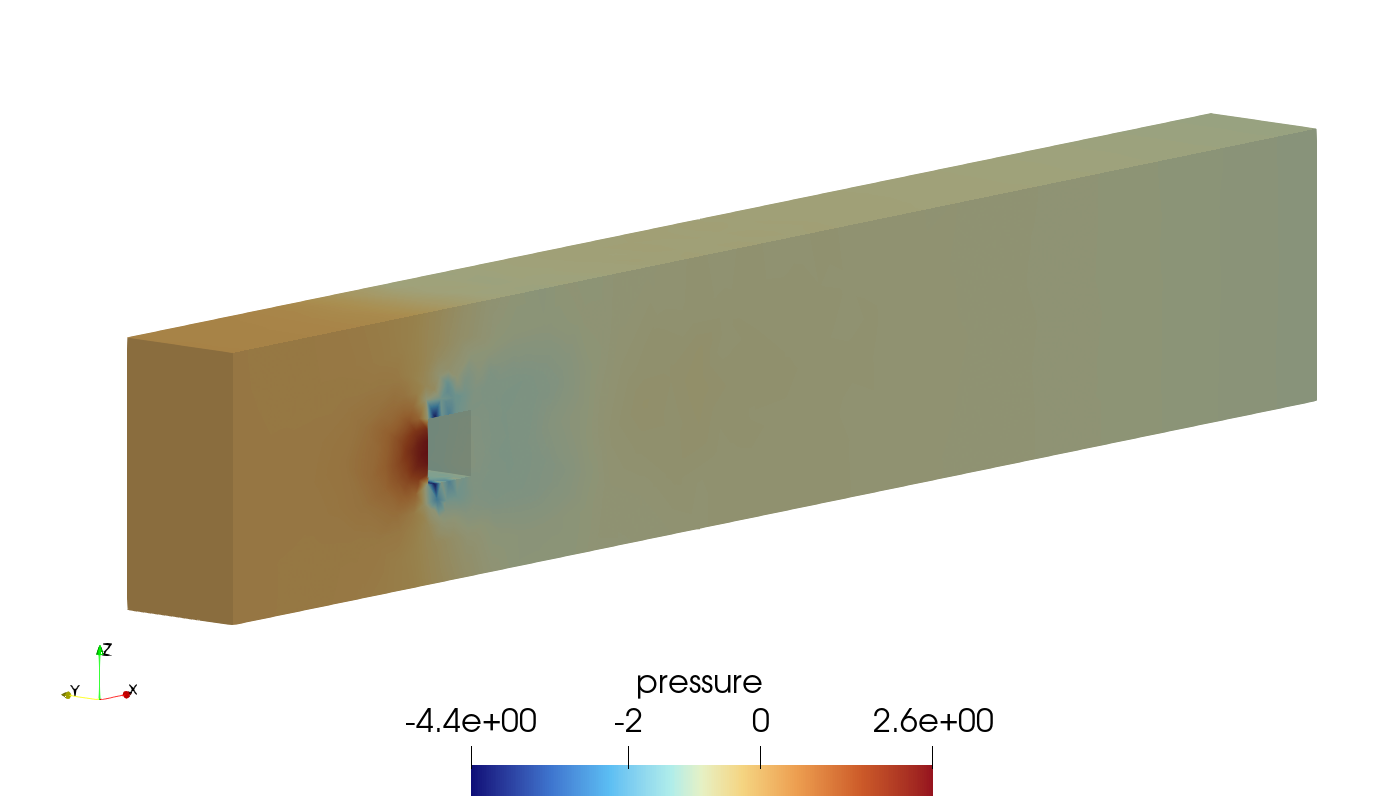
\includegraphics[width=\gridwidth]{pressure_fine.png}}
    
    \caption{Selection of snapshots for the the 3D-3 unsteady test case.}
    \label{fig:3d_3_velocity__pressure_snapshots}
\end{figure}

%-------------------------------------------------------------
% RE 1000 WITH CHORIN - TEMAM
%-------------------------------------------------------------
\begin{figure}[p]
    \centering
    % Define a local command to keep widths consistent and code readable
    \newcommand{\gridwidth}{0.48\textwidth}

    % Row 1: velocity
    \subfloat[Velocity \label{fig:ct_velocity}]{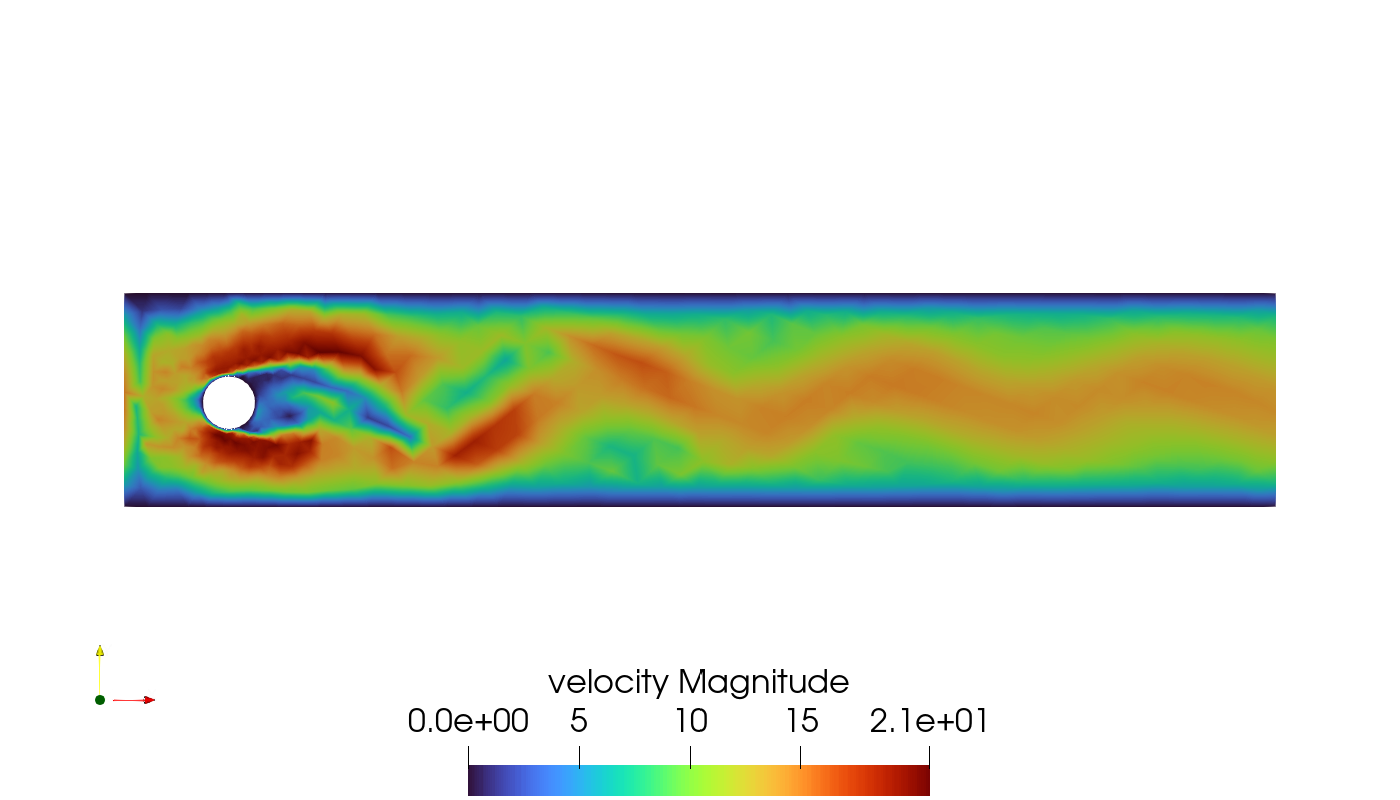
\includegraphics[width=\gridwidth]{Images/Test_cases/2D/Re_1000_CT/Screenshots/t_5_velocity.png}} 
    \hfill
    \subfloat[Pressure \label{fig:ct_pressure}]{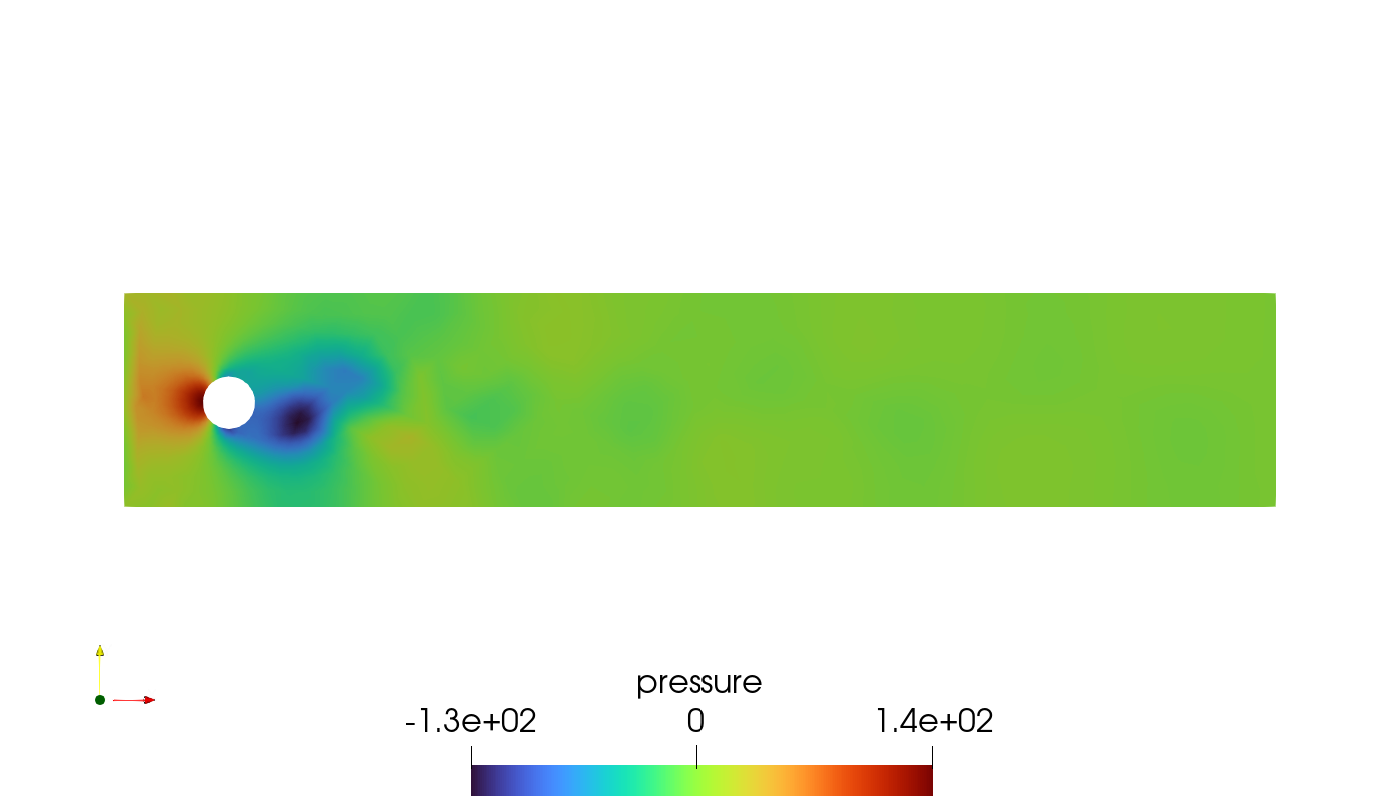
\includegraphics[width=\gridwidth]{Images/Test_cases/2D/Re_1000_CT/Screenshots/t_5_pressure.png}} \\

    \caption{Instantaneous velocity and pressure fields at $t = 5s$ on the fine mesh for $\Reynolds = 1000$ Chorin - Temam test case.}
    \label{fig:ct_velocity_pressure_snapshots}
\end{figure}


\cleardoublepage

%-------------------------------------------------------------------------
%	END OF YOUR DOCUMENT
%-------------------------------------------------------------------------
\end{document}